\documentclass{article}

% Packages
\usepackage[margin=1.5cm, includefoot, footskip=30pt]{geometry}
\usepackage{hyperref}
\usepackage{multicol}
\usepackage{booktabs}
\usepackage{xstring}
\usepackage{subcaption}
\usepackage{graphicx}
\usepackage{amsmath}
\usepackage{standalone}
\usepackage{fancyvrb}

\usepackage{tikz}
\usetikzlibrary{calc, shapes, patterns}

\usepackage[backend=biber, firstinits=false, backref=false, url=true,
            isbn=true, style=numeric]{biblatex}
\addbibresource{bibliography.bib}

% Title
\title{A numerical study of fixation probabilities for strategies in the
       Iterated Prisoner's Dilemma}
\author{Marc Harper \and Vincent Knight} % TODO Authors?
\date{}


\begin{document}

\maketitle

\begin{abstract}
    The Iterated Prisoner's Dilemma is a well established framework for
    the study of emergent behaviour. In this paper an extensive numerical
    study of the evolutionary dynamics of this framework are presented.

    Fixation probabilities for Moran processes are obtained for 172
    different strategies. This is done in both a standard 200 turn
    interaction and a noisy setting.

    To the authors knowledge this is the largest
    such study. It allows for insights about the behaviour and
    performance of strategies with regard to their survival in an
    evolutionary setting.
\end{abstract}  % TODO Add main conclusion/finding.

\section{Introduction}\label{sec:introduction}

Since the formulation of the Moran Process in \cite{Moran1957}, this model of
evolutionary population dynamics has been used to gain insights about the
evolutionary stability of strategies in a number of settings. Similarly since
the first Iterated Prisoner's Dilemma (IPD) tournament described in
\cite{Axelrod1980a} the Prisoner's dilemma has been used to understand the
evolution of cooperative behaviour in complex systems.

The analytical models of a Moran process are based on the relative fitness
between two strategies and take this to be a fixed value \(r\) \cite{Nowak}.
This is a valid model for simple strategies of the Prisoner's Dilemma such as to
\textit{always cooperate} or \textit{always defect}. This manuscript provides a
detailed numerical analysis of \textbf{172} complex and adaptive strategies for
the IPD\@. In this case the relative fitness of a strategy is dependent on the
population distribution.

Further deviations from the analytical model occur when interactions between
players are subject to uncertainty. This is referred to as noise and has been
considered in the IPD setting in \cite{Bendor1993, Nowak1993, Wu1995}. Noise is
also considered here.

This work provides answers to the following questions:

\begin{enumerate}
    \item What strategies are good invaders?
    \item What strategies are good at resisting invasion?
    \item How does the population size affect these findings?
\end{enumerate}

Figure~\ref{fig:moran_process} shows a diagrammatic representation of the Moran
process. The Moran process is a stochastic birth death process on a finite
population in which the population size stays constant over time. Individuals
are \textbf{selected} according to a given fitness landscape. Once selected, a
given individual is reproduced and similarly another individual is chosen to be
removed from the population. In some settings mutation is also considered but
without mutation (the case considered in this work) this process will arrive at
an absorbing state where the population is entirely made up of a single
individual. The probability with which a given strategy is the survivor is
called the absorption probability. A more detailed analytic description of this
is given in Section~\ref{sec:validation}.

\begin{figure}[!hbtp]
    \centering
    \documentclass{standalone}
\usepackage{tikz}
\usetikzlibrary{calc, shapes, patterns}

\begin{document}
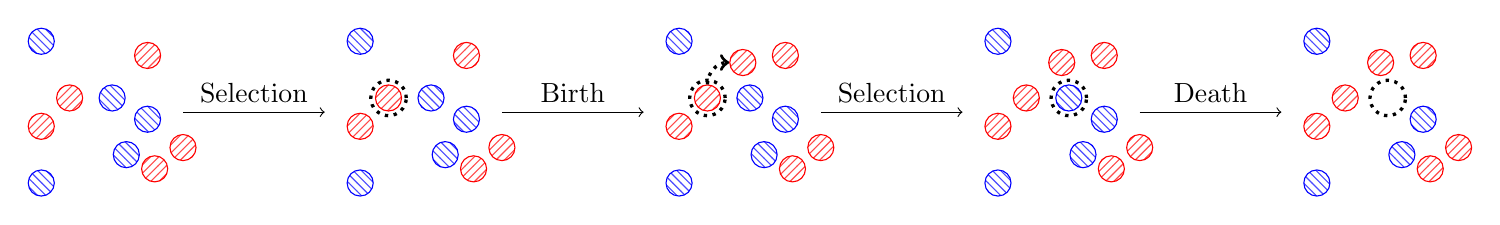
\begin{tikzpicture}[scale=.9]
	\node (A1) at (-1, -1) [circle, pattern=north west lines, pattern
        color=blue!70, draw=blue] {};
	\node (A2) at (-1, 1) [circle, pattern=north west lines, pattern
        color=blue!70, draw=blue] {};
	\node (A3) at (0, .2) [circle, pattern=north west lines, pattern
        color=blue!70, draw=blue] {};
	\node (A4) at (.2, -.6) [circle, pattern=north west lines, pattern
        color=blue!70, draw=blue] {};
	\node (A5) at (.5, -0.1) [circle, pattern=north west lines, pattern
        color=blue!70, draw=blue] {};
	\node (B1) at (-1, -.2) [circle, pattern=north east lines, pattern
        color=red!70, draw=red] {};
	\node (B2) at (1, -.5) [circle, pattern=north east lines, pattern
        color=red!70, draw=red] {};
	\node (B3) at (.5, .8) [circle, pattern=north east lines, pattern
        color=red!70, draw=red] {};
	\node (B4) at (-.6, .2) [circle, pattern=north east lines, pattern
        color=red!70, draw=red] {};
	\node (B5) at (.6, -.8) [circle, pattern=north east lines, pattern
        color=red!70, draw=red] {};

	\draw [->] (1, 0) -- (3, 0) node [above, pos=0.5] {Selection};

	\node (A1) at ($(A1) + (4.5, 0)$) [circle, pattern=north west lines,
        pattern color=blue!70, draw=blue] {};
	\node (A2) at ($(A2) + (4.5, 0)$) [circle, pattern=north west lines,
        pattern color=blue!70, draw=blue] {};
	\node (A3) at ($(A3) + (4.5, 0)$) [circle, pattern=north west lines,
        pattern color=blue!70, draw=blue] {};
	\node (A4) at ($(A4) + (4.5, 0)$) [circle, pattern=north west lines,
        pattern color=blue!70, draw=blue] {};
    \node (A5) at ($(A5) + (4.5, 0)$) [circle, pattern=north west lines,
        pattern color=blue!70, draw=blue] {};
	\node (B1) at ($(B1) + (4.5, 0)$) [circle, pattern=north east lines,
        pattern color=red!70, draw=red] {};
	\node (B2) at ($(B2) + (4.5, 0)$) [circle, pattern=north east lines,
        pattern color=red!70, draw=red] {};
	\node (B3) at ($(B3) + (4.5, 0)$) [circle, pattern=north east lines,
        pattern color=red!70, draw=red] {};
	\node (B4) at ($(B4) + (4.5, 0)$) [circle, pattern=north east lines,
        pattern color=red!70, draw=red] {};
	\node (B5) at ($(B5) + (4.5, 0)$) [circle, pattern=north east lines,
        pattern color=red!70, draw=red] {};

	\draw [dotted, very thick] (B4) circle (.25cm);

	\draw [->] (5.5, 0) -- (7.5, 0) node [above, pos=0.5] {Birth};

	\node (A1) at ($(A1) + (4.5, 0)$) [circle, pattern=north west lines,
        pattern color=blue!70, draw=blue] {};
	\node (A2) at ($(A2) + (4.5, 0)$) [circle, pattern=north west lines,
        pattern color=blue!70, draw=blue] {};
	\node (A3) at ($(A3) + (4.5, 0)$) [circle, pattern=north west lines,
        pattern color=blue!70, draw=blue] {};
	\node (A4) at ($(A4) + (4.5, 0)$) [circle, pattern=north west lines,
        pattern color=blue!70, draw=blue] {};
    \node (A5) at ($(A5) + (4.5, 0)$) [circle, pattern=north west lines,
        pattern color=blue!70, draw=blue] {};
	\node (B1) at ($(B1) + (4.5, 0)$) [circle, pattern=north east lines,
        pattern color=red!70, draw=red] {};
	\node (B2) at ($(B2) + (4.5, 0)$) [circle, pattern=north east lines,
        pattern color=red!70, draw=red] {};
	\node (B3) at ($(B3) + (4.5, 0)$) [circle, pattern=north east lines,
        pattern color=red!70, draw=red] {};
	\node (B4) at ($(B4) + (4.5, 0)$) [circle, pattern=north east lines,
        pattern color=red!70, draw=red] {};
	\node (B5) at ($(B5) + (4.5, 0)$) [circle, pattern=north east lines,
        pattern color=red!70, draw=red] {};

	\draw [dotted, very thick] (B4) circle (.25cm);
	\node (B6) at ($(B4) + (0.5, 0.5)$) [circle, pattern=north east lines,
        pattern color=red!70, draw=red] {};
	\draw [->, dotted, very thick] (B4) [out=90, in=180] to (B6);

	\draw [->] (10, 0) -- (12, 0) node [above, pos=0.5] {Selection};

	\node (A1) at ($(A1) + (4.5, 0)$) [circle, pattern=north west lines,
        pattern color=blue!70, draw=blue] {};
	\node (A2) at ($(A2) + (4.5, 0)$) [circle, pattern=north west lines,
        pattern color=blue!70, draw=blue] {};
	\node (A3) at ($(A3) + (4.5, 0)$) [circle, pattern=north west lines,
        pattern color=blue!70, draw=blue] {};
	\node (A4) at ($(A4) + (4.5, 0)$) [circle, pattern=north west lines,
        pattern color=blue!70, draw=blue] {};
    \node (A5) at ($(A5) + (4.5, 0)$) [circle, pattern=north west lines,
        pattern color=blue!70, draw=blue] {};
	\node (B1) at ($(B1) + (4.5, 0)$) [circle, pattern=north east lines,
        pattern color=red!70, draw=red] {};
	\node (B2) at ($(B2) + (4.5, 0)$) [circle, pattern=north east lines,
        pattern color=red!70, draw=red] {};
	\node (B3) at ($(B3) + (4.5, 0)$) [circle, pattern=north east lines,
        pattern color=red!70, draw=red] {};
	\node (B4) at ($(B4) + (4.5, 0)$) [circle, pattern=north east lines,
        pattern color=red!70, draw=red] {};
	\node (B5) at ($(B5) + (4.5, 0)$) [circle, pattern=north east lines,
        pattern color=red!70, draw=red] {};
	\node (B6) at ($(B6) + (4.5, 0)$) [circle, pattern=north east lines,
        pattern color=red!70, draw=red] {};

	\draw [dotted, very thick] (A3) circle (.25cm);

	\draw [->] (14.5, 0) -- (16.5, 0) node [above, pos=0.5] {Death};

	\node (A1) at ($(A1) + (4.5, 0)$) [circle, pattern=north west lines,
        pattern color=blue!70, draw=blue] {};
	\node (A2) at ($(A2) + (4.5, 0)$) [circle, pattern=north west lines,
        pattern color=blue!70, draw=blue] {};
	\node (A3) at ($(A3) + (4.5, 0)$) {};
	\node (A4) at ($(A4) + (4.5, 0)$) [circle, pattern=north west lines,
        pattern color=blue!70, draw=blue] {};
    \node (A5) at ($(A5) + (4.5, 0)$) [circle, pattern=north west lines,
        pattern color=blue!70, draw=blue] {};
	\node (B1) at ($(B1) + (4.5, 0)$) [circle, pattern=north east lines,
        pattern color=red!70, draw=red] {};
	\node (B2) at ($(B2) + (4.5, 0)$) [circle, pattern=north east lines,
        pattern color=red!70, draw=red] {};
	\node (B3) at ($(B3) + (4.5, 0)$) [circle, pattern=north east lines,
        pattern color=red!70, draw=red] {};
	\node (B4) at ($(B4) + (4.5, 0)$) [circle, pattern=north east lines,
        pattern color=red!70, draw=red] {};
	\node (B5) at ($(B5) + (4.5, 0)$) [circle, pattern=north east lines,
        pattern color=red!70, draw=red] {};
	\node (B6) at ($(B6) + (4.5, 0)$) [circle, pattern=north east lines,
        pattern color=red!70, draw=red] {};

	\draw [dotted, very thick] (A3) circle (.25cm);
\end{tikzpicture}
\end{document}

    \caption{A diagrammatic representation of a Moran process}
    \label{fig:moran_process}
\end{figure}

The Moran process was initially introduced in \cite{Moran1957} in a genetic
setting. It has sine been used in a variety of settings including the
understanding of the spread of cooperative behaviour. However, as stated before,
these mainly consider non sophisticated strategies. Some work has looked at
evolutionary stability of strategies within the Prisoner's Dilemma \cite{Li2014}
but this is not done in the more widely used setting of the Moran process but in
terms of infinite population stability. In \cite{Baek2016} Moran processes are
looked at in a theoretic framework for a small subset of strategies. In
\cite{Lee2015} machine learning techniques are used to train a strategy capable
of resisting invasion and also invade any memory one strategy. Recent work
\cite{Hilbe2017} has investigated the effect of memory length on strategy
performance and the emergence of cooperation but this is not done in Moran
process context and only considers specific cases of memory 2 strategies.
% TODO Is this OK? We should add more.

The contribution of this work is a detailed and extensive analysis of absorption
probabilities for 172 strategies. These strategies and the numerical simulations
are from~\cite{axelrodproject} which is an open source research library written
for the study of the IPD\@. The strategies and simulation frameworks are
automatically tested in accordance to best practice. The large number of
strategies are available thanks to the open source nature of the project with
over 40 contributions made by different programmers. Thus by considering Moran
processes with population size greater than 2 we are taking in to account the
effect of complex population dynamics. By considering sophisticated strategies
we are taking in to effect the reputation of a strategy during each interaction.

Section~\ref{sec:methodology} will explain the methodological approach used,
Section~\ref{sec:validation} will validate the methodology by comparing
simulated results to analytical results. The main results of this manuscript are
presented in Section~\ref{sec:numerical_results} which will present a detailed
analysis of all the data generated. Finally, Section~\ref{sec:conclusion} will
conclude and offer future avenues for the work presented here.

\section{Methodology}\label{sec:methodology}

To carry out this large numerical experiment 172 strategies are used from
\cite{axelrodproject}. These include 169 default strategies in the library at
the time (excluding strategies classified as having a long run time) as well as
the following 3 finite state machine machine strategies \cite{Ashlock2006}:

% TODO Include details about the 3 extra FSM strategies.
% Possibly draw pictorial representations?

Appendix~\ref{app:list_of_players} shows all the players in question. More
information about each player can be obtained in the documentation for
\cite{axelrodproject}. The memory depth of the used strategies is shown in
Table~\ref{tbl:memory_depth_count}.

\begin{table}[!hbtp]
    \centering
        \begin{subfigure}[t]{\textwidth}
            \centering
                \begin{tabular}{lrrrrrrrrrrrrrrrr}
\toprule
Memory Depth &   0   &   1   &   2   &   3   &   4   &   5   &   6   &   9   &   10  &   11  &   12  &   16  &   20  &   40  &   200 &  \(\infty\)   \\
\midrule
Count &     3 &    31 &    12 &     8 &     2 &     6 &     1 &     1 &     5 &     1 &     1 &     2 &     2 &     2 &     1 &    86 \\
\bottomrule
\end{tabular}

                \caption{Memory depth}
                \label{tbl:memory_depth_count}
        \end{subfigure}
        \vspace{.5cm}

        \begin{subfigure}[t]{\textwidth}
            \centering
                \begin{tabular}{lr}
\toprule
Stochastic &  Count \\
\midrule
     False &    123 \\
      True &     49 \\
\bottomrule
\end{tabular}

                \caption{Stochastic versus deterministic}
                \label{tbl:stochastic_count}
        \end{subfigure}
        \caption{Summary of properties of used strategies}
\end{table}

All strategies are paired and these pairs are used in 2000 repetitions of a
Moran process assuming a starting population of \((N/2, N/2)\). This is repeated
for even \(N\) between 2 and 14. The fixation probability is then estimated for
each value of \(N\).

Note that due to the high computational cost of these experiments, for any given
interaction between two players within the Moran process the outcome is sampled
from a pre computed cache of 1000 match outcomes. This is carried out using the
approximate Moran process implemented in \cite{axelrodproject}.

As an example, Figure~\ref{fig:players_with_most_scores} shows the scores
between two players that over the 1000 outcomes gives 971 different scores.

\begin{figure}[!htbp]
    \centering
    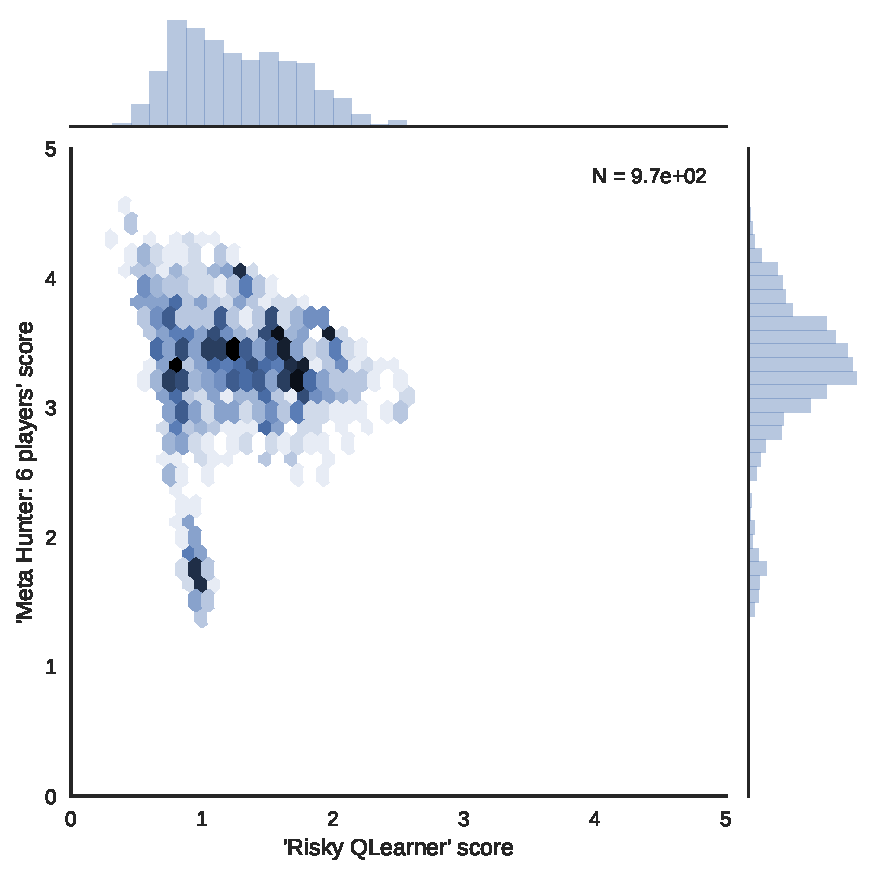
\includegraphics[width=.4\textwidth]{../img/players_with_most_scores.pdf}
    \caption{All possible scores for the pair of strategies that have the most
    different number of match outcomes}
    \label{fig:players_with_most_scores}
\end{figure}

A variety of software libraries have been used in this work:

\begin{itemize}
    \item The Axelrod library (IPD strategies and Moran processes)
        \cite{axelrodproject}.
    \item The matplotlib library (visualisation) \cite{hunter2007matplotlib}.
    \item The pandas and numpy libraries (data manipulation)
        \cite{mckinney2010data, walt2011numpy}.
\end{itemize}

Section~\ref{sec:validation} will validate this approach against theoretic
results.

\section{Validation}\label{sec:validation}

As described in \cite{Nowak} Consider the payoff matrix:

\begin{equation}\label{equ:payoff_matrix}
    M = \begin{pmatrix}
        a, b\\
        c, d
        \end{pmatrix}
\end{equation}

The expected payoffs of \(i\) players of the first type in a population with \(N
- i\) players of the second type are given by:

\begin{equation}\label{equ:expected_payoff_one}
    F_i = \frac{a(i - 1) + b(N - i)}{N - 1}
\end{equation}

\begin{equation}\label{equ:expected_payoff_two}
    G_i = \frac{ci + d(N - i - 1)}{N - 1}
\end{equation}

With an intensity of selection \(\omega\) the fitness of both strategies is
given by:

\begin{equation}\label{equ:expected_payoff_one}
    f_i = 1 - \omega + \omega F_i
\end{equation}

\begin{equation}\label{equ:expected_payoff_two}
    g_i = 1 - \omega + \omega G_i
\end{equation}

The transitions within the birth death process that underpins the Moran process
are then given by:

\begin{align}
	p_{i, i+1}&= \frac{if_i}{if_i+(N-i)g_i}\frac{N-i}{N}\label{equ:p_up}\\
	p_{i, i-1}&= \frac{(N-i)g_i}{if_i+(N-i)g_i}\frac{i}{N}\label{equ:p_down}\\
	p_{ii} &= 1 - p_{i, i+1} - p_{i, i-1}\label{equ:p_stay}
\end{align}

Using this it is a known result that the fixation probability of the first
strategy in a population of \(i\) individuals of the first type (and \(N-i\)
individuals of the second. We have:

\begin{equation}\label{equ:fixation_probability}
x_i = \frac{1 + \sum_{j=1}^{i-1}\prod_{k=1}^{j}\gamma_j}{1 + \sum_{j=1}^{N-1}
      \prod_{k=1}^{j}\gamma_j}
\end{equation}

where:

\[
\gamma_j = \frac{p_{j, j-1}}{p_{j, j+1}}
\]

Using this comparisons of \(x_{N/2}\) are shown in
Figure~\ref{fig:comparison_deterministic}. Note that these are all deterministic
strategies and show a perfect match up between the expected value of
(\ref{equ:fixation_probability}) and the actual Moran process for all
strategies pairs.

\begin{figure}[!hbtp]
    \centering
    \begin{subfigure}[t]{.3\textwidth}
        \centering
        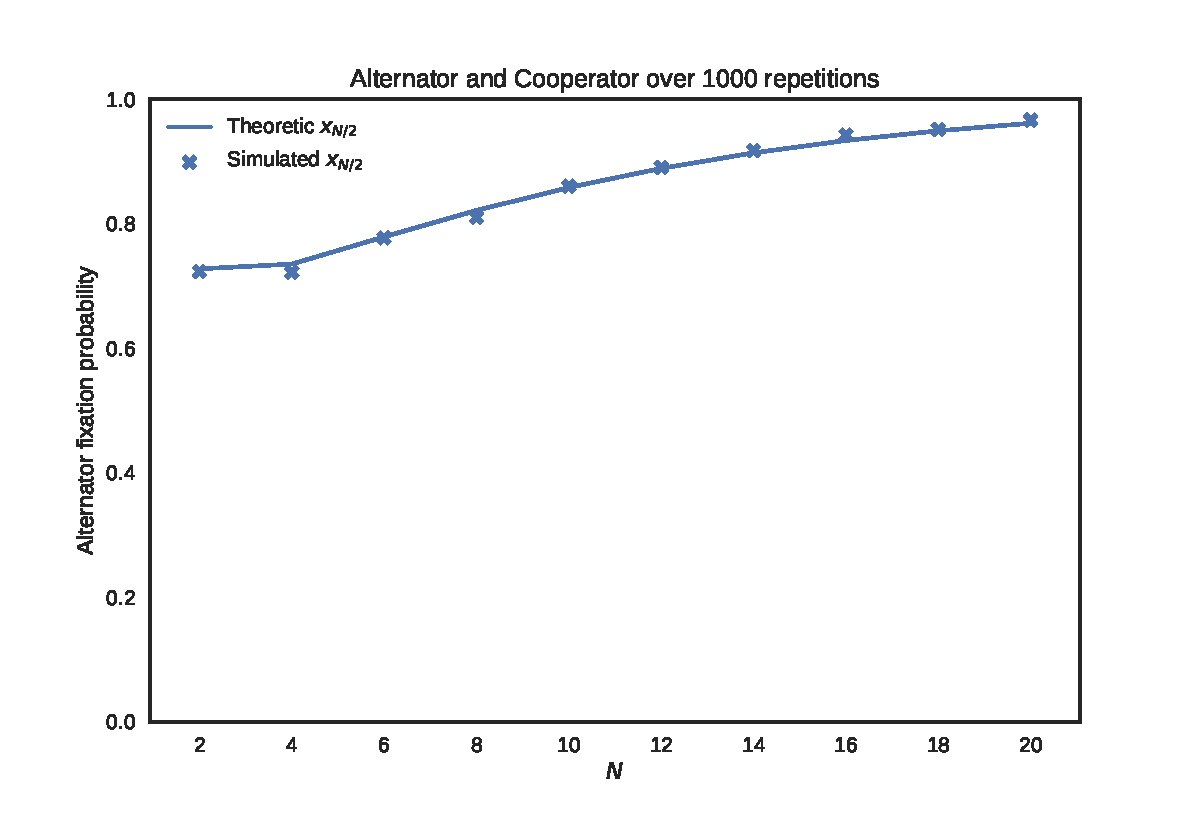
\includegraphics[width=.8\textwidth]{../img/Alternator_v_Cooperator.pdf}
        \caption{Alternator and Cooperator}
    \end{subfigure}%
    ~
    \begin{subfigure}[t]{.3\textwidth}
        \centering
        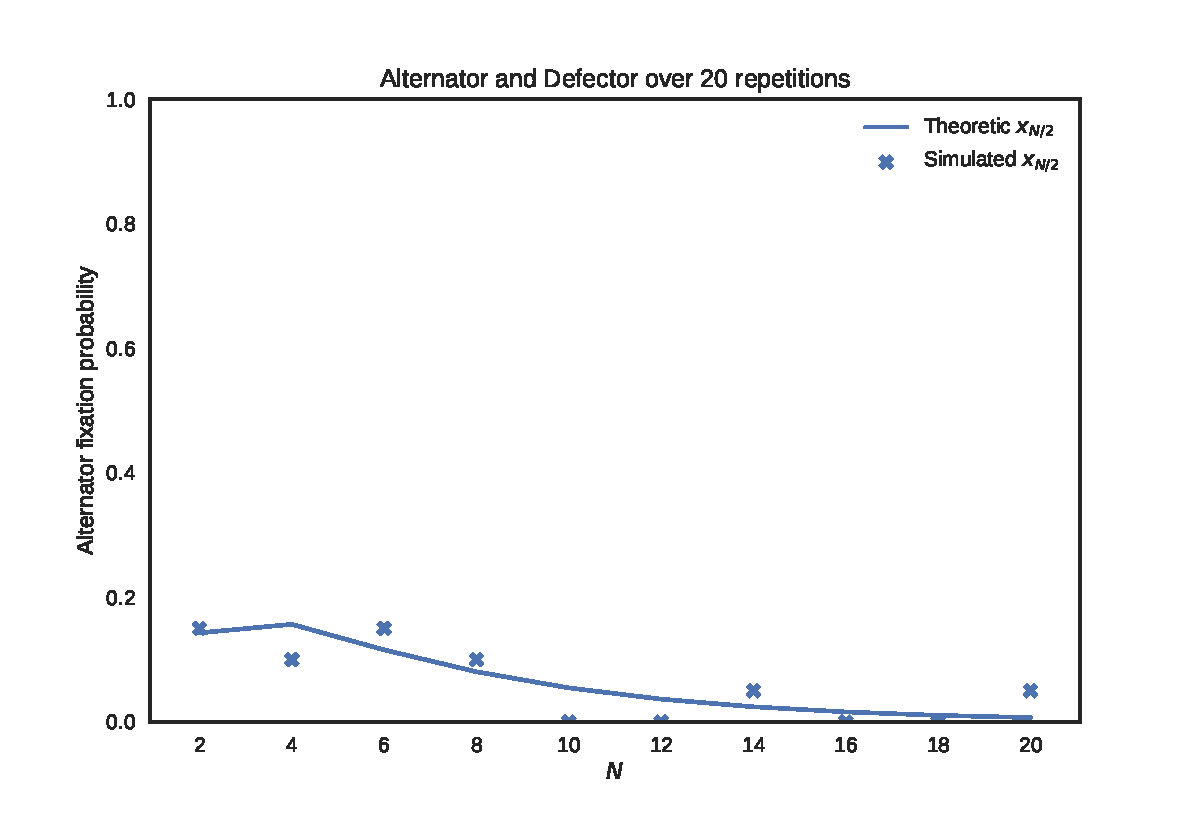
\includegraphics[width=.8\textwidth]{../img/Alternator_v_Defector.pdf}
        \caption{Alternator and Defector}
    \end{subfigure}%
    ~
    \begin{subfigure}[t]{.3\textwidth}
        \centering
        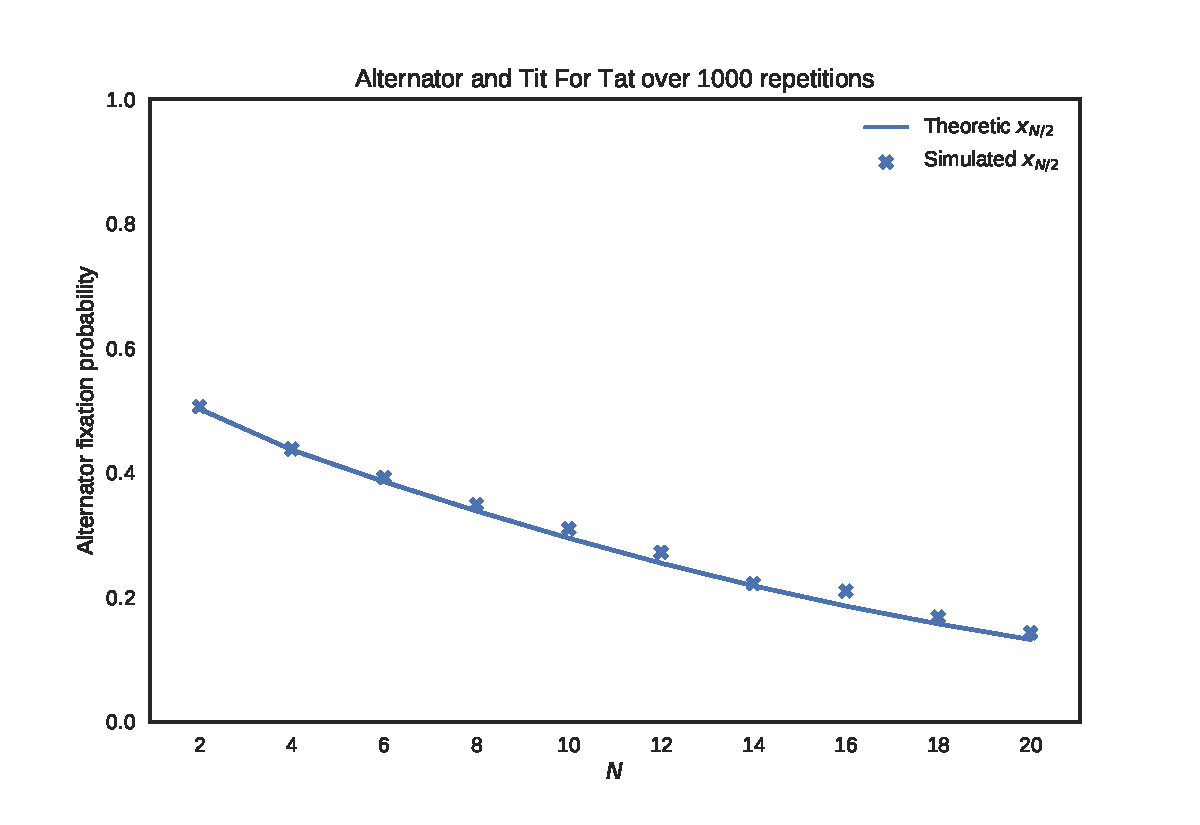
\includegraphics[width=.8\textwidth]{../img/Alternator_v_Tit_For_Tat.pdf}
        \caption{Alternator and Tit For Tat}
    \end{subfigure}%

    \begin{subfigure}[t]{.3\textwidth}
        \centering
        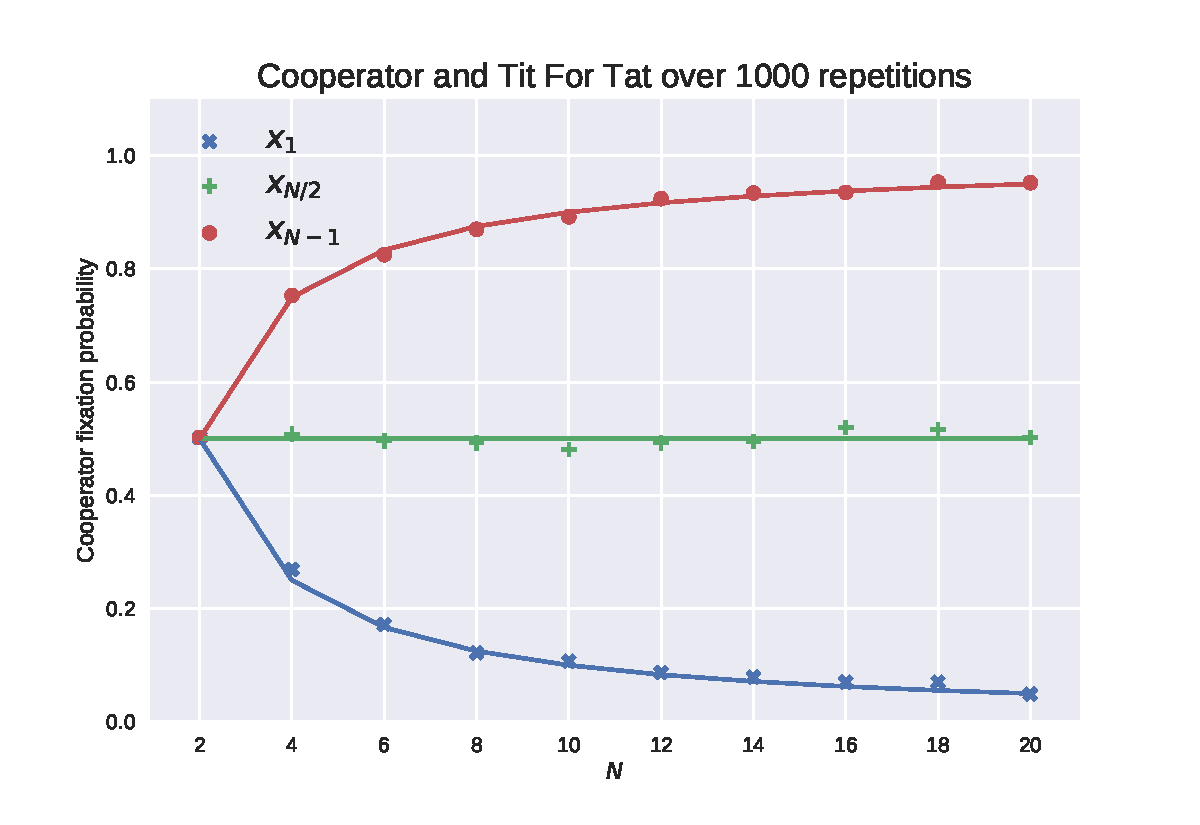
\includegraphics[width=.8\textwidth]{../img/Cooperator_v_Tit_For_Tat.pdf}
        \caption{Cooperator and Tit For Tat}
    \end{subfigure}%
    ~
    \begin{subfigure}[t]{.3\textwidth}
        \centering
        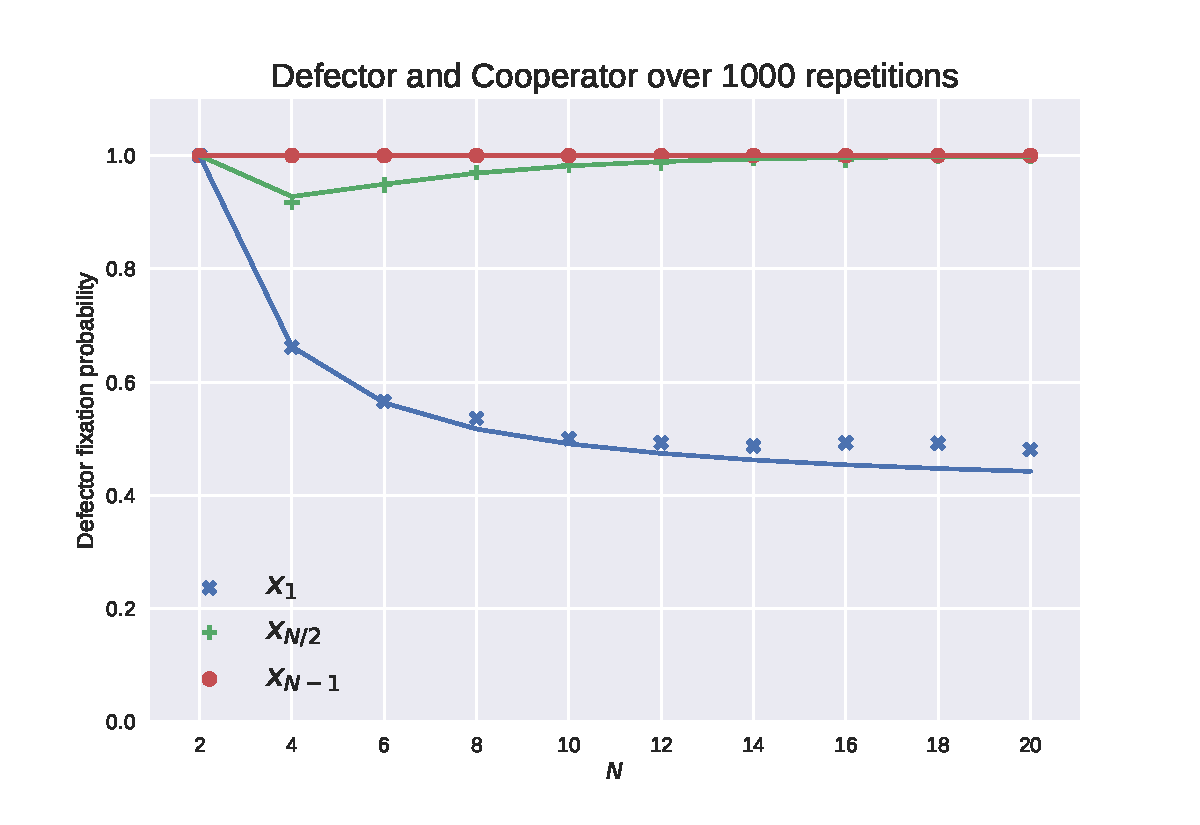
\includegraphics[width=.8\textwidth]{../img/Defector_v_Cooperator.pdf}
        \caption{Defector and Cooperator}
    \end{subfigure}%
    ~
    \begin{subfigure}[t]{.3\textwidth}
        \centering
        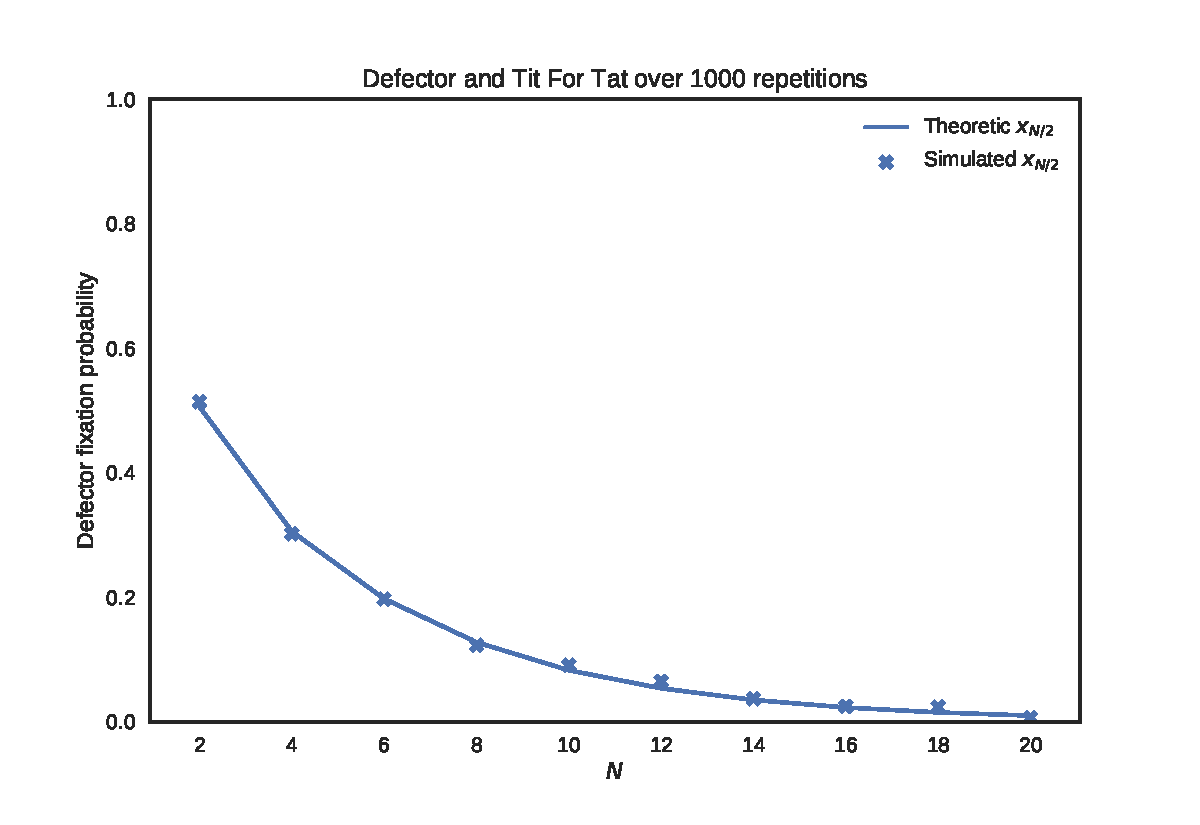
\includegraphics[width=.8\textwidth]{../img/Defector_v_Tit_For_Tat.pdf}
        \caption{Defector and Tit For Tat}
    \end{subfigure}%

    \begin{subfigure}[t]{.3\textwidth}
        \centering
        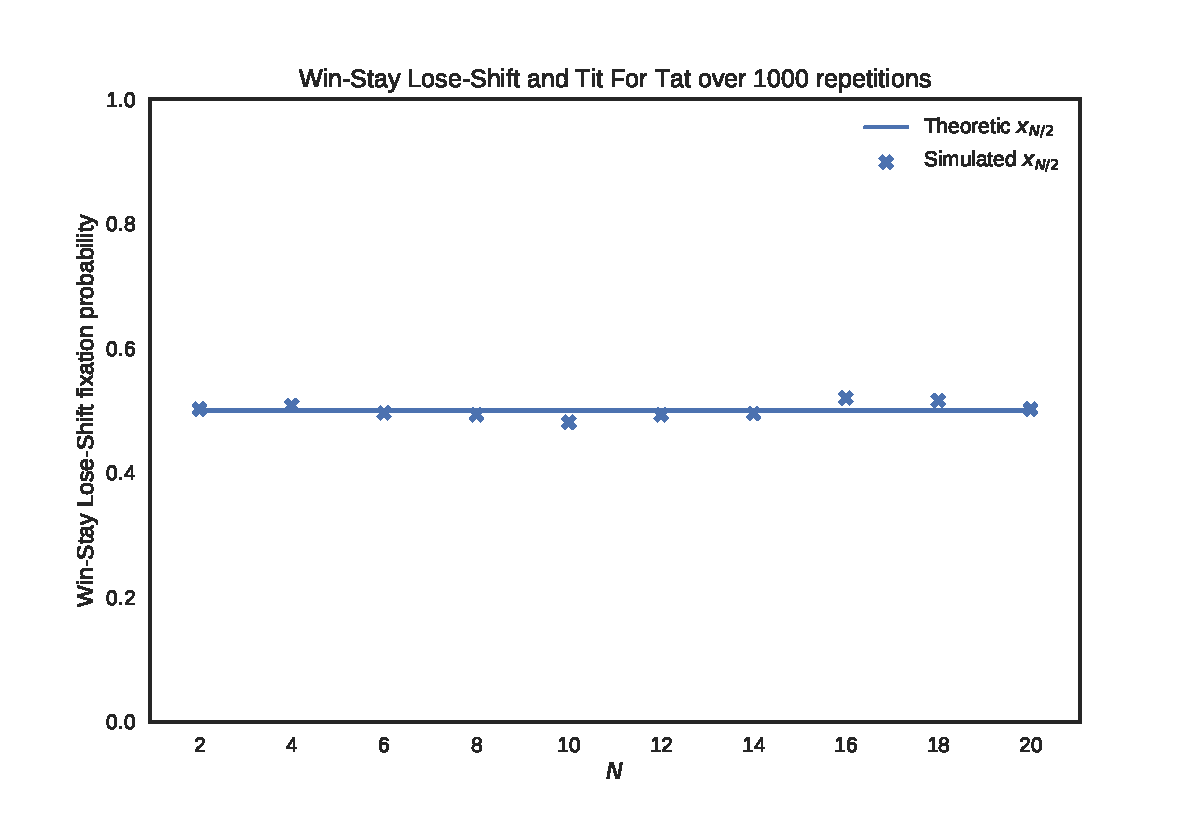
\includegraphics[width=.8\textwidth]{../img/Win-Stay_Lose-Shift_v_Tit_For_Tat.pdf}
        \caption{Win Stay Lose Shift and Tit For Tat}
    \end{subfigure}%
    ~
    \begin{subfigure}[t]{.3\textwidth}
        \centering
        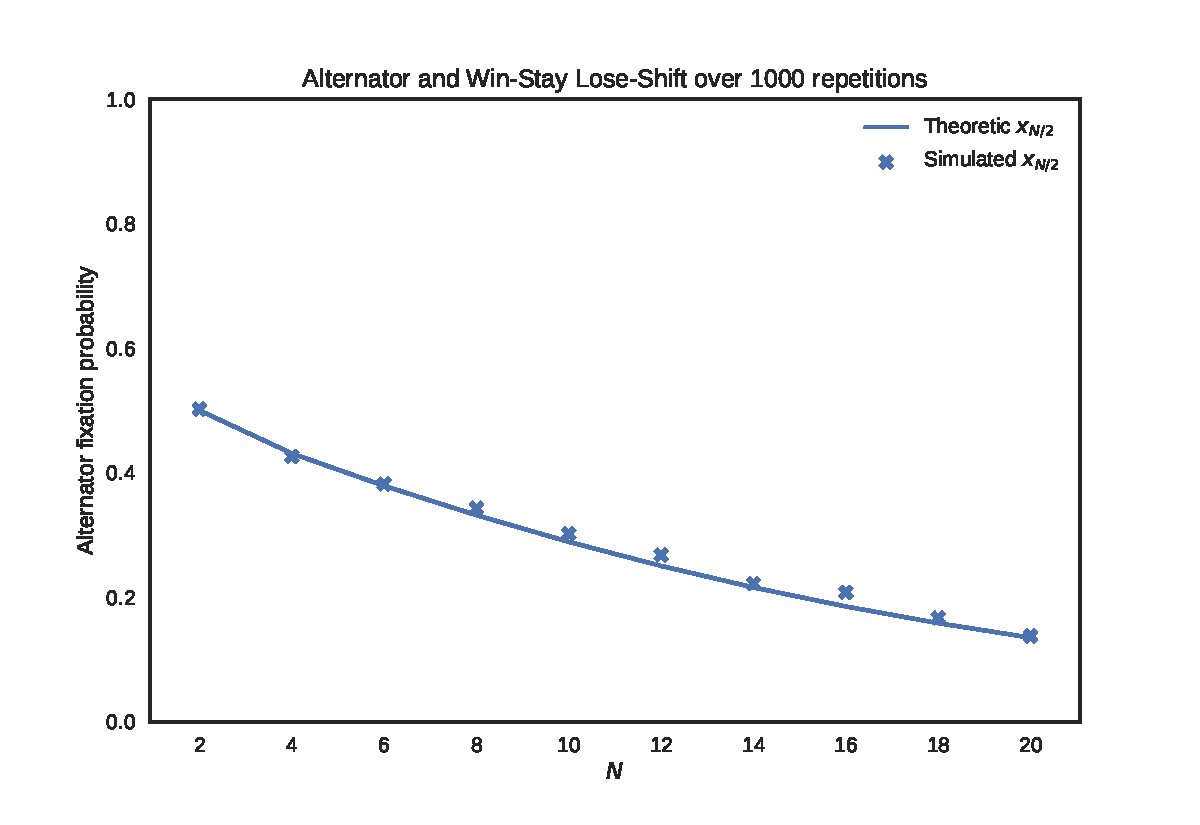
\includegraphics[width=.8\textwidth]{../img/Alternator_v_Win-Stay_Lose-Shift.pdf}
        \caption{Alternator and Win Stay Lose Shift}
    \end{subfigure}%
    ~
    \begin{subfigure}[t]{.3\textwidth}
        \centering
        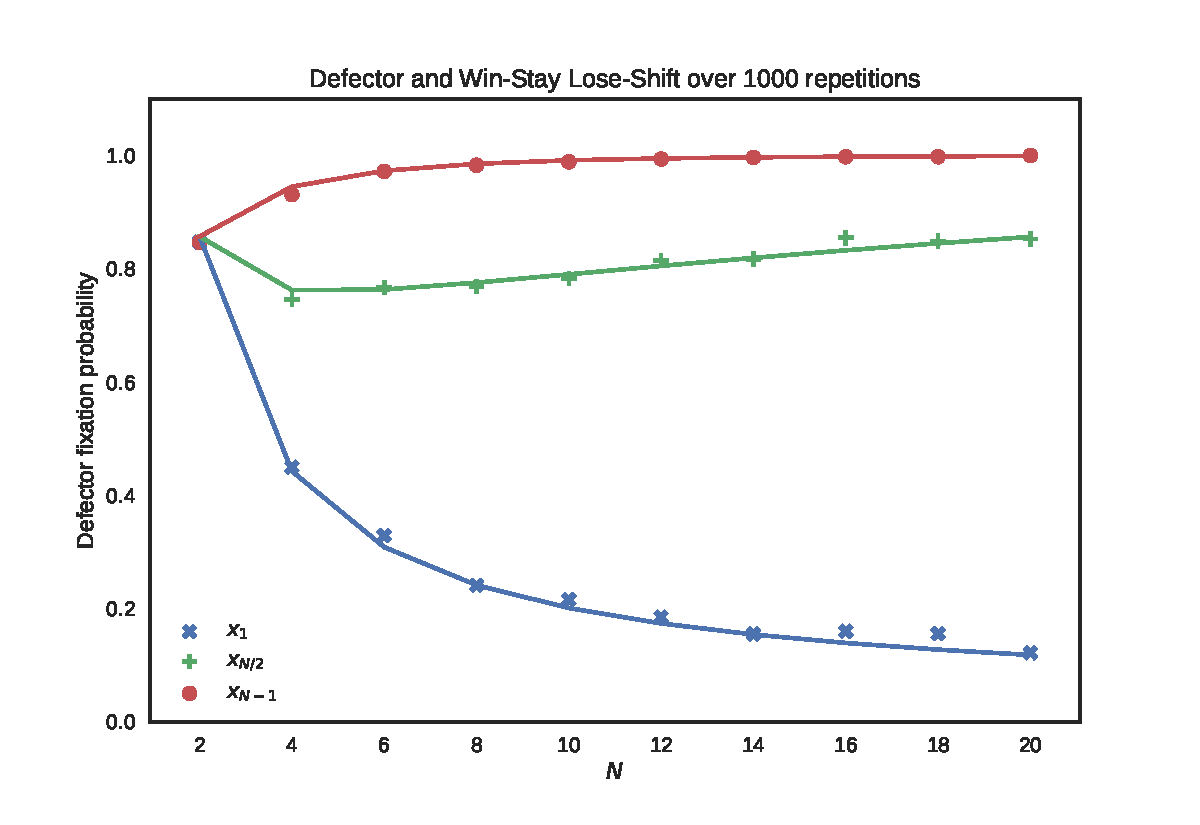
\includegraphics[width=.8\textwidth]{../img/Defector_v_Win-Stay_Lose-Shift.pdf}
        \caption{Defector and Win Stay Lose Shift}
    \end{subfigure}%
    \caption{Comparison of theoretic and actual Moran Process fixation
             probabilities for \textbf{deterministic} strategies}
    \label{fig:comparison_deterministic}
\end{figure}

\begin{figure}[!hbtp]
    \centering
    \begin{subfigure}[t]{.3\textwidth}
        \centering
        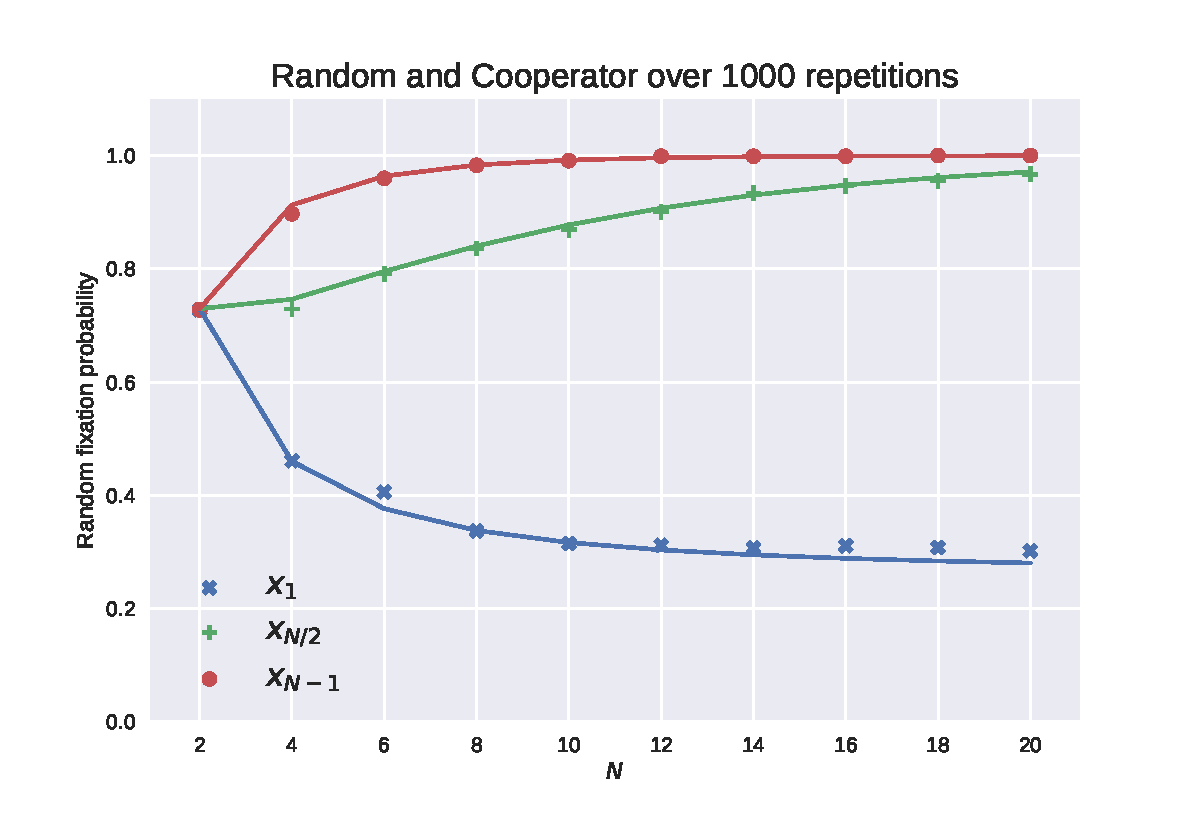
\includegraphics[width=.8\textwidth]{../img/Random_v_Cooperator.pdf}
        \caption{Random and Cooperator}
    \end{subfigure}%
    ~
    \begin{subfigure}[t]{.3\textwidth}
        \centering
        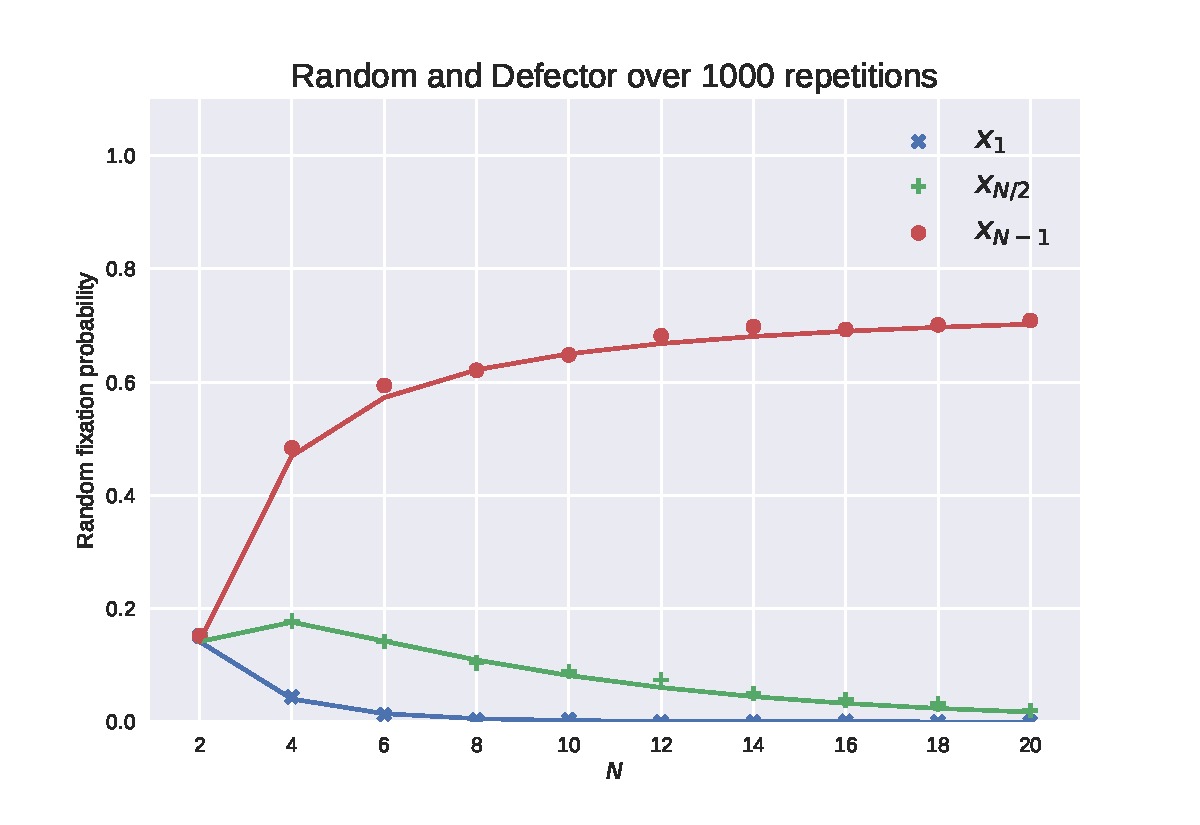
\includegraphics[width=.8\textwidth]{../img/Random_v_Defector.pdf}
        \caption{Random and Defector}
    \end{subfigure}%
    ~
    \begin{subfigure}[t]{.3\textwidth}
        \centering
        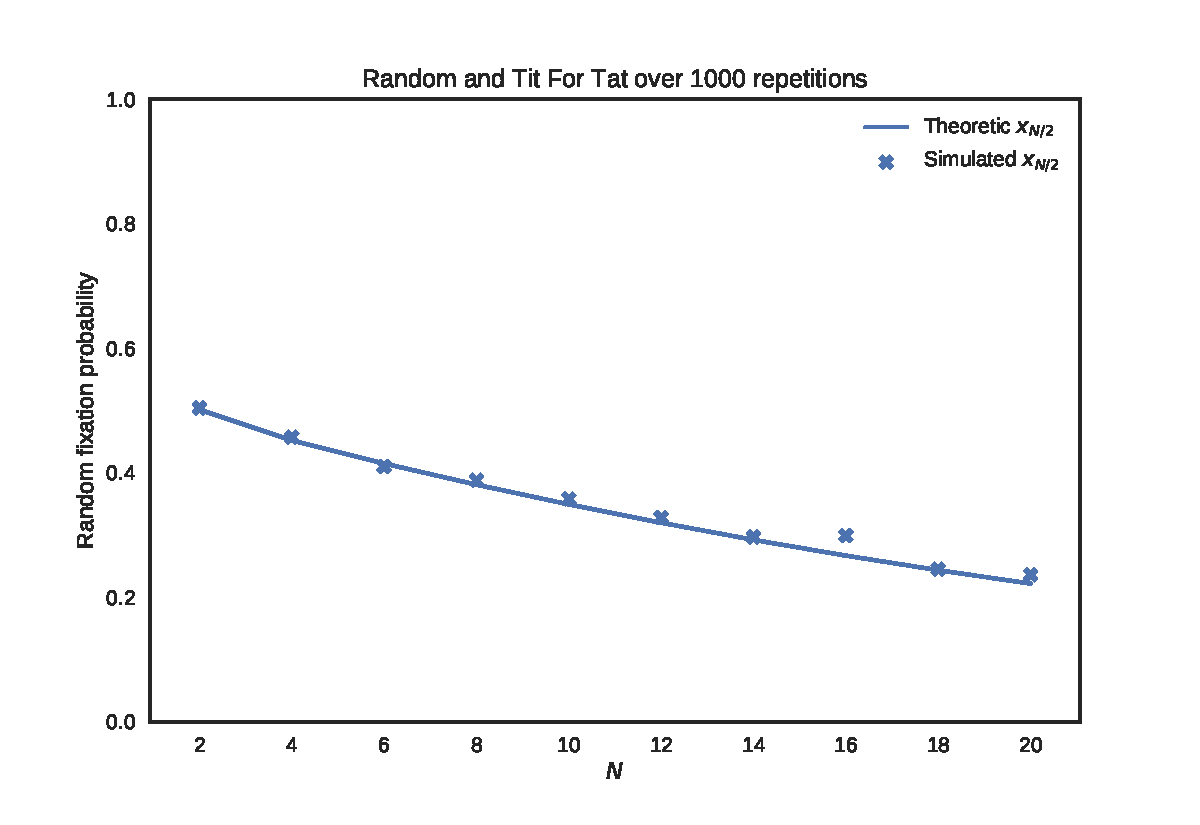
\includegraphics[width=.8\textwidth]{../img/Random_v_Tit_For_Tat.pdf}
        \caption{Random and Tit For Tat}
    \end{subfigure}%

    \begin{subfigure}[t]{.3\textwidth}
        \centering
        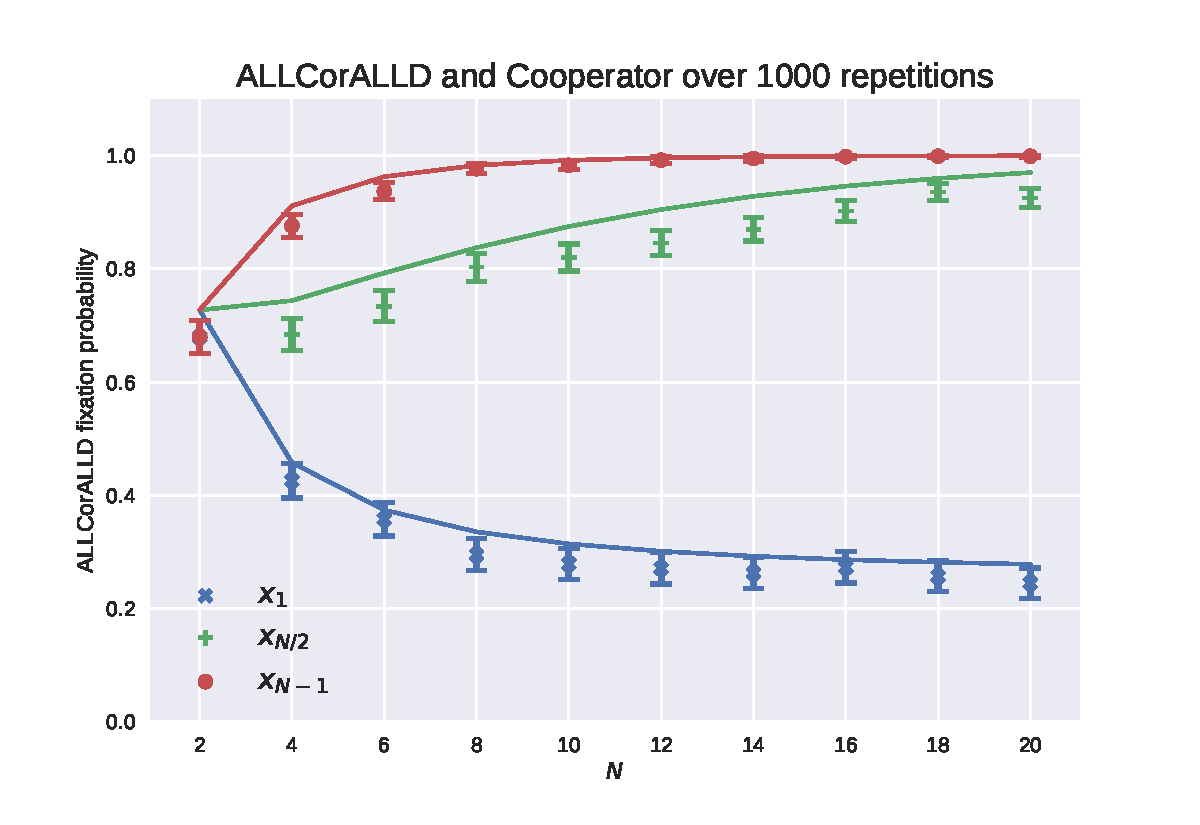
\includegraphics[width=.8\textwidth]{../img/ALLCorALLD_v_Cooperator.pdf}
        \caption{All C or all D and Cooperator}
    \end{subfigure}%
    ~
    \begin{subfigure}[t]{.3\textwidth}
        \centering
        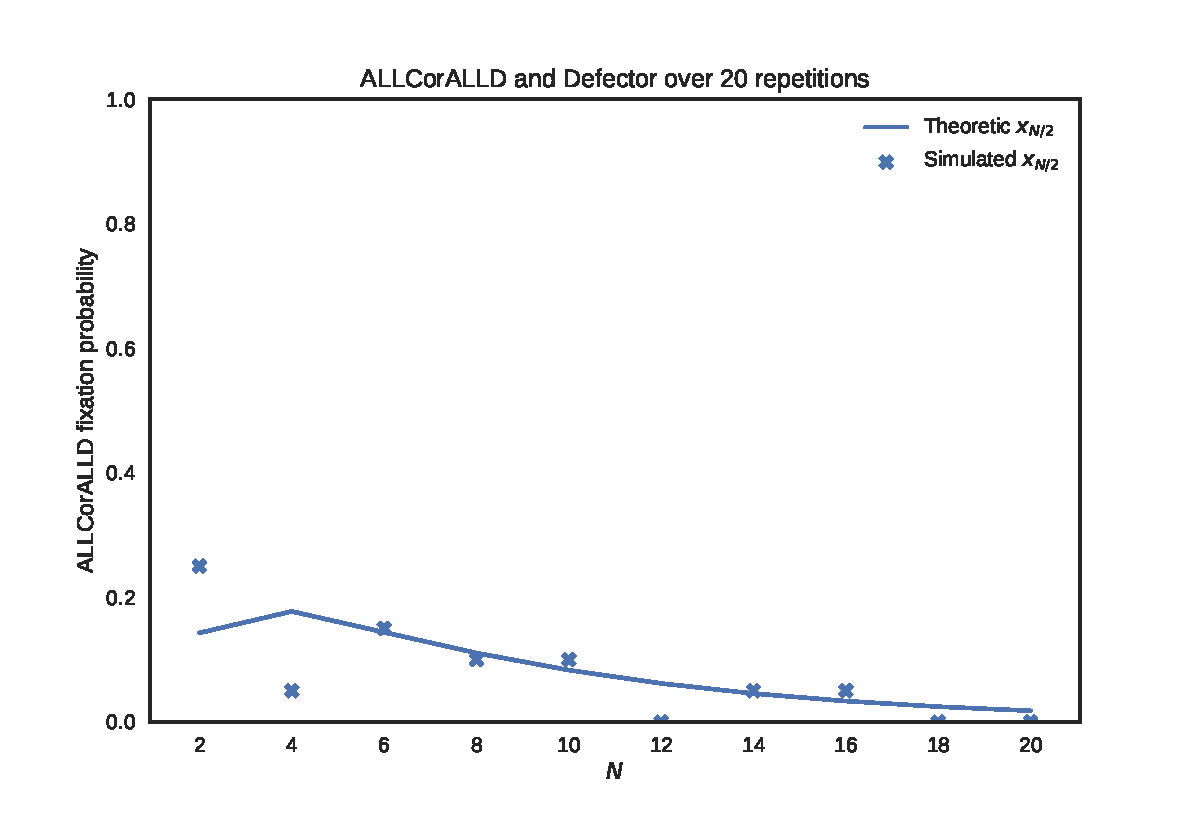
\includegraphics[width=.8\textwidth]{../img/ALLCorALLD_v_Defector.pdf}
        \caption{All C or all D and Defector}
    \end{subfigure}%
    ~
    \begin{subfigure}[t]{.3\textwidth}
        \centering
        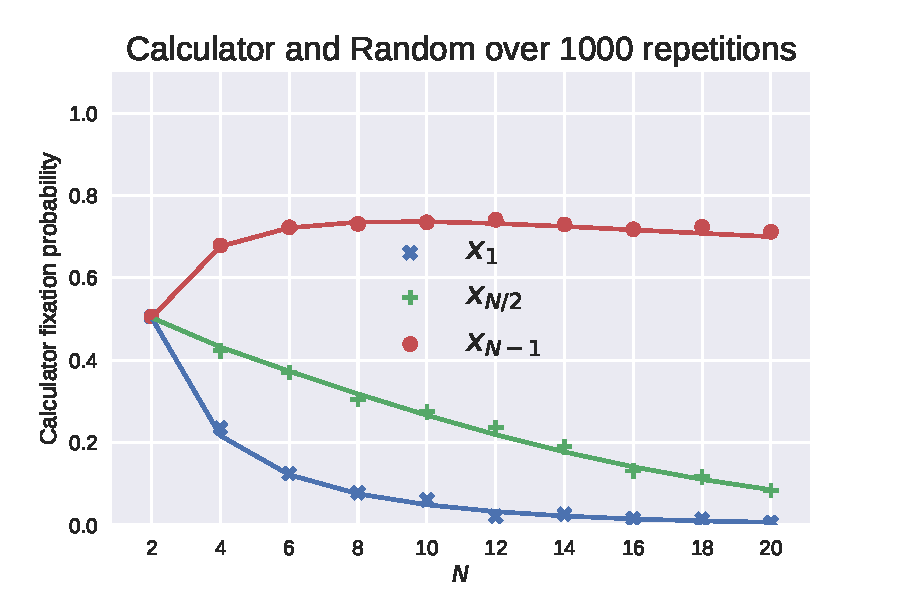
\includegraphics[width=.8\textwidth]{../img/Calculator_v_Random.pdf}
        \caption{Calculator and Random}
    \end{subfigure}%

    \begin{subfigure}[t]{.3\textwidth}
        \centering
        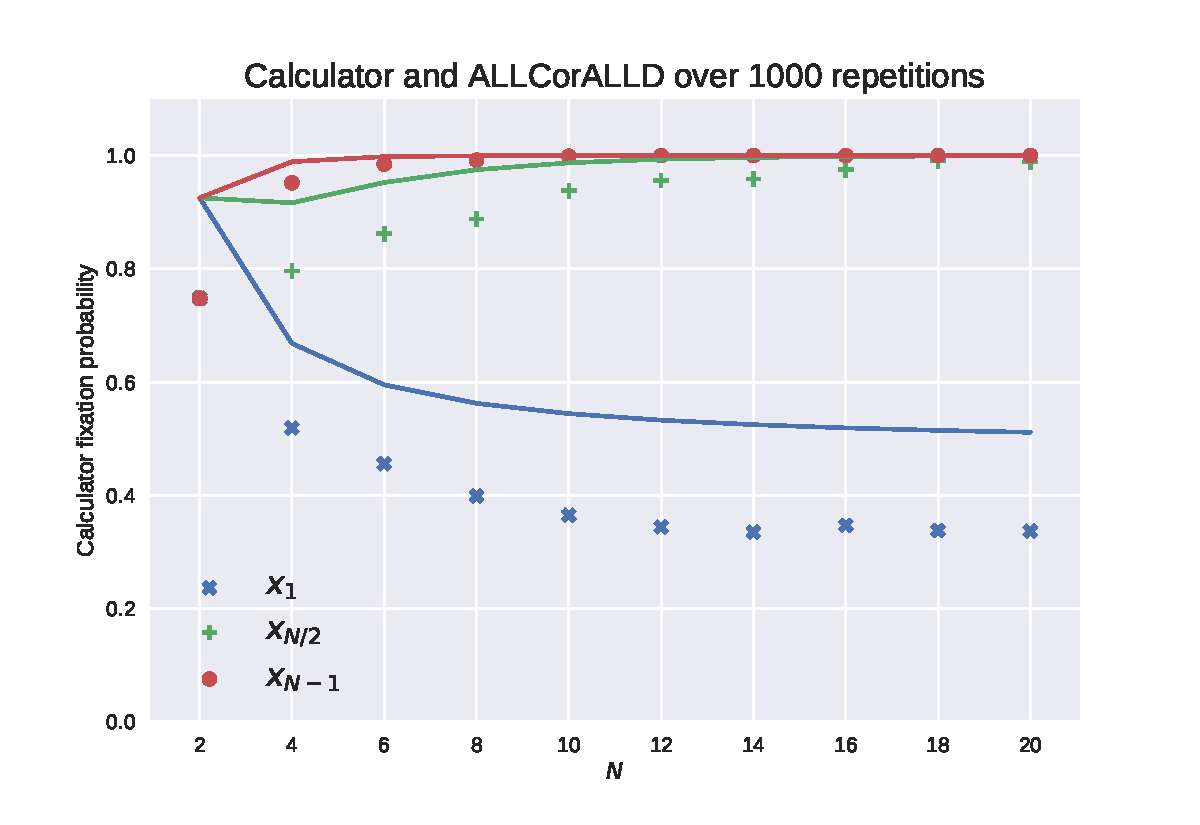
\includegraphics[width=.8\textwidth]{../img/Calculator_v_ALLCorALLD.pdf}
        \caption{Calculator and All C or all D}
    \end{subfigure}%
    ~
    \begin{subfigure}[t]{.3\textwidth}
        \centering
        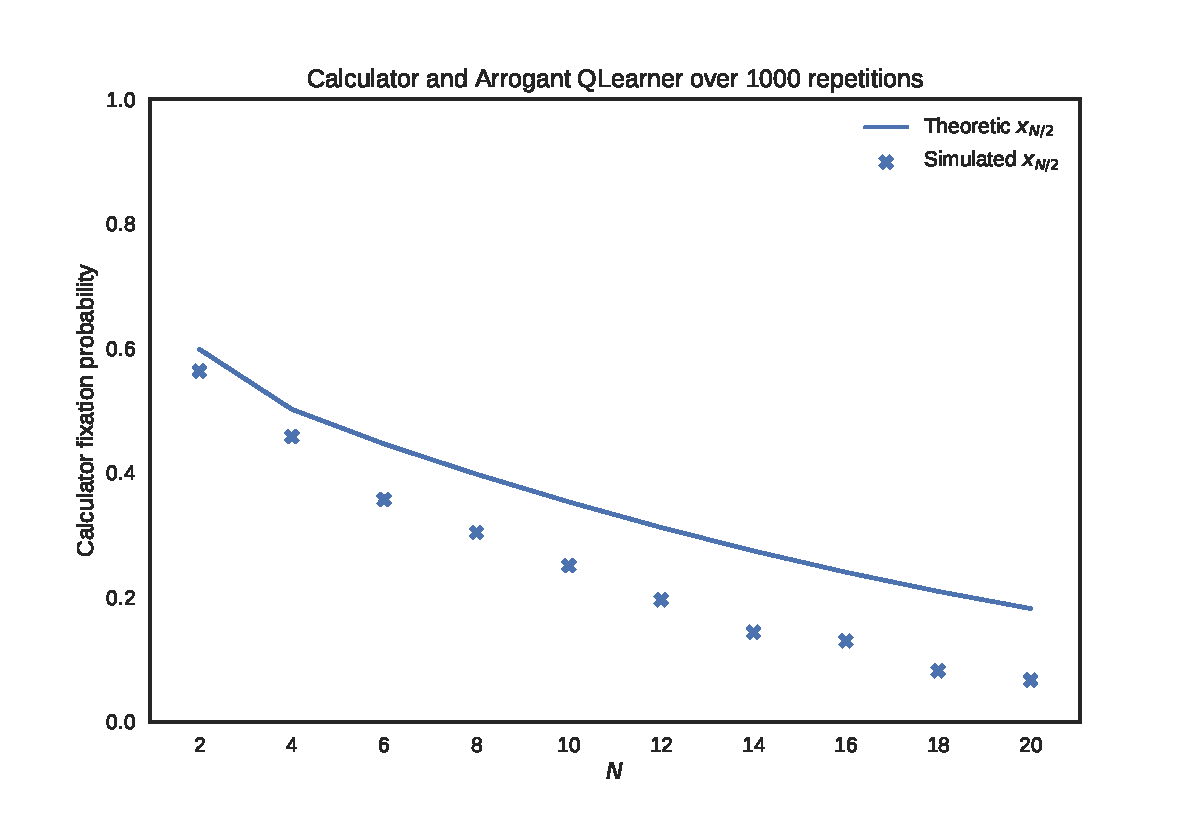
\includegraphics[width=.8\textwidth]{../img/Calculator_v_Arrogant_QLearner.pdf}
        \caption{Calculator and Arrogant Q learner}
    \end{subfigure}%
    ~
    \begin{subfigure}[t]{.3\textwidth}
        \centering
        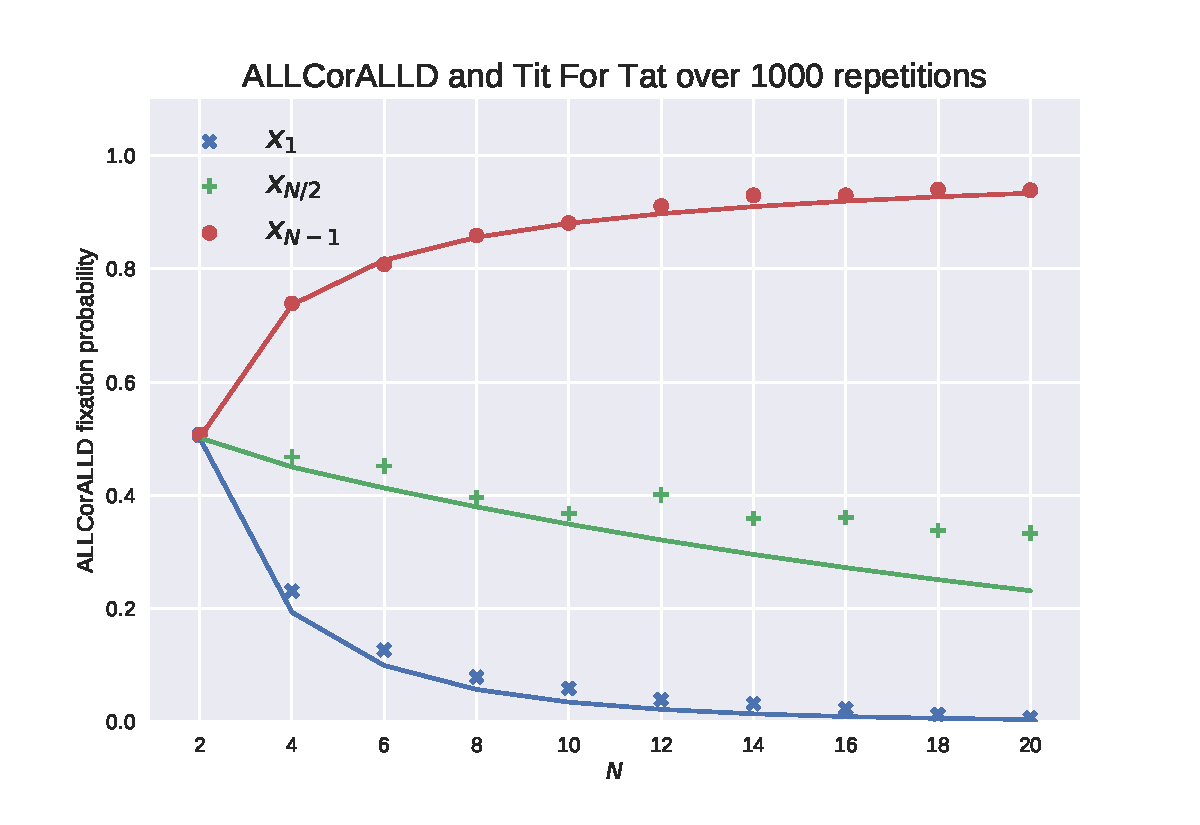
\includegraphics[width=.8\textwidth]{../img/ALLCorALLD_v_Tit_For_Tat.pdf}
        \caption{All C or all D and Tit For Tat}
    \end{subfigure}%
    \caption{Comparison of theoretic and actual Moran Process
             fixation probabilities for \textbf{stochastic} strategies}
    \label{fig:comparison_stochastic}
\end{figure}

Figure~\ref{fig:comparison_stochastic} shows the fixation probabilities for
stochastic strategies. These are no longer a good match which highlights the
weakness of the analytical formulae that relies on the average payoffs. A
detailed analysis of the 172 strategies considered will be shown in the next
Section.

\section{Numerical results}\label{sec:numerical_results}

Figures~\ref{fig:fixation_heatmap_std} and~\ref{fig:fixation_heatmap_noise}
shows the fixation rates of each player on the y axis against each player on the
x axis.

\begin{figure}[!hbtp]
    \centering
    \begin{subfigure}[t]{.3\textwidth}
        \centering
        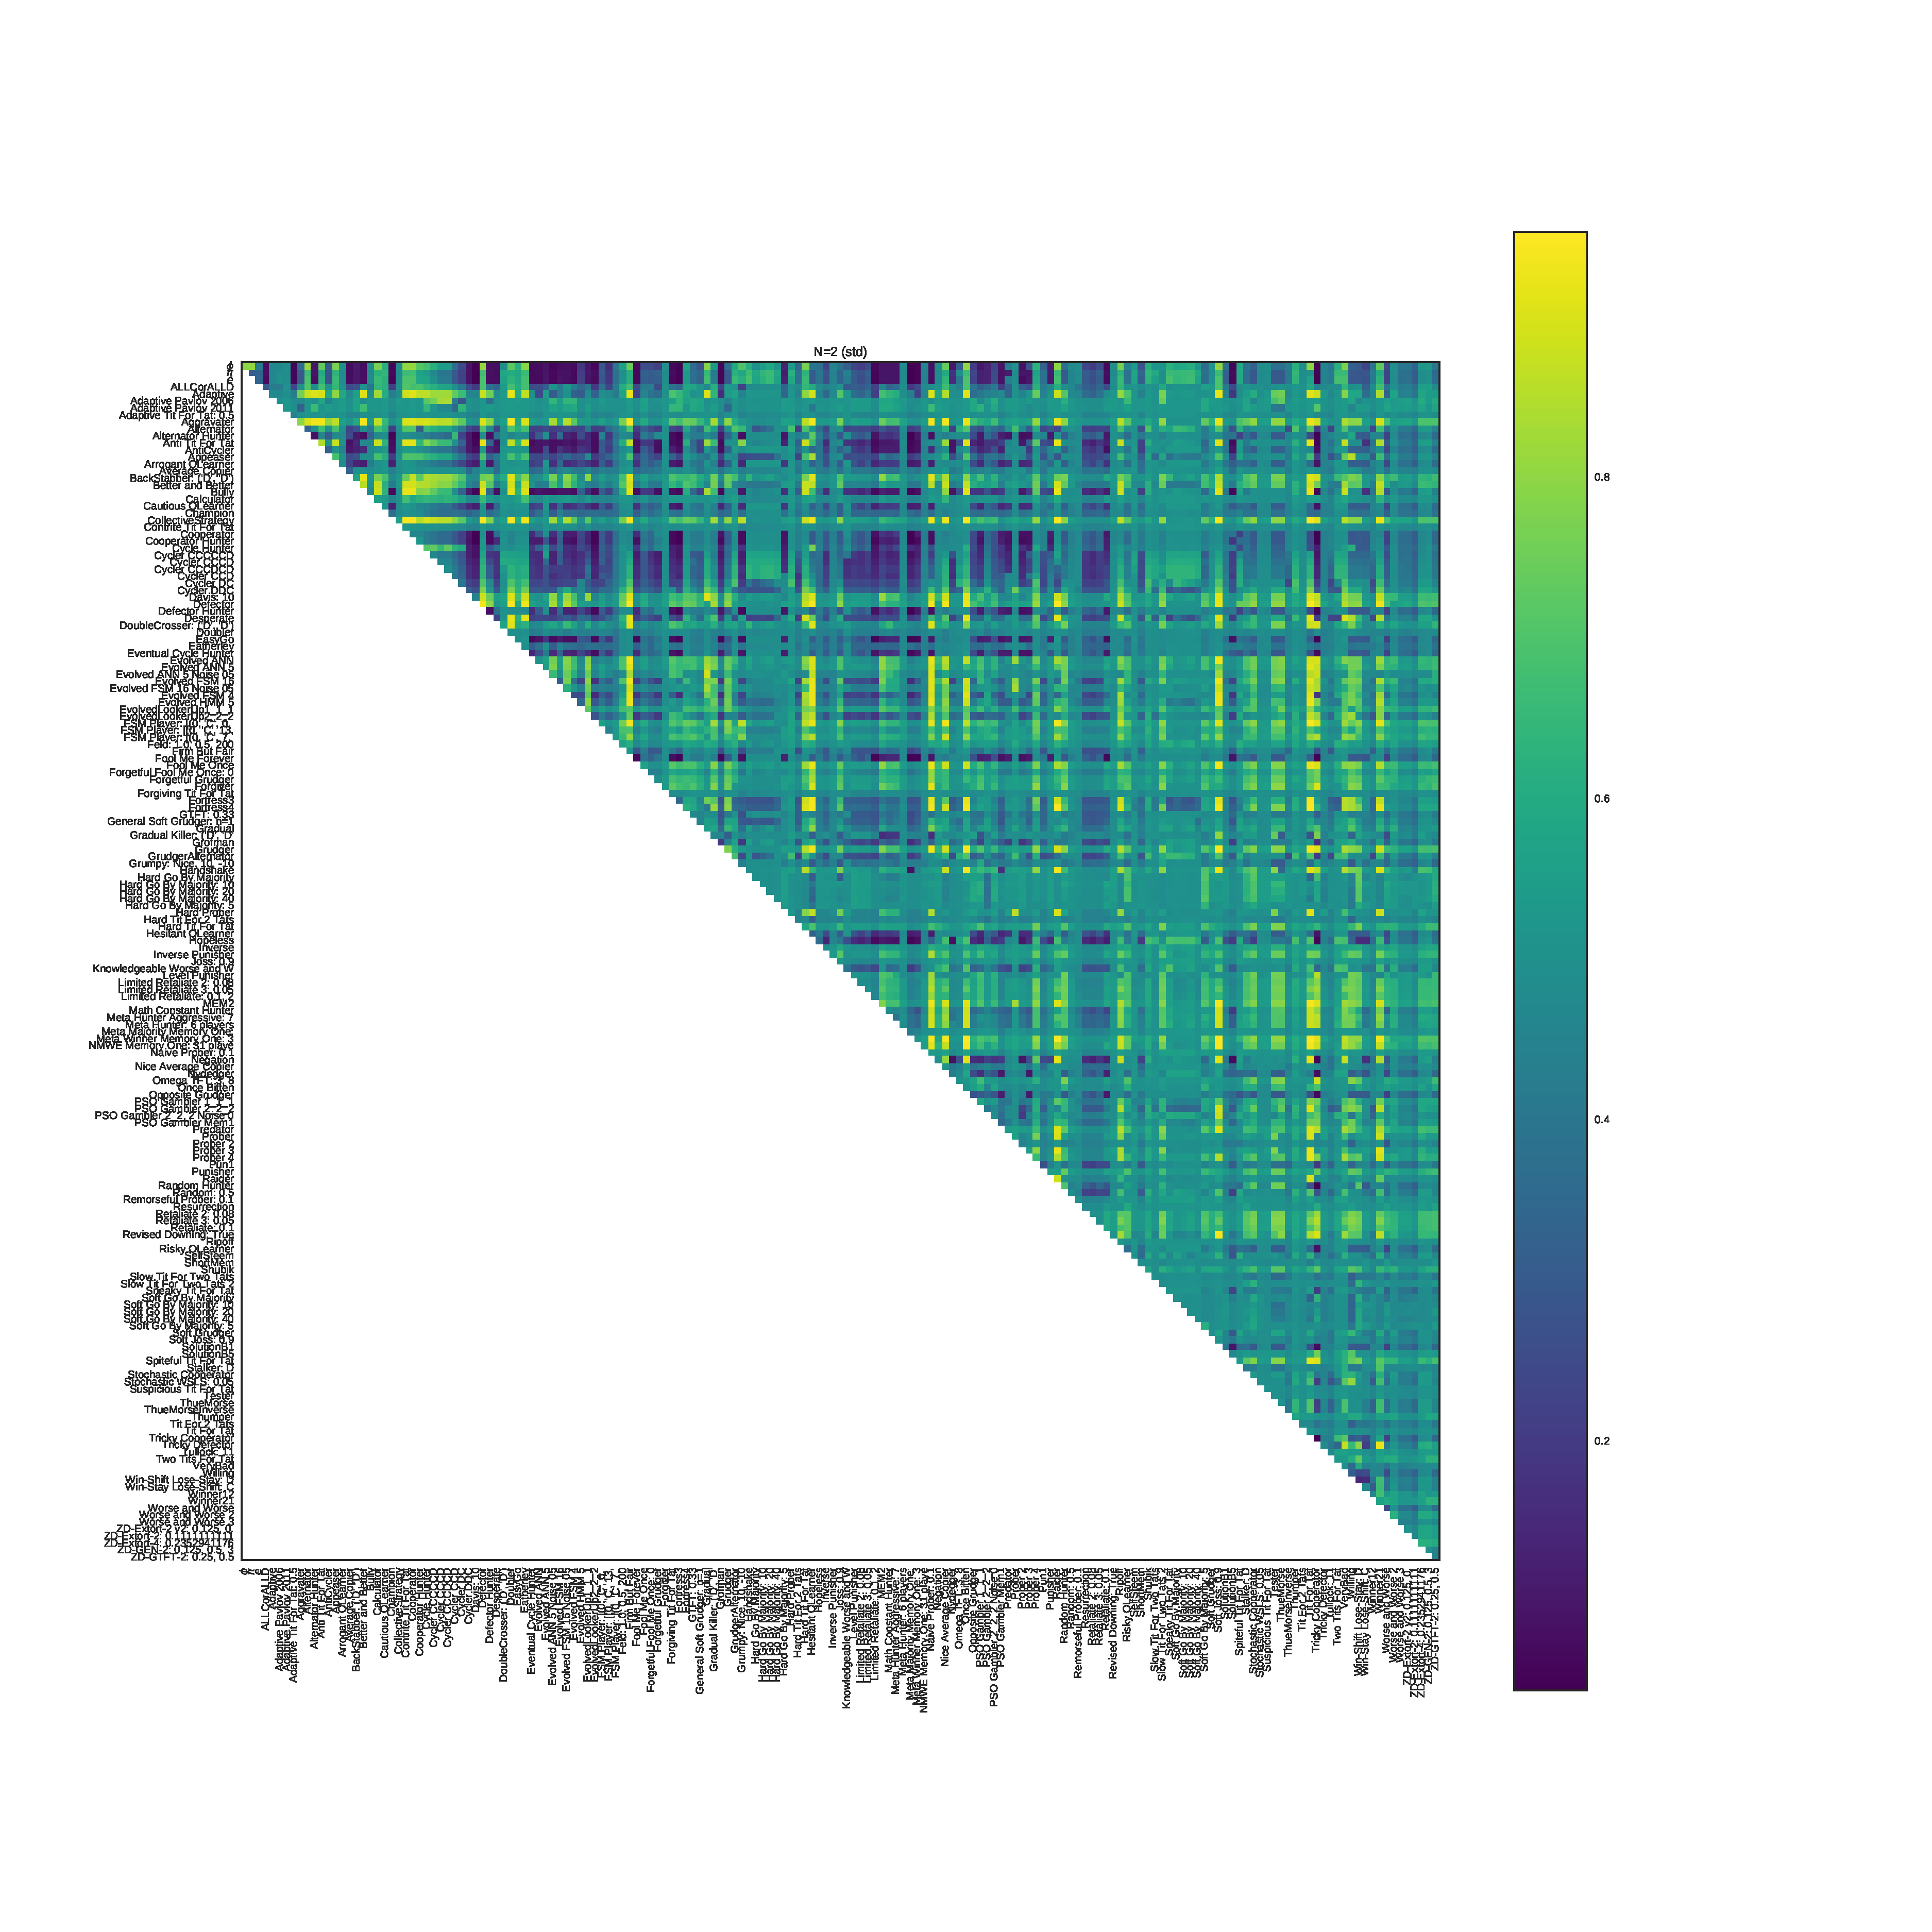
\includegraphics[width=.8\textwidth]{../img/fixation_heatmap_2_std.pdf}
        \caption{\(N=2\)}
    \end{subfigure}%
    ~
    \begin{subfigure}[t]{.3\textwidth}
        \centering
        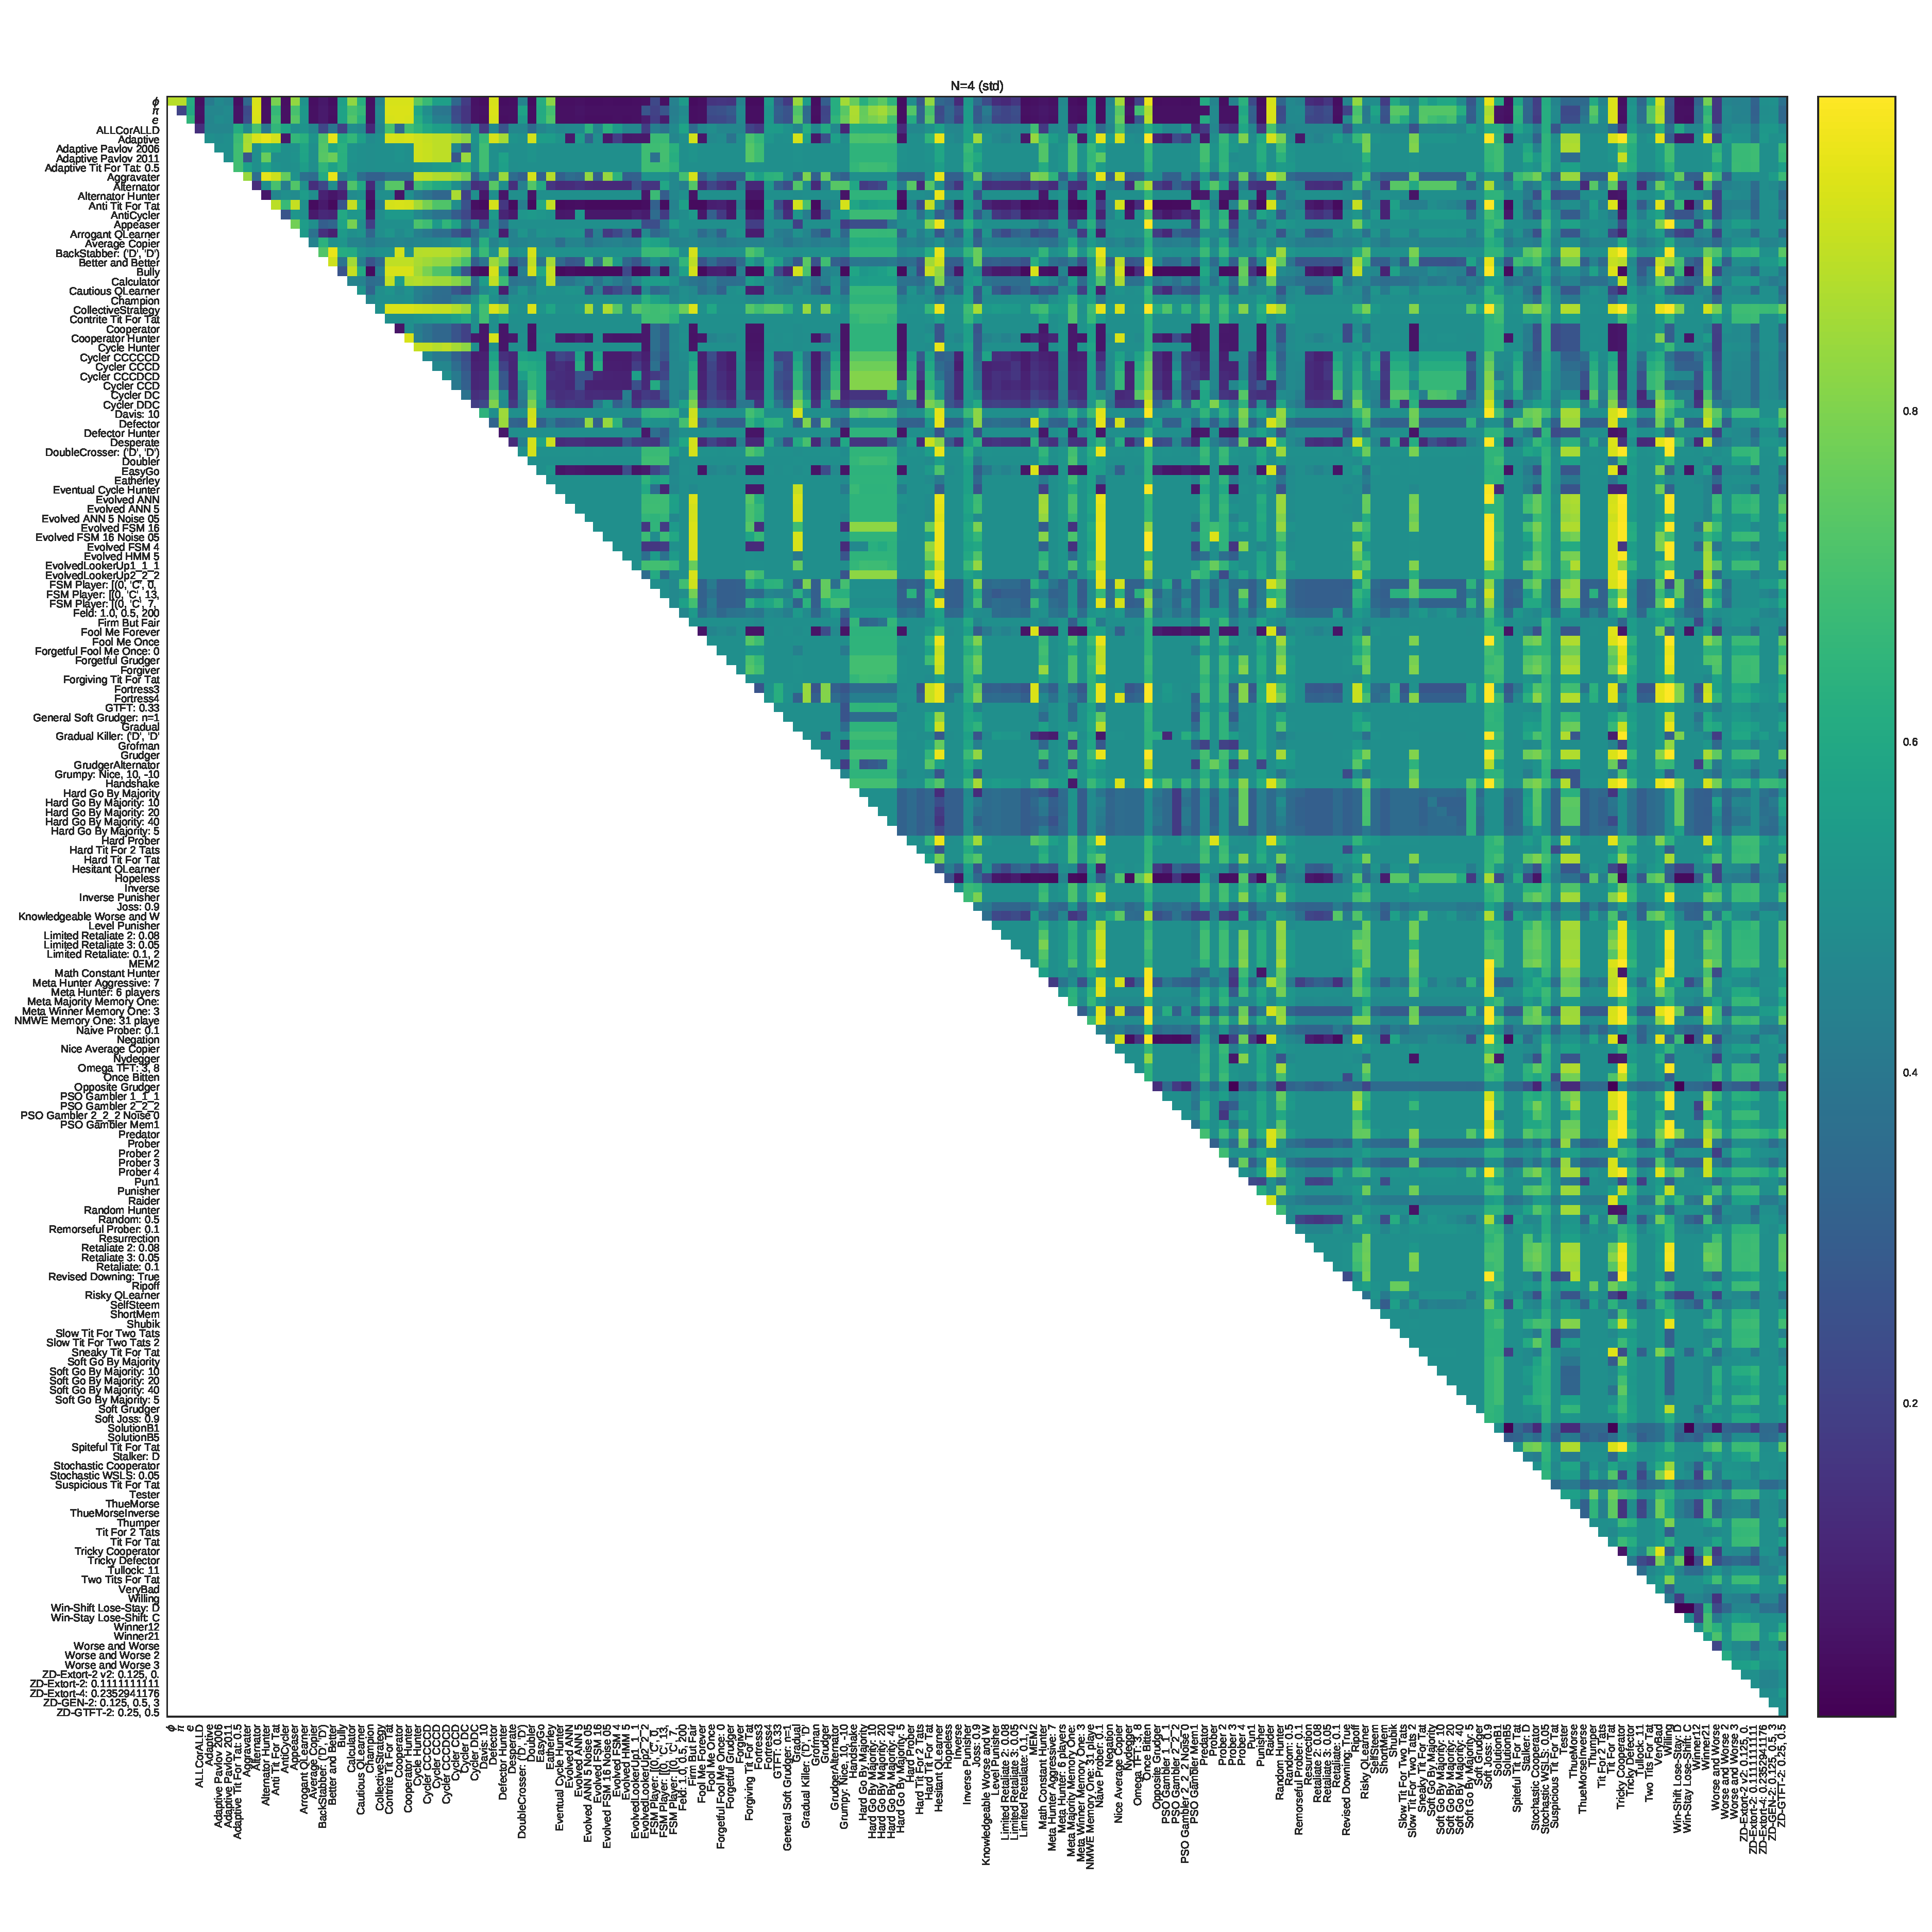
\includegraphics[width=.8\textwidth]{../img/fixation_heatmap_4_std.pdf}
        \caption{\(N=4\)}
    \end{subfigure}%
    ~
    \begin{subfigure}[t]{.3\textwidth}
        \centering
        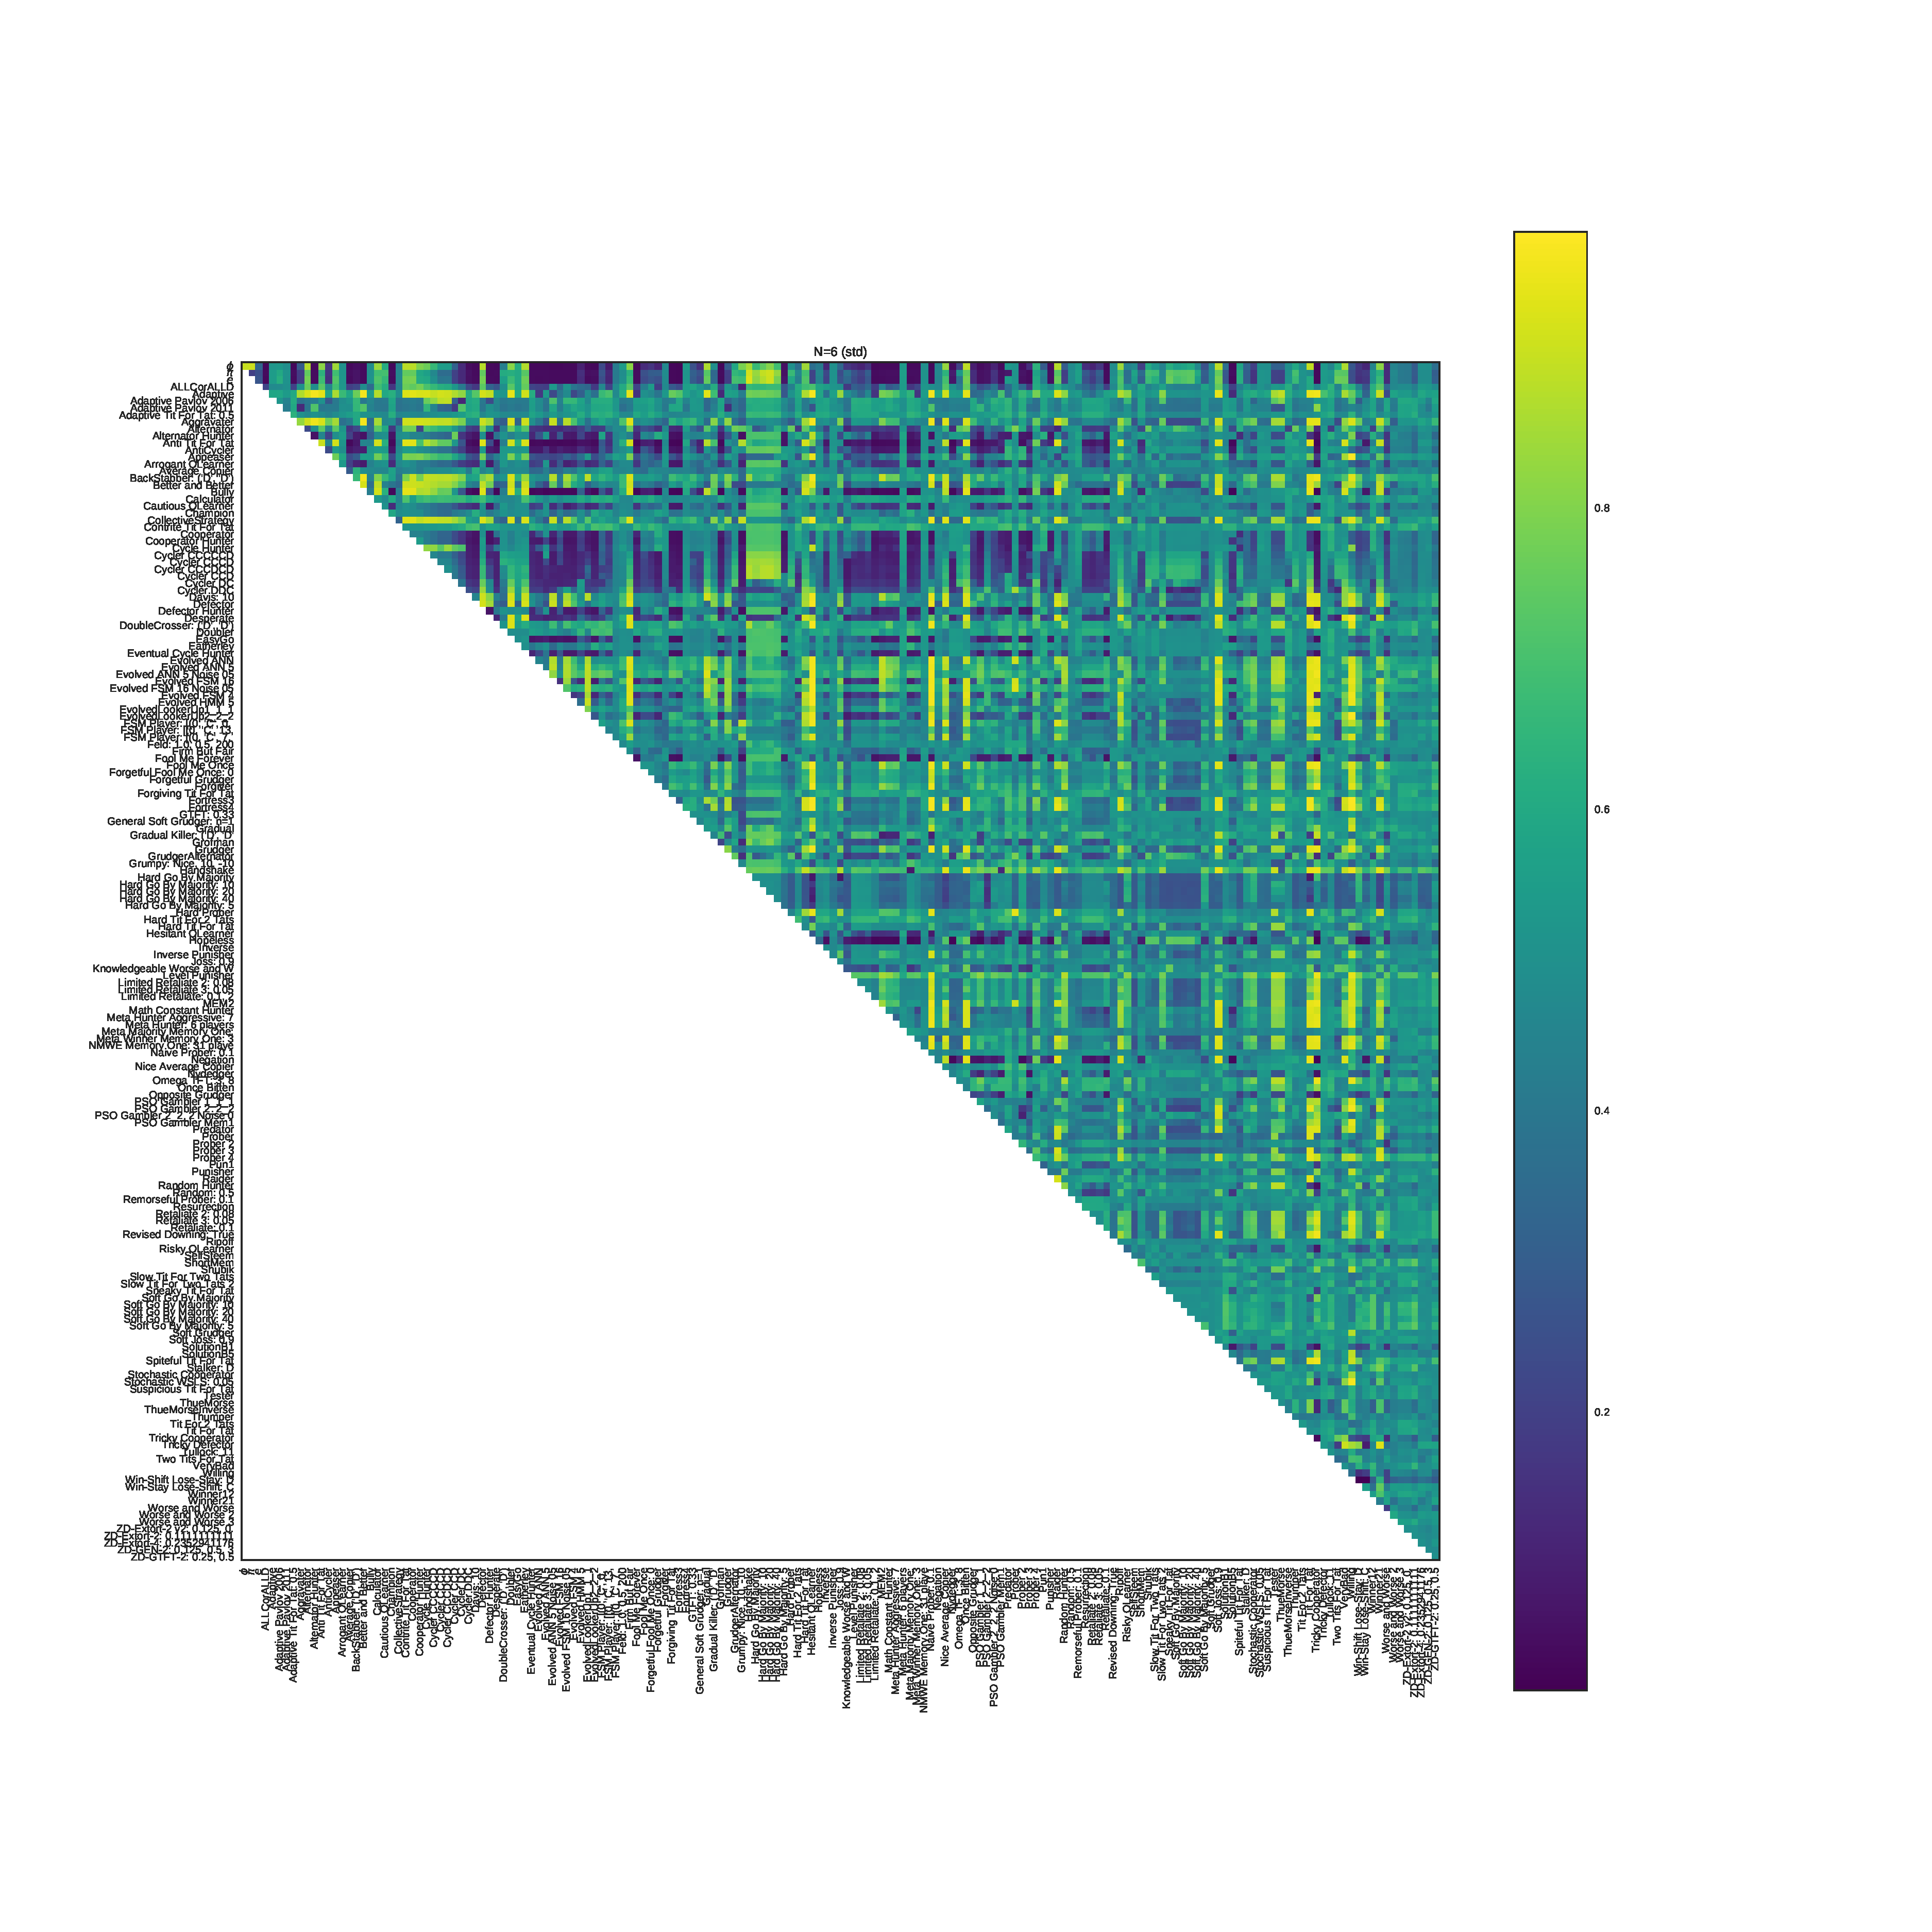
\includegraphics[width=.8\textwidth]{../img/fixation_heatmap_6_std.pdf}
        \caption{\(N=6\)}
    \end{subfigure}%

    \begin{subfigure}[t]{.3\textwidth}
        \centering
        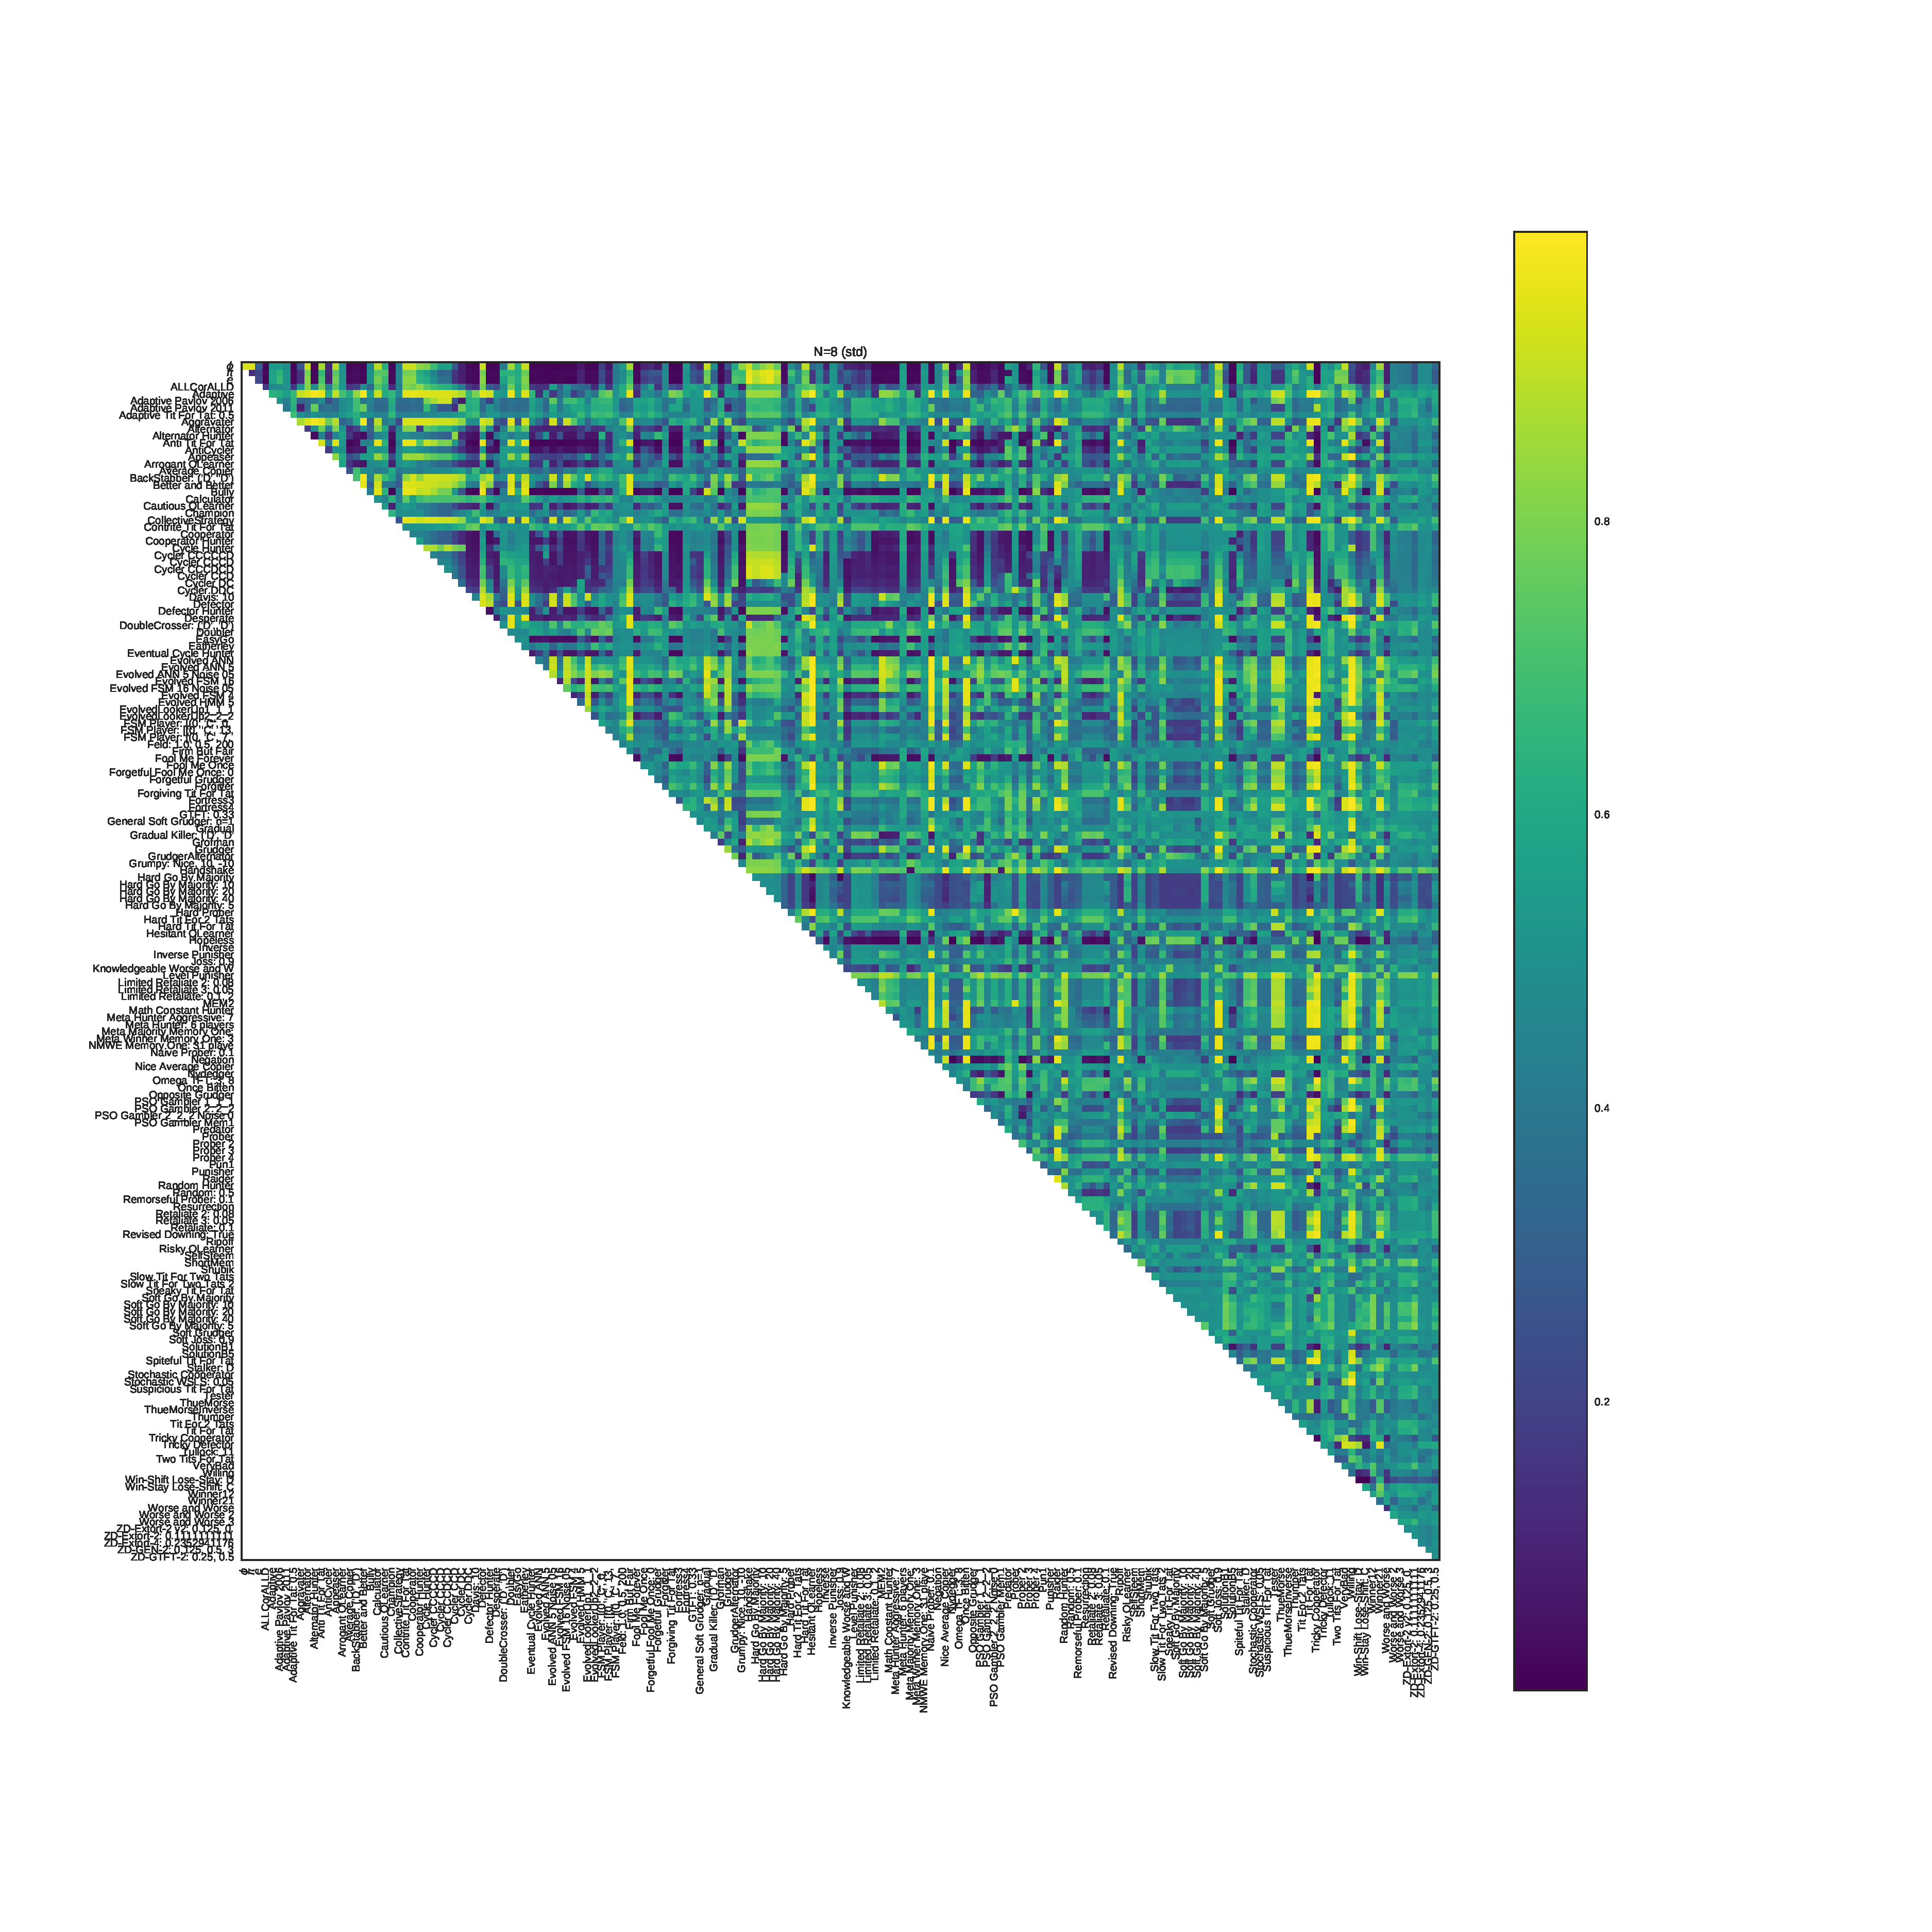
\includegraphics[width=.8\textwidth]{../img/fixation_heatmap_8_std.pdf}
        \caption{\(N=8\)}
    \end{subfigure}%
    ~
    \begin{subfigure}[t]{.3\textwidth}
        \centering
        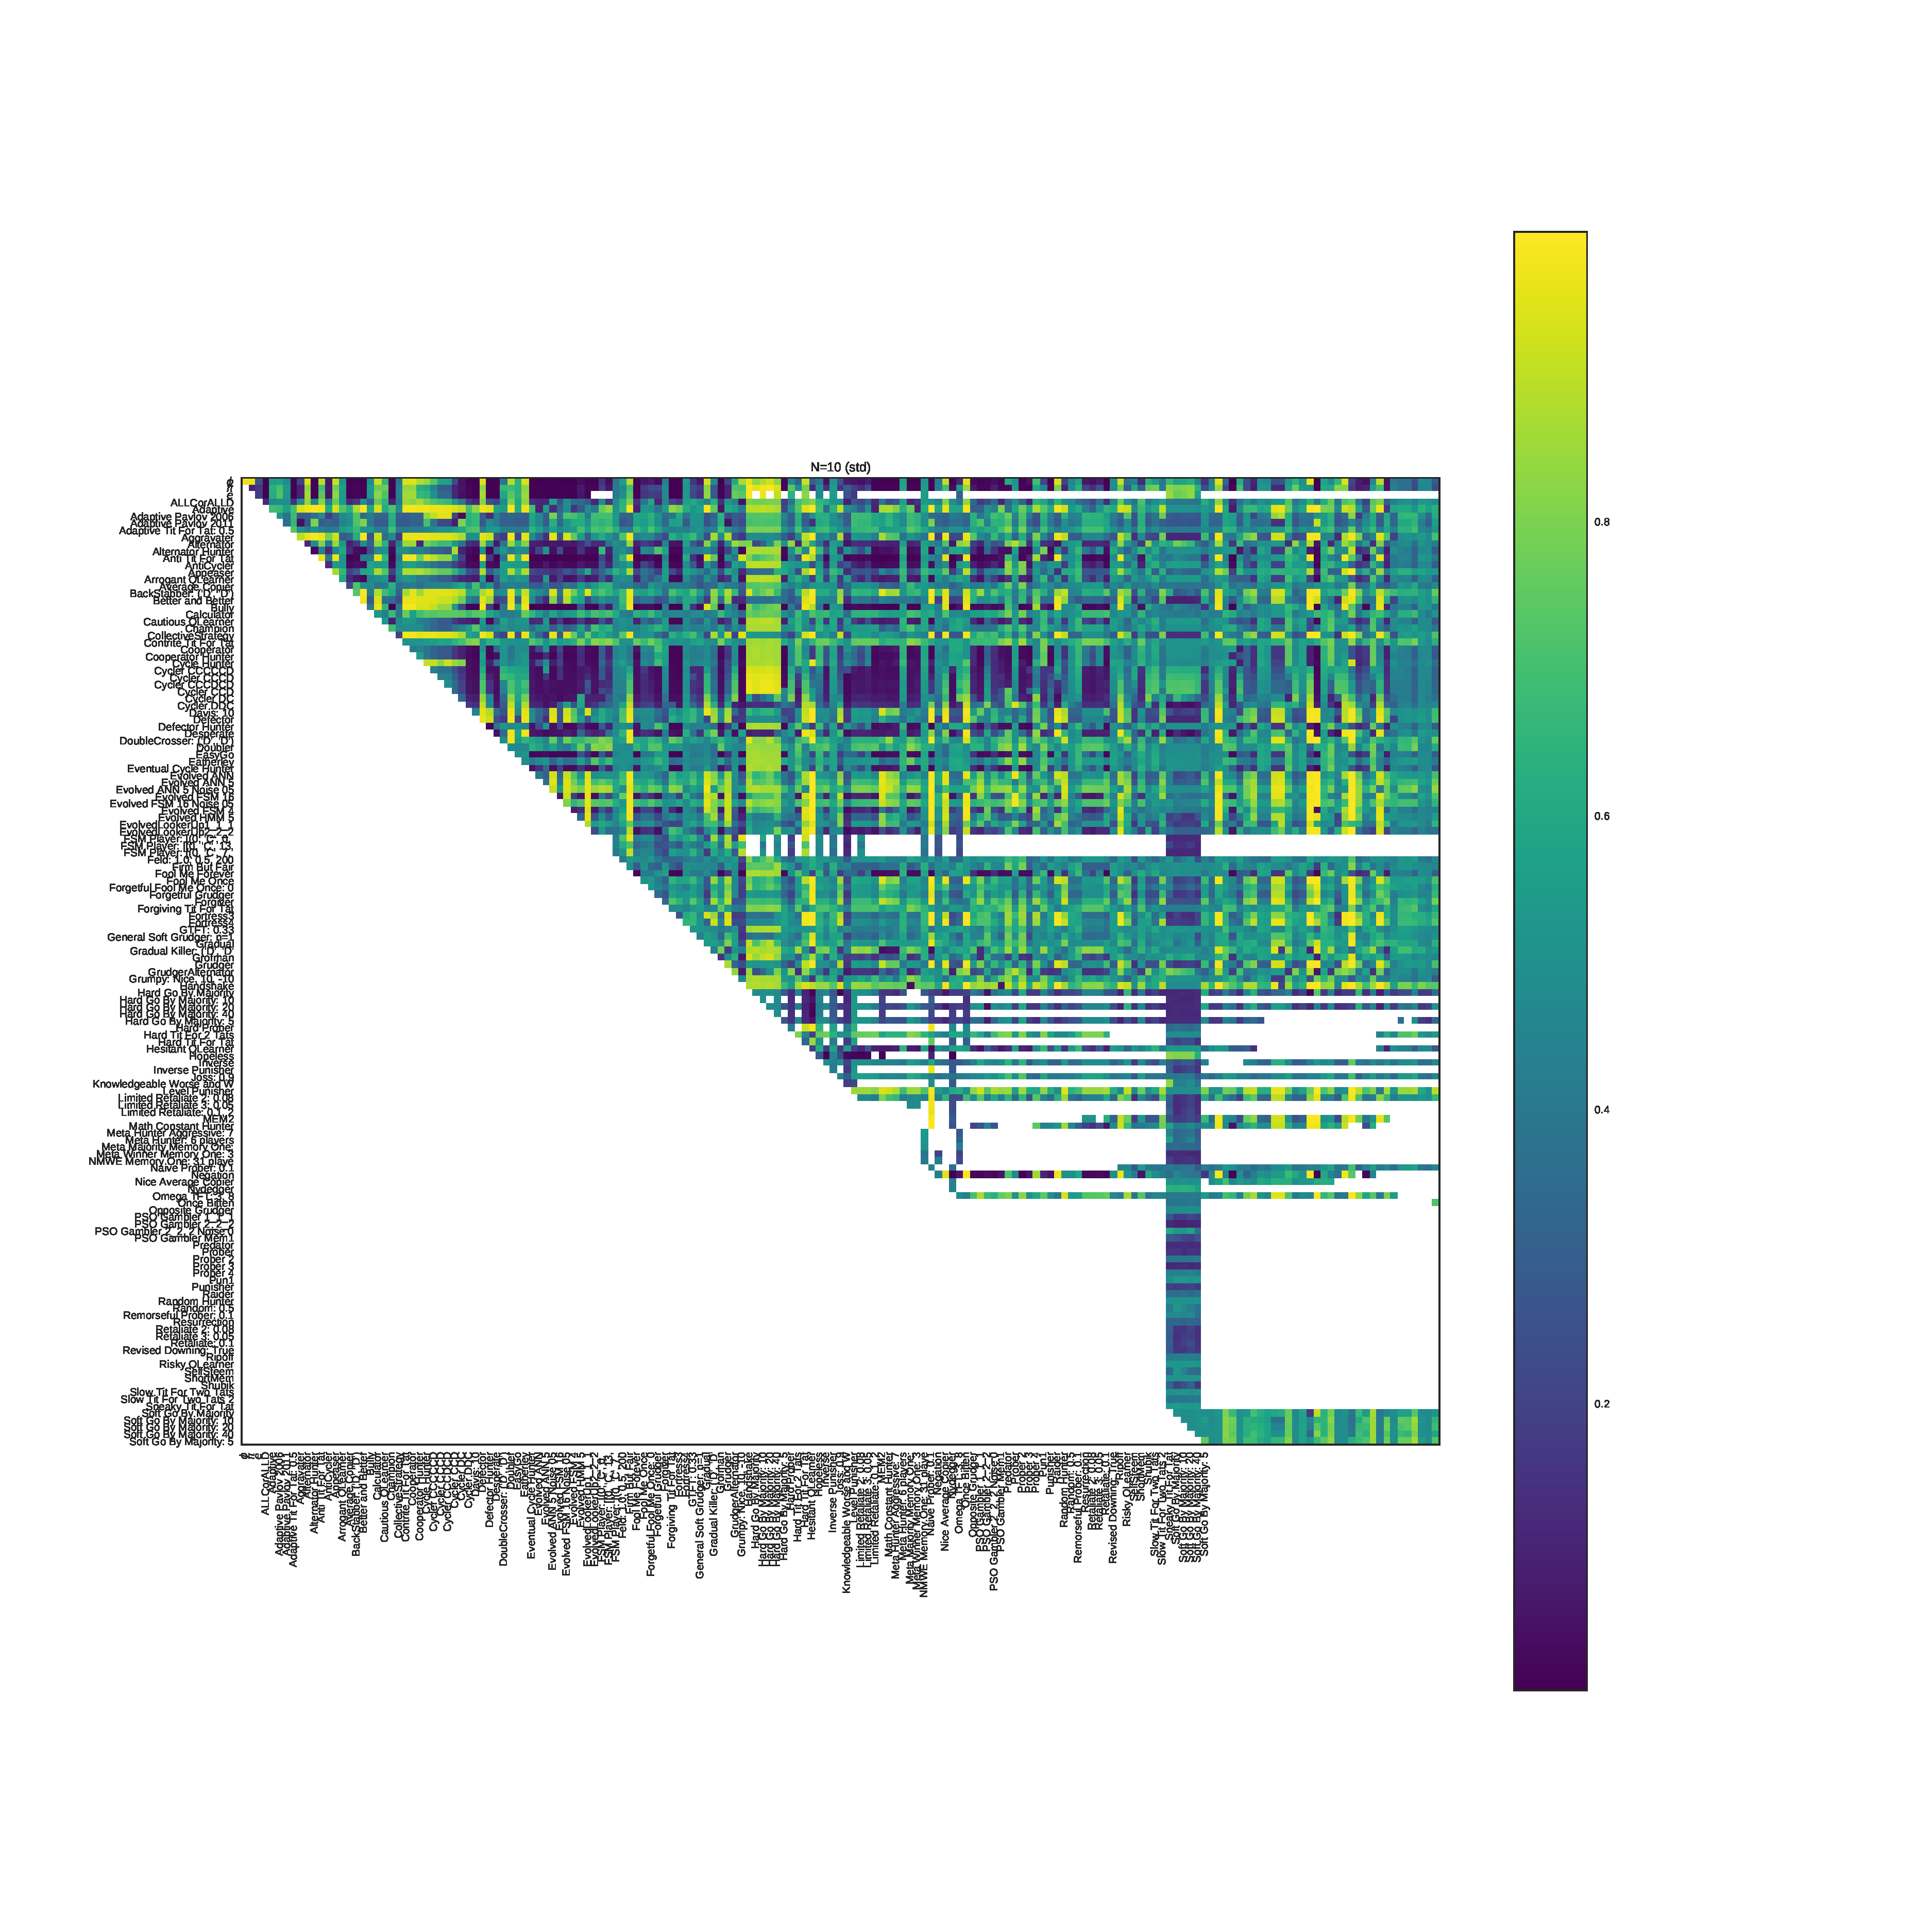
\includegraphics[width=.8\textwidth]{../img/fixation_heatmap_10_std.pdf}
        \caption{\(N=10\)}
    \end{subfigure}%
    ~
    \begin{subfigure}[t]{.3\textwidth}
        \centering
        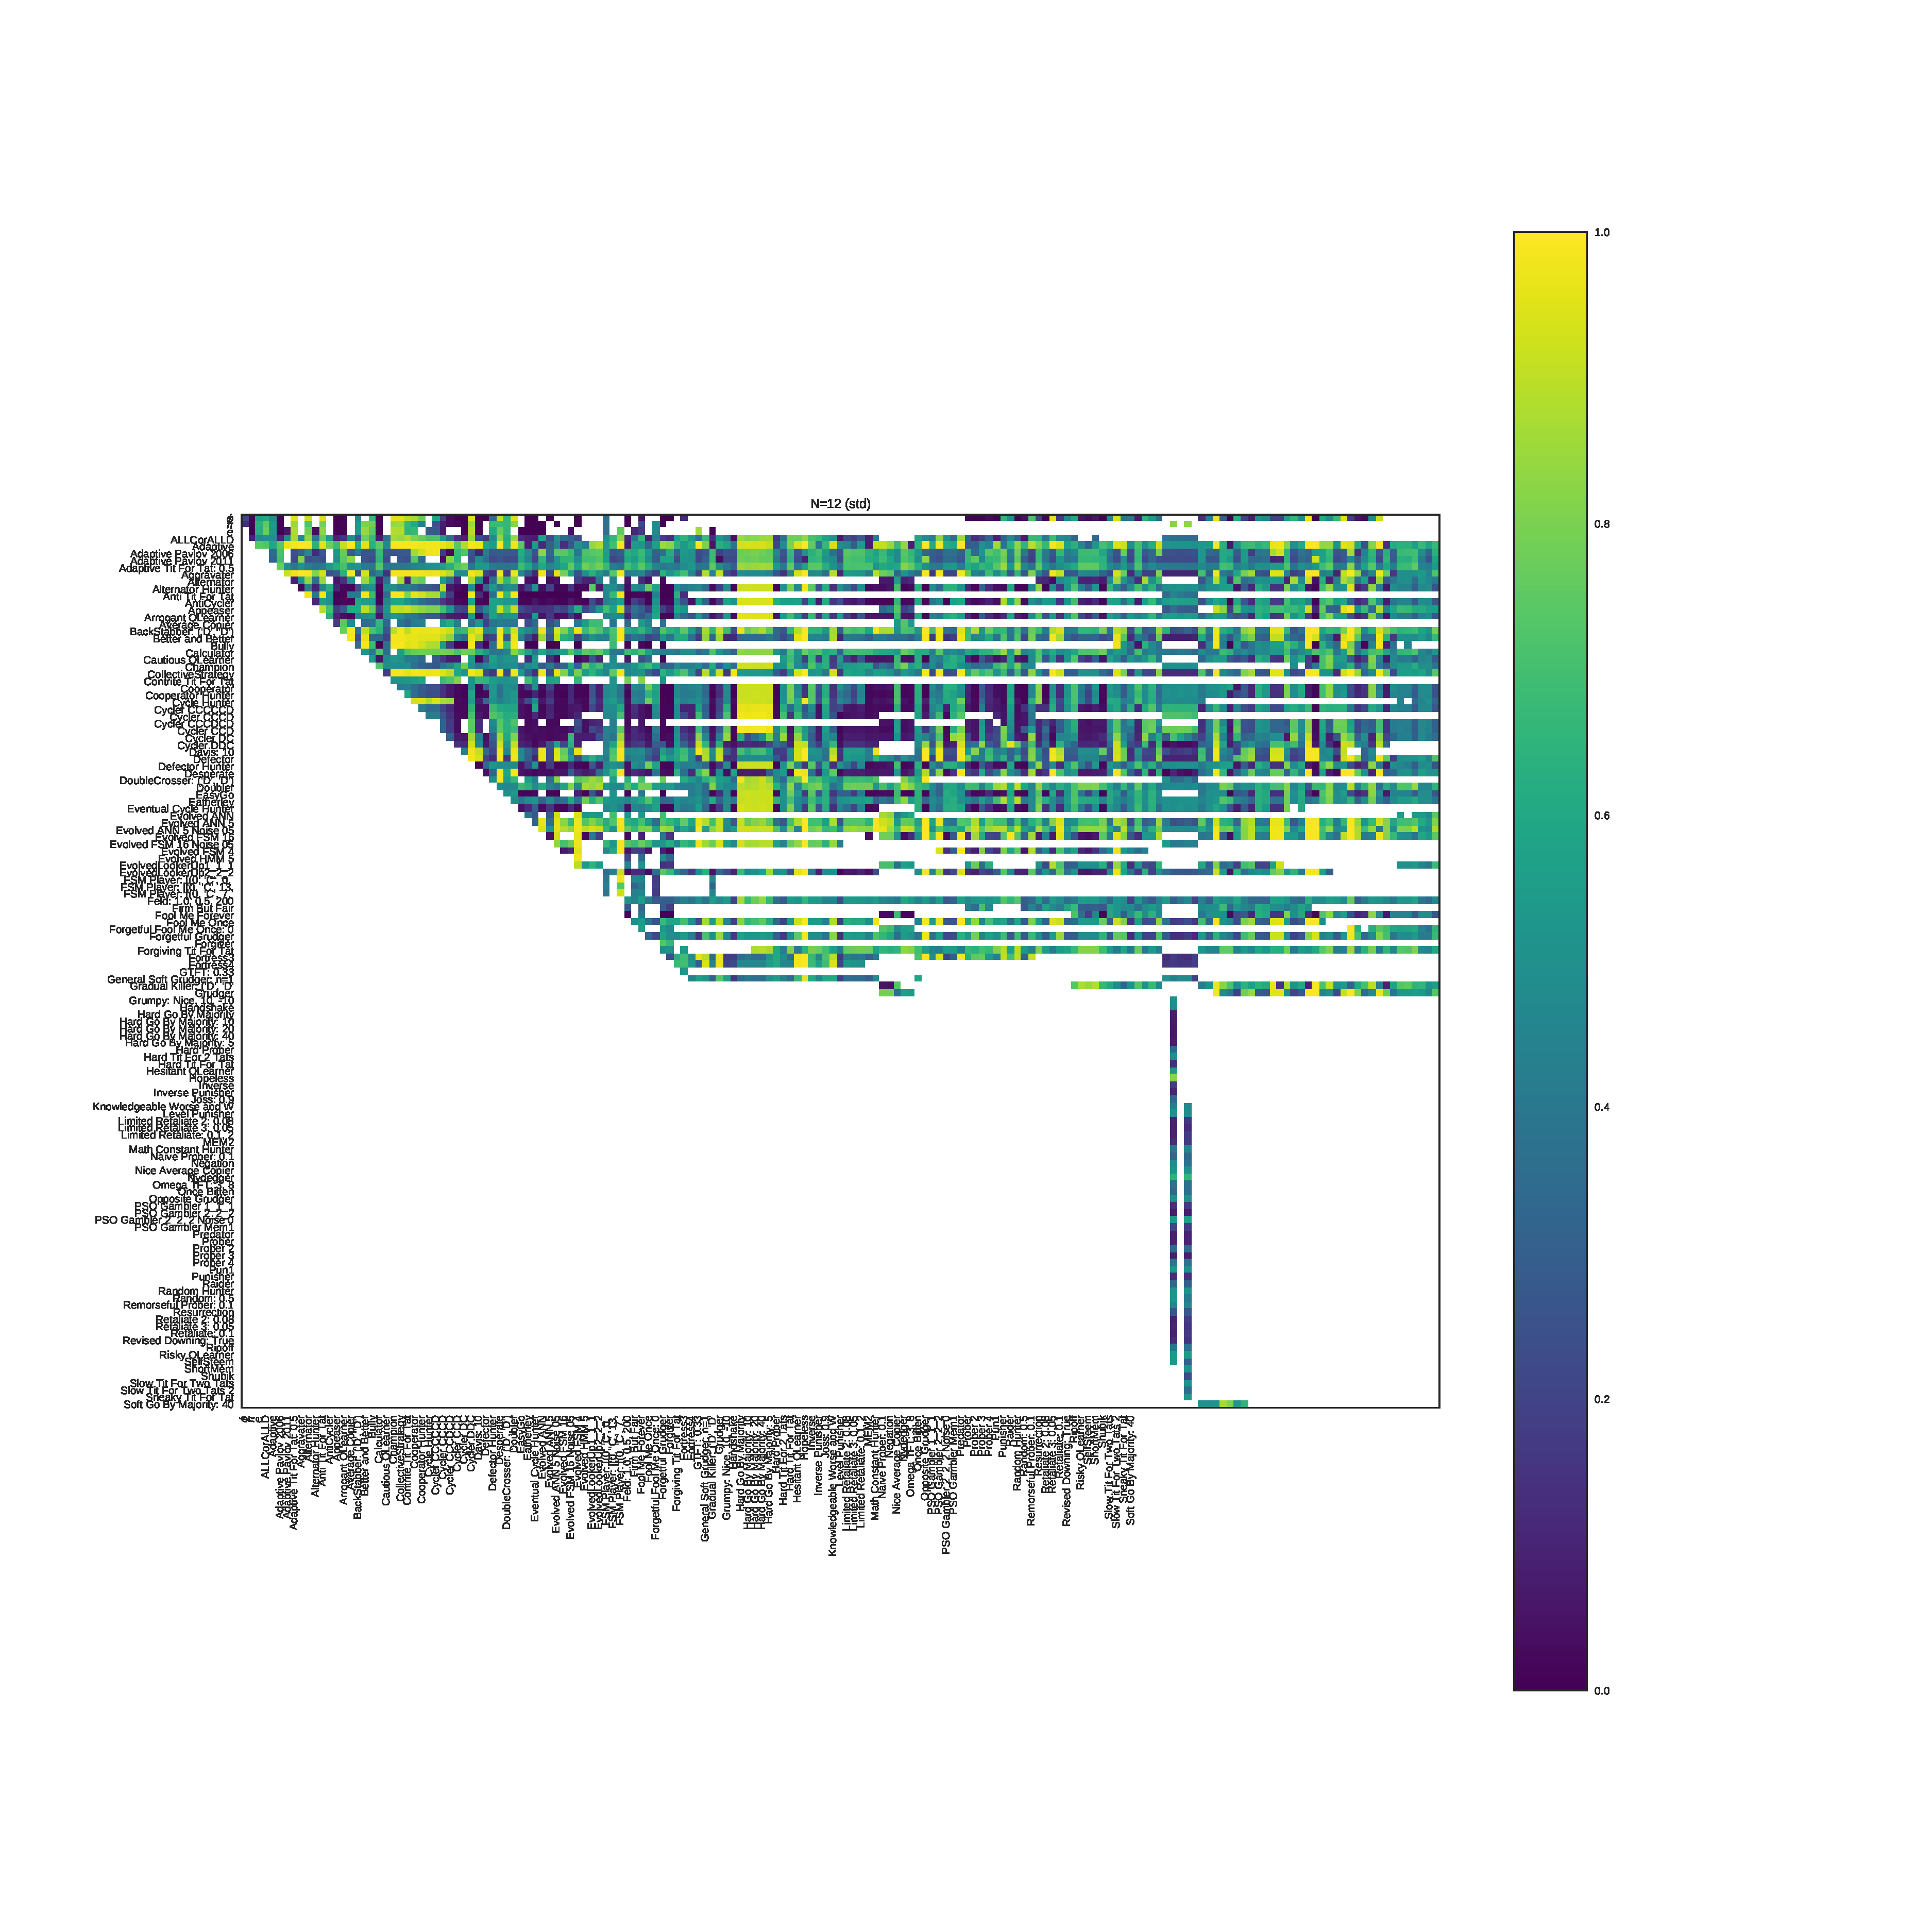
\includegraphics[width=.8\textwidth]{../img/fixation_heatmap_12_std.pdf}
        \caption{\(N=12\)}
    \end{subfigure}%

    \begin{subfigure}[t]{.3\textwidth}
        \centering
        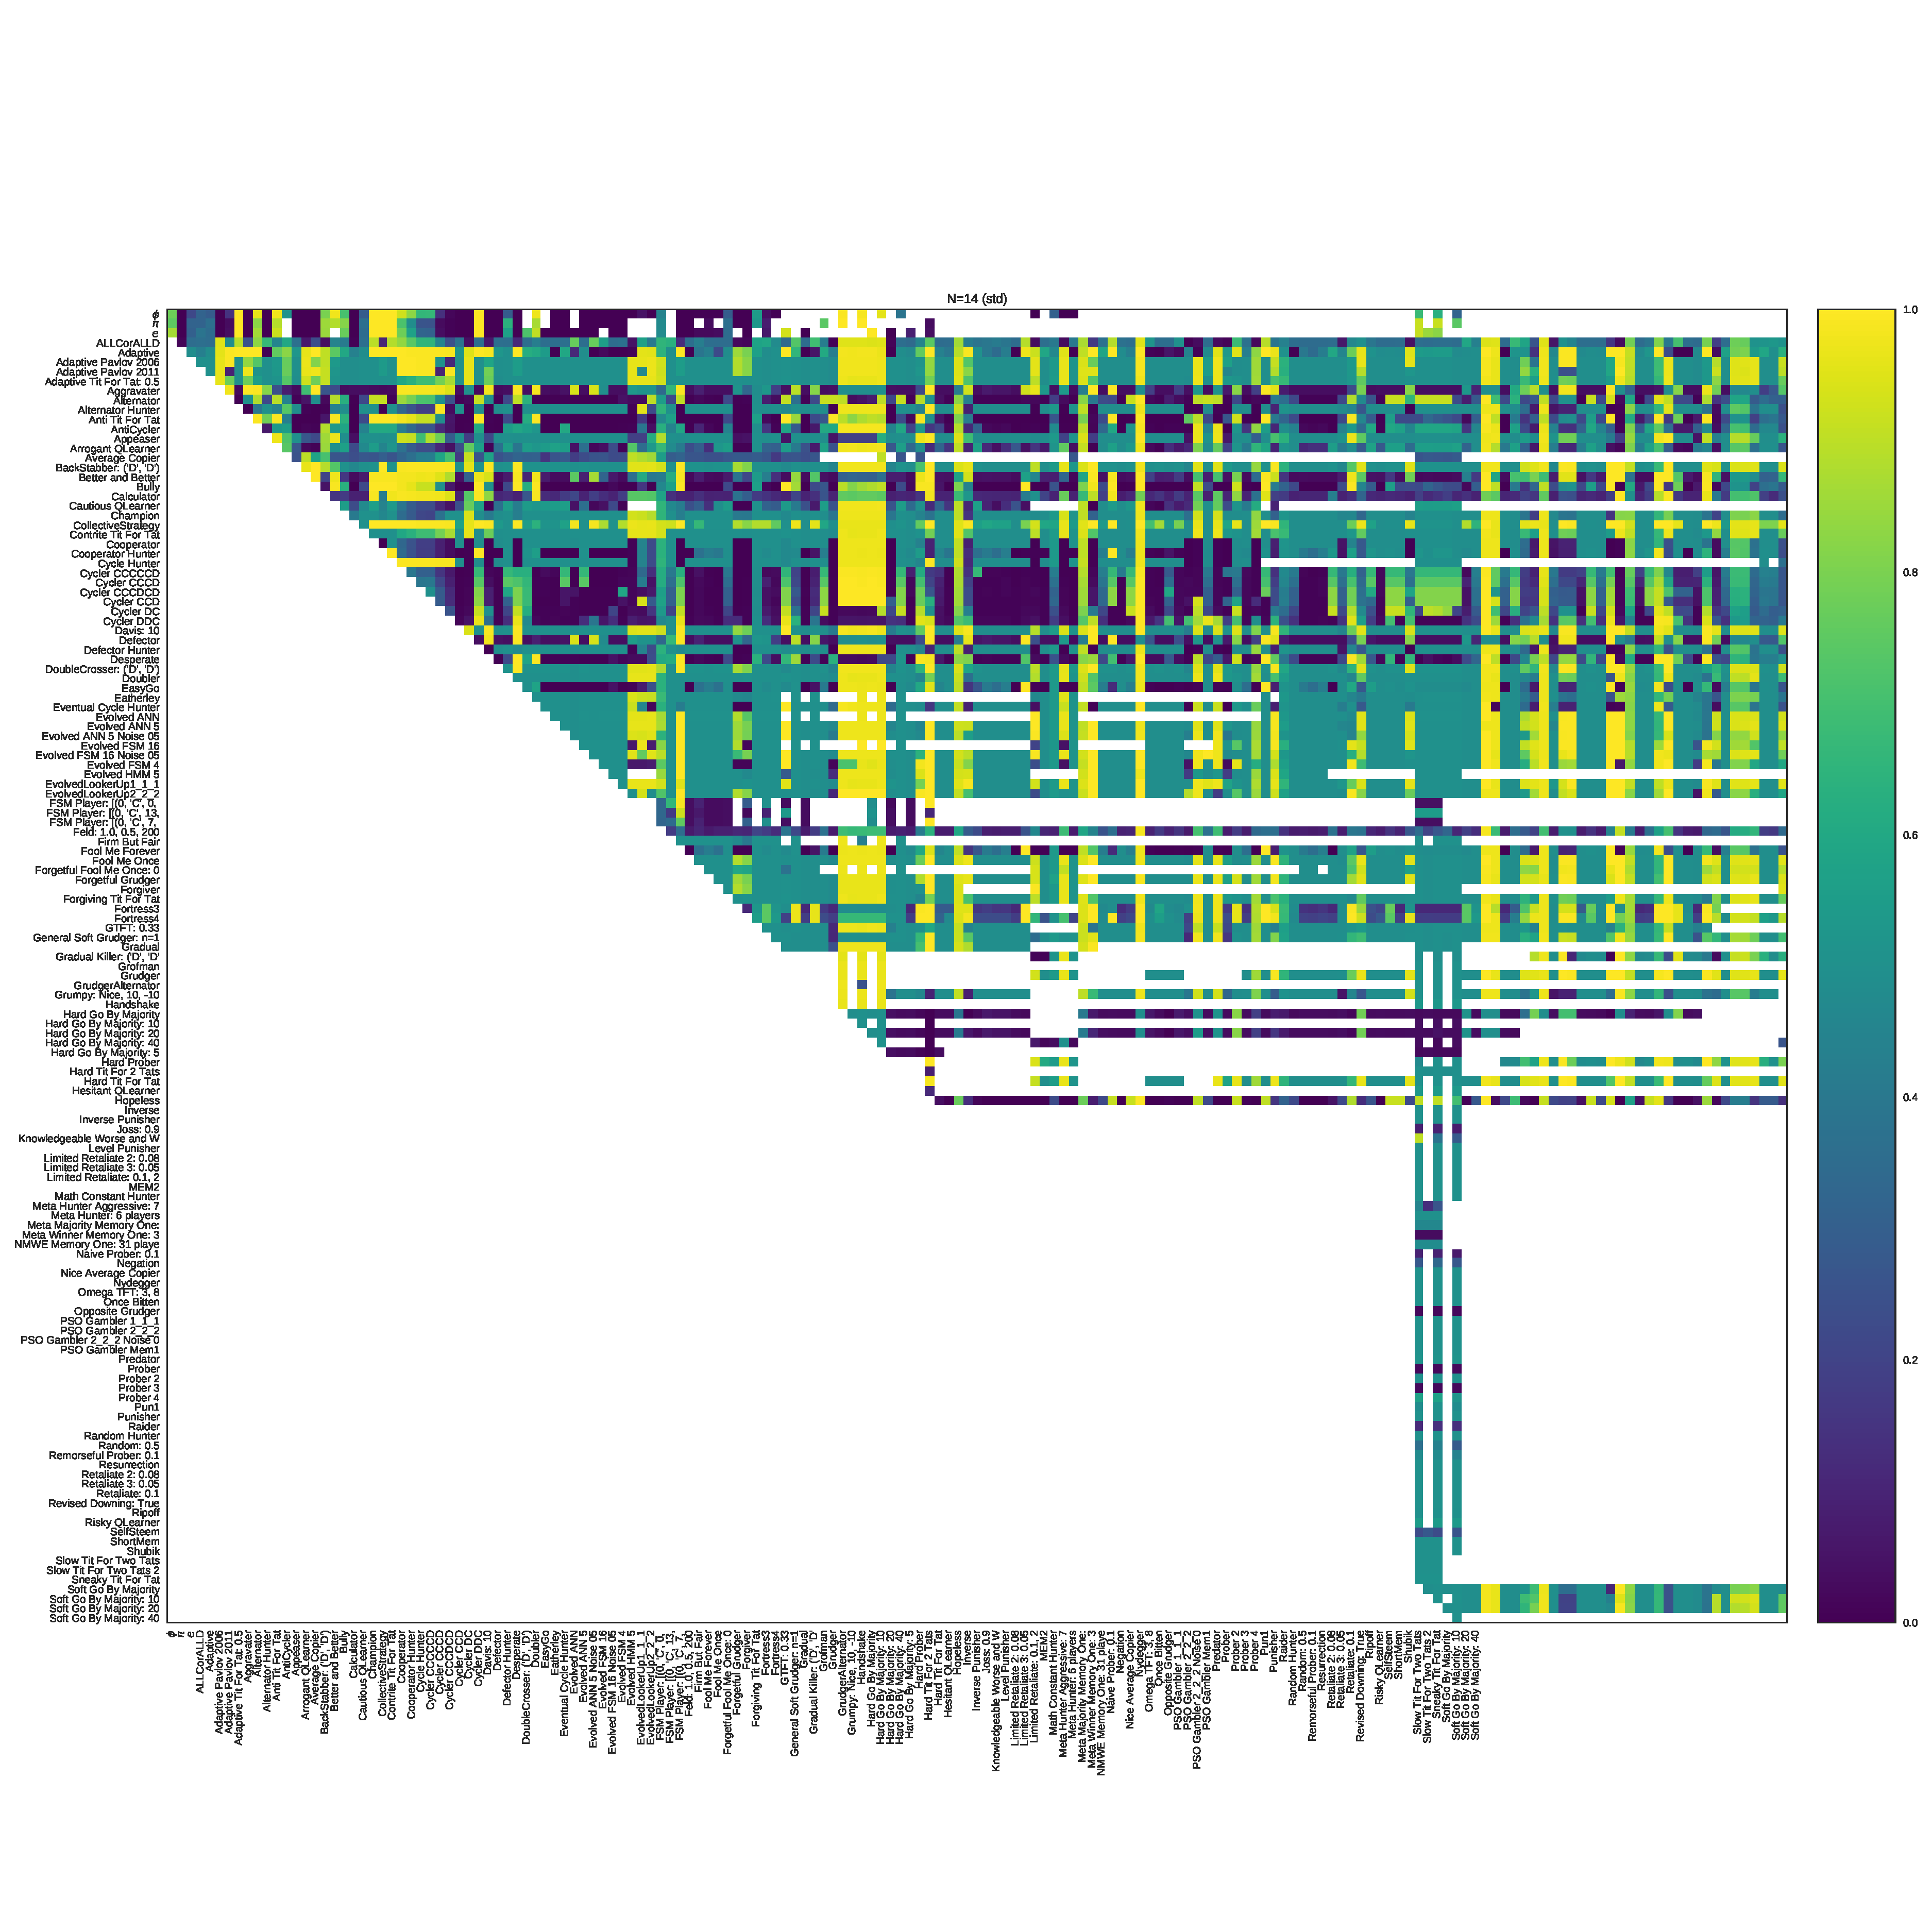
\includegraphics[width=.8\textwidth]{../img/fixation_heatmap_14_std.pdf}
        \caption{\(N=14\)}
    \end{subfigure}%
    \caption{Pairwise fixation probabilities of all strategies}
    \label{fig:fixation_heatmap_std}
\end{figure}

\begin{figure}[!hbtp]
    \centering
    \begin{subfigure}[t]{.3\textwidth}
        \centering
        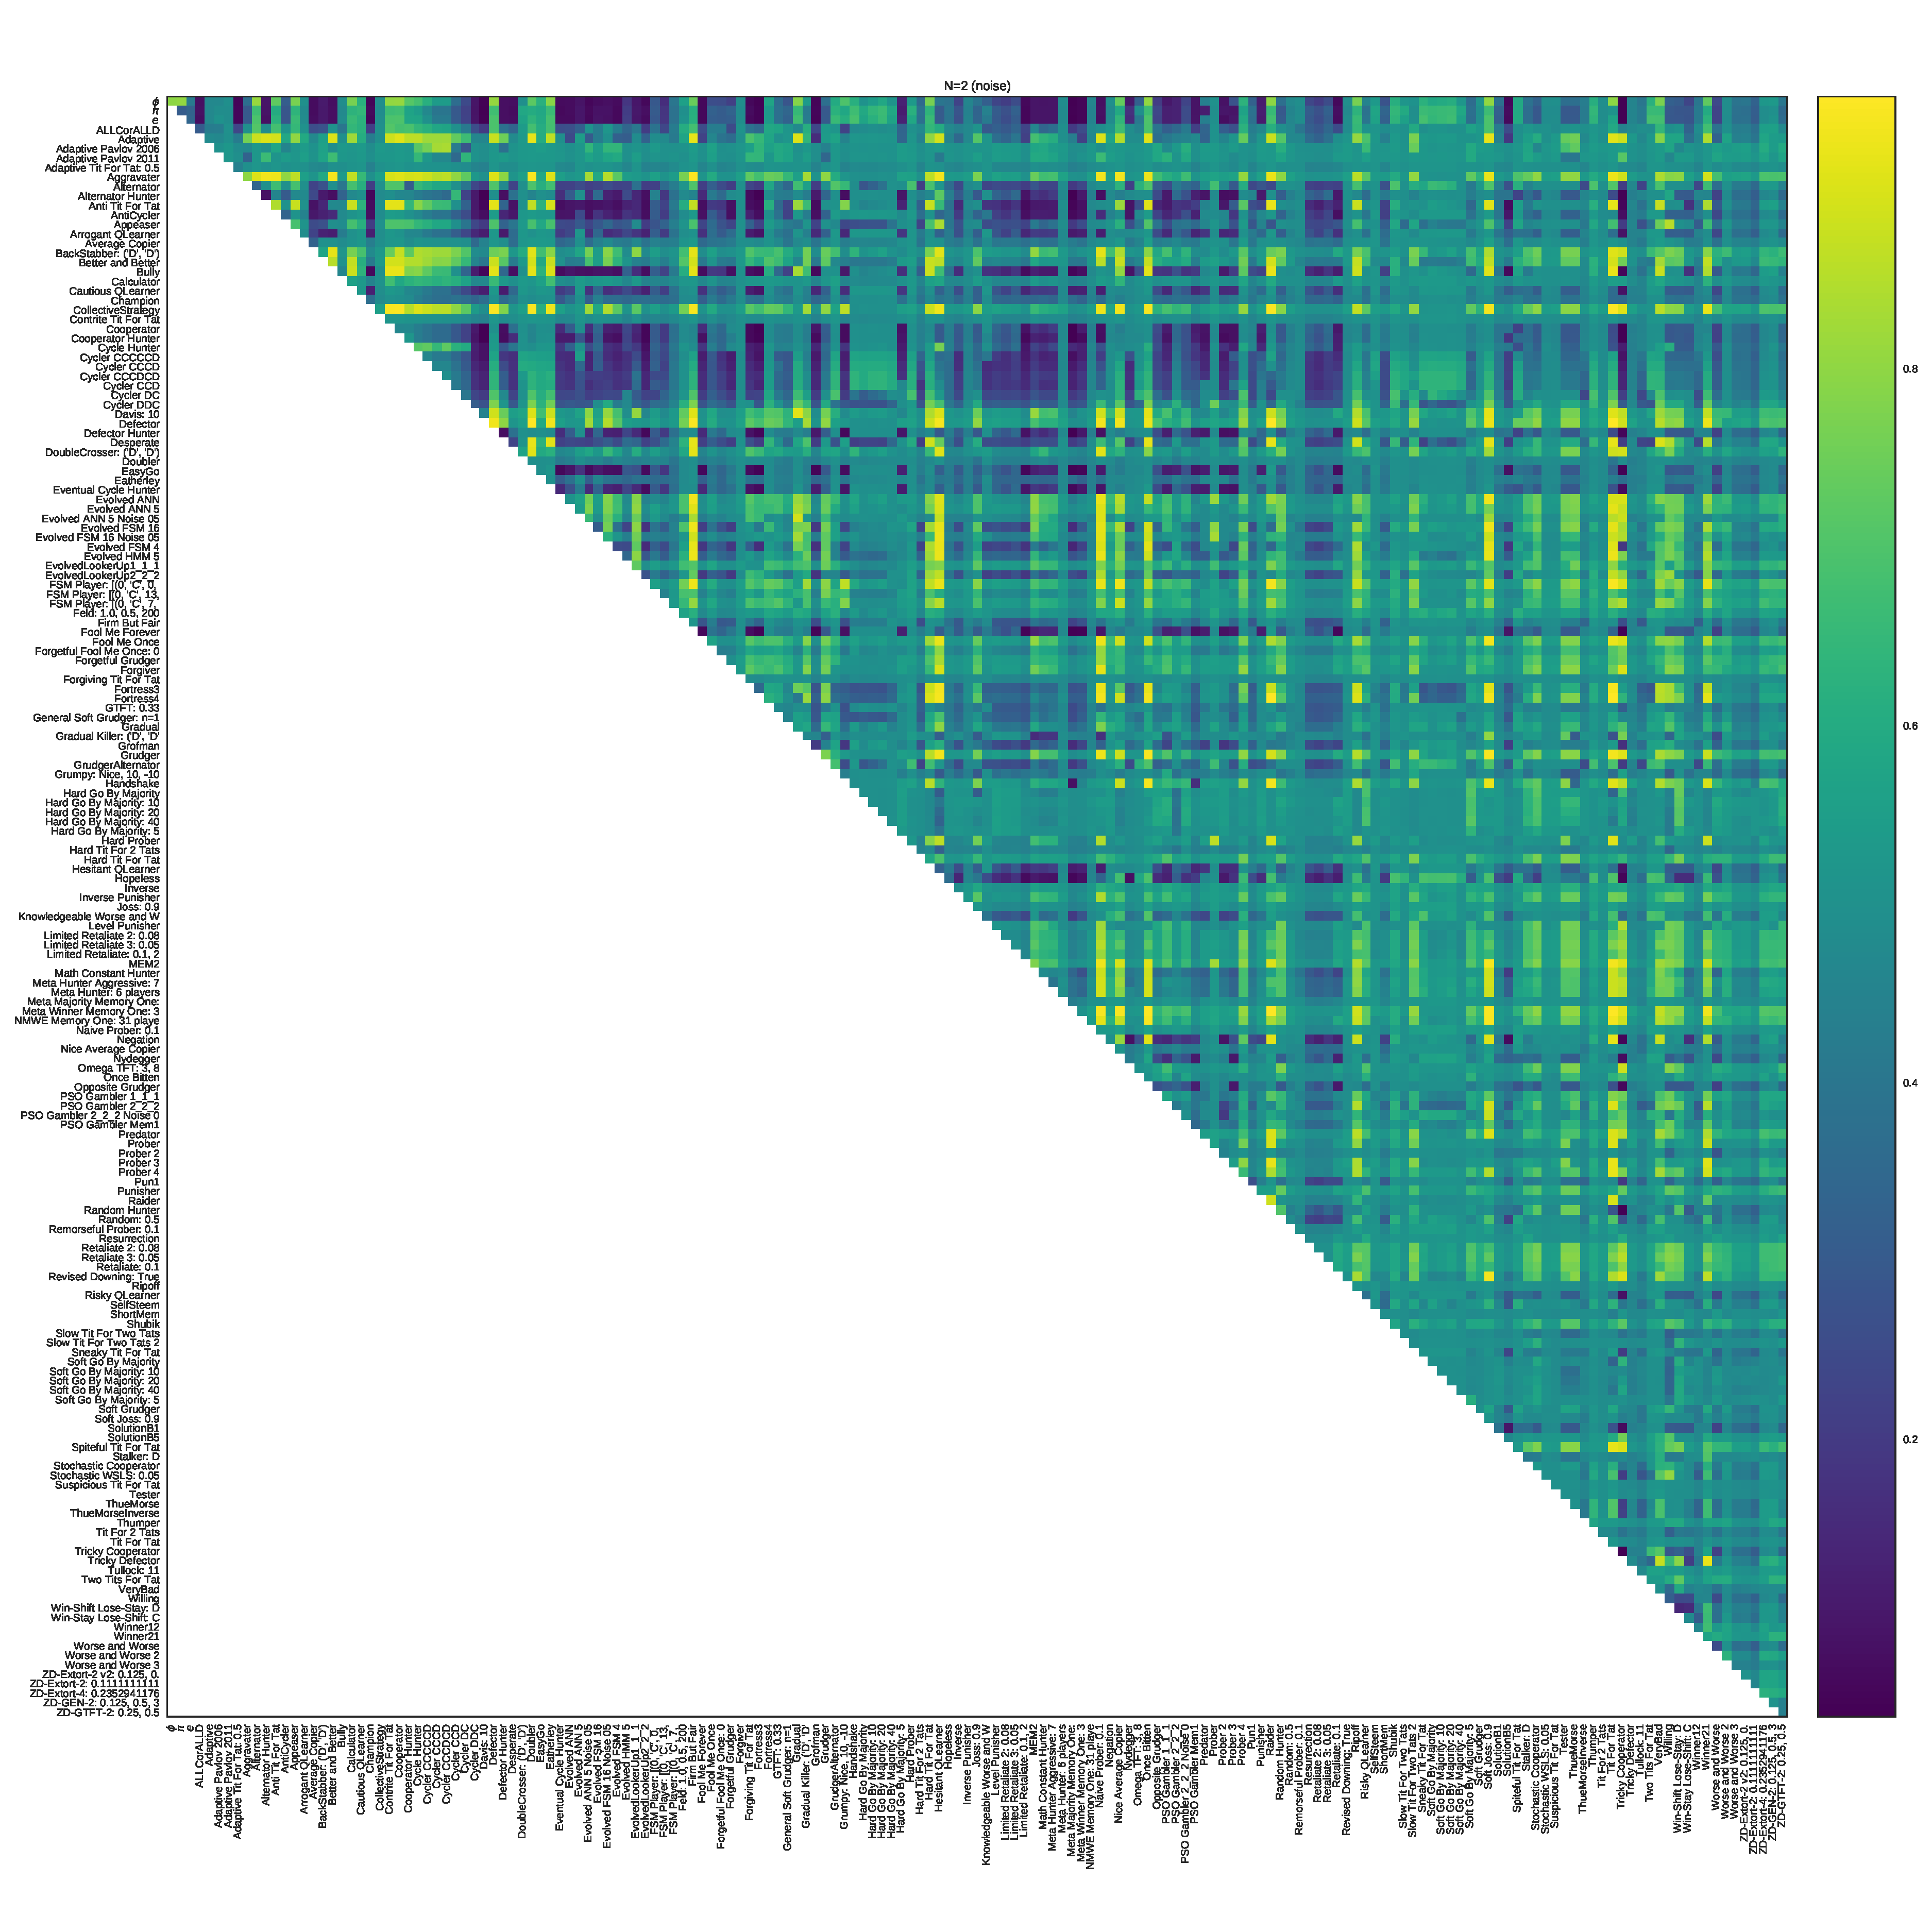
\includegraphics[width=.8\textwidth]{../img/fixation_heatmap_2_noise.pdf}
        \caption{\(N=2\)}
    \end{subfigure}%
    ~
    \begin{subfigure}[t]{.3\textwidth}
        \centering
        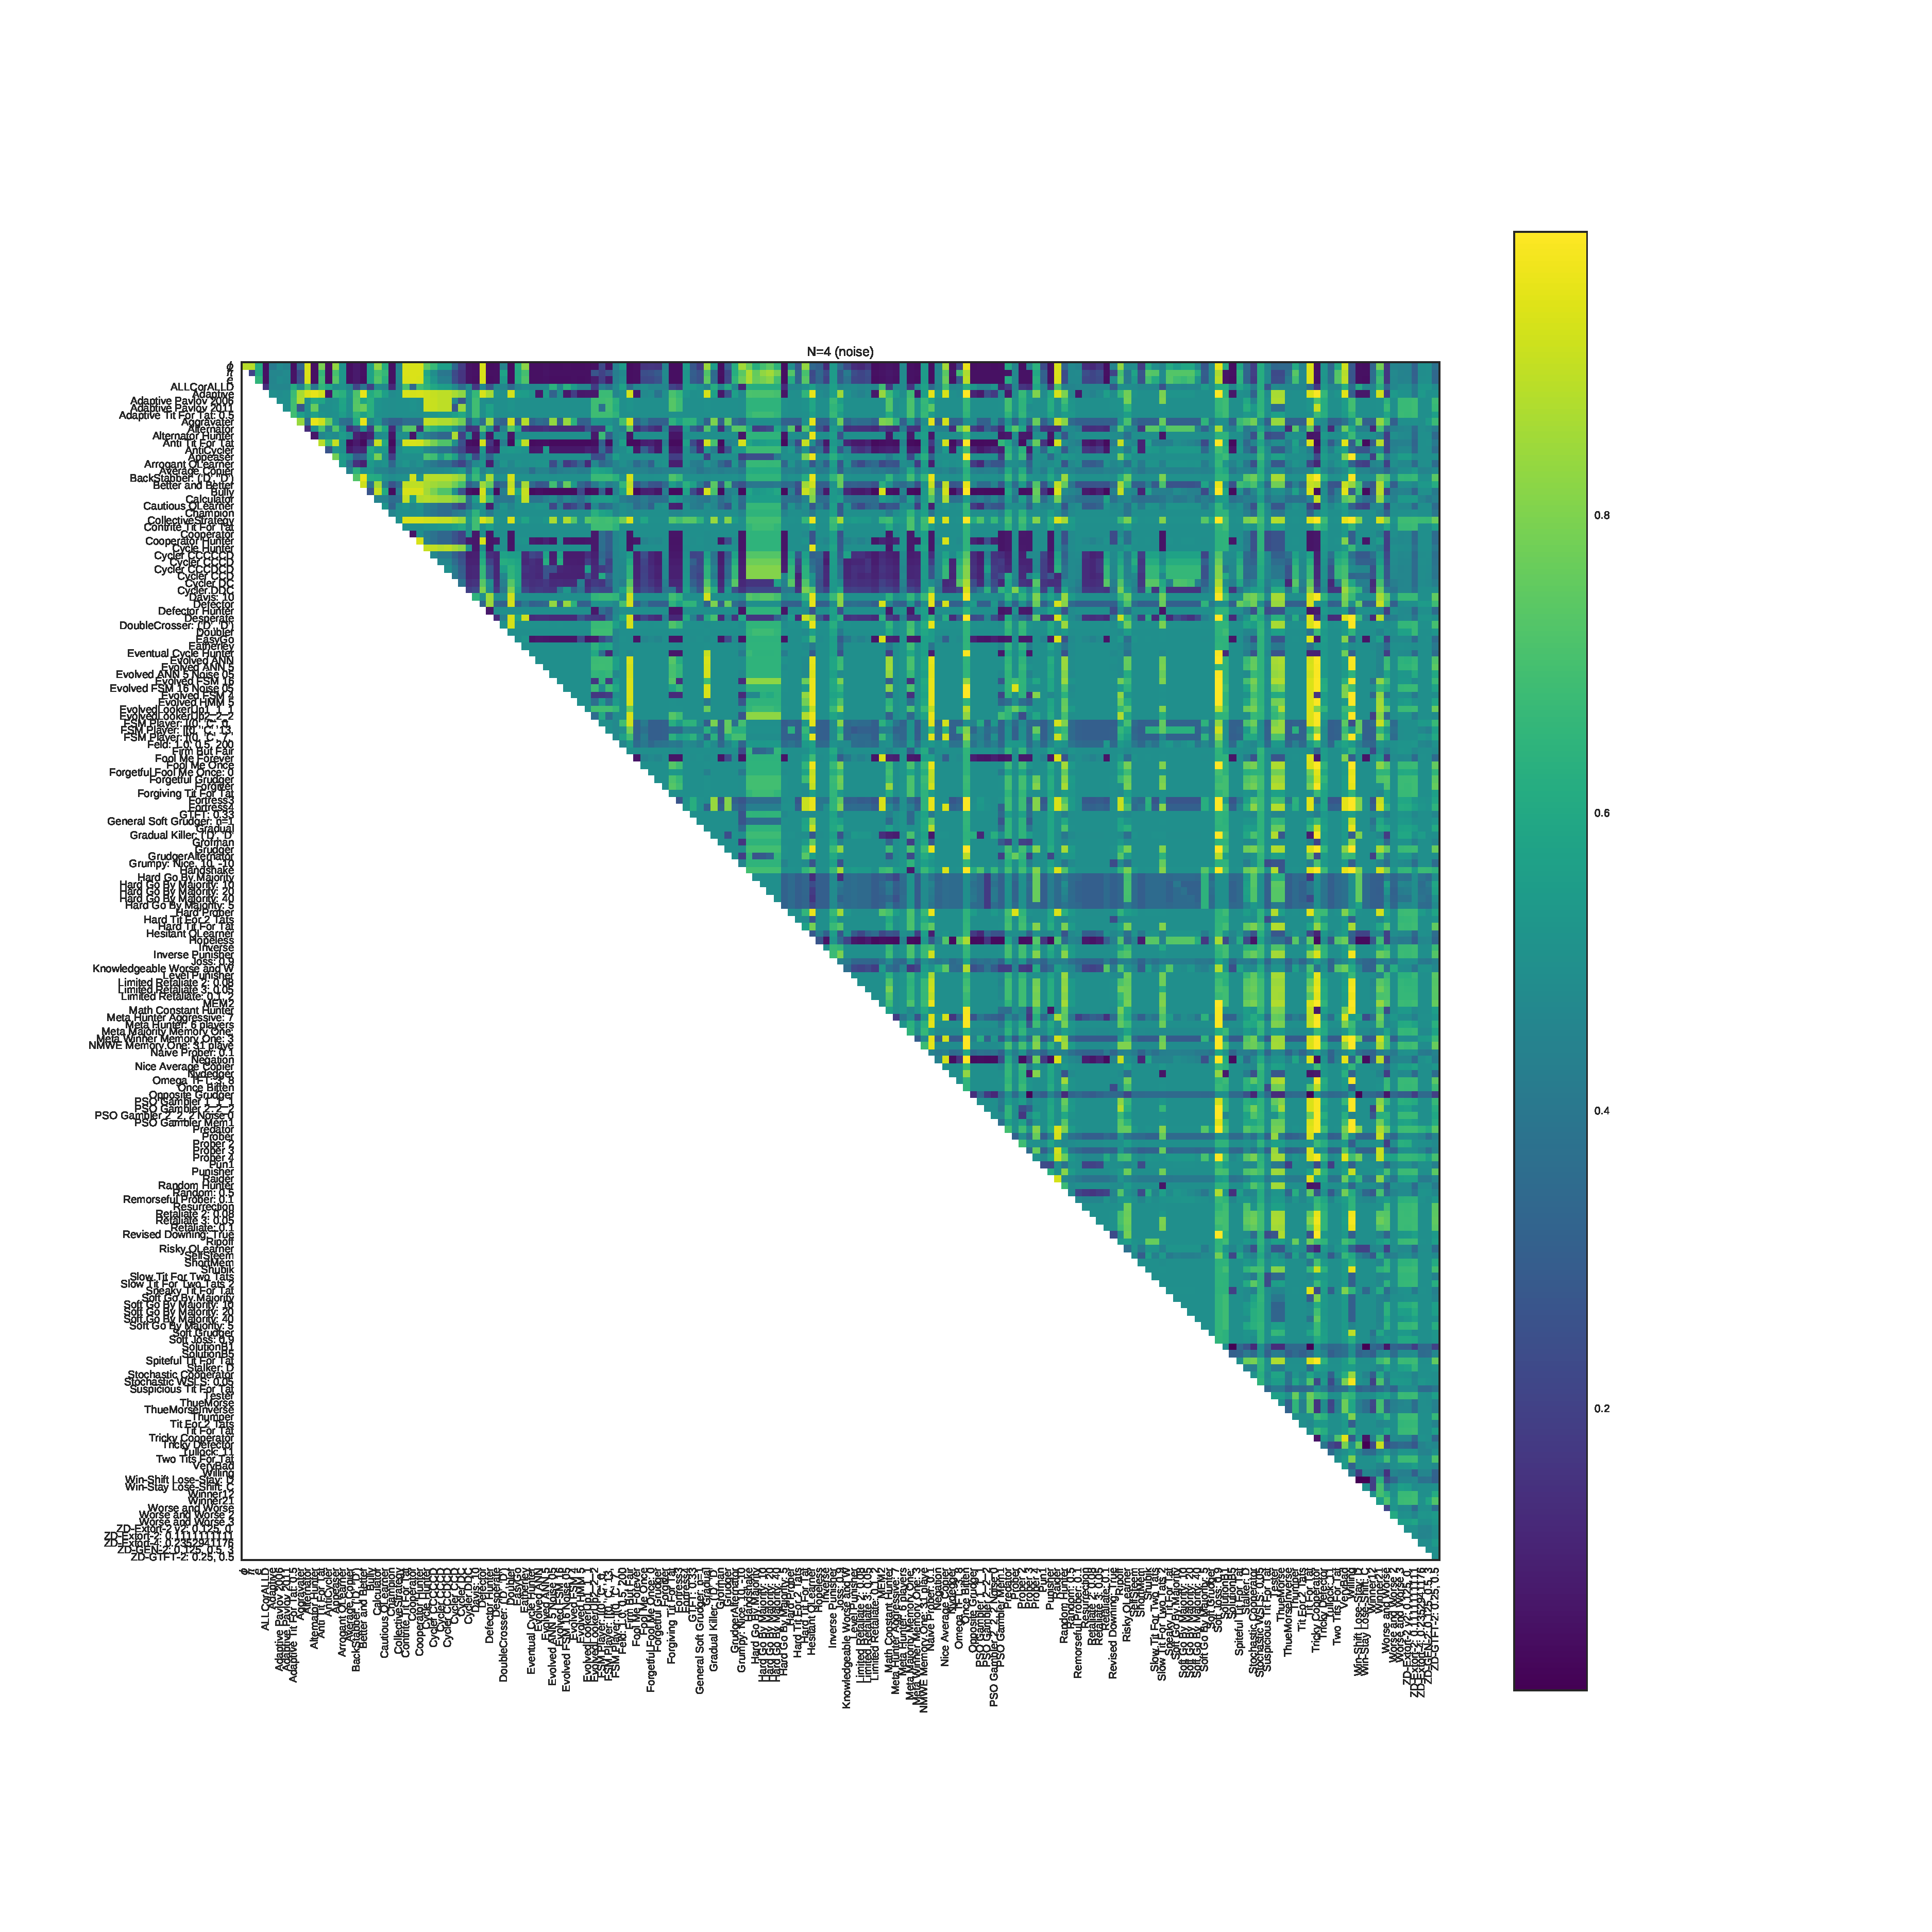
\includegraphics[width=.8\textwidth]{../img/fixation_heatmap_4_noise.pdf}
        \caption{\(N=4\)}
    \end{subfigure}%
    ~
    \begin{subfigure}[t]{.3\textwidth}
        \centering
        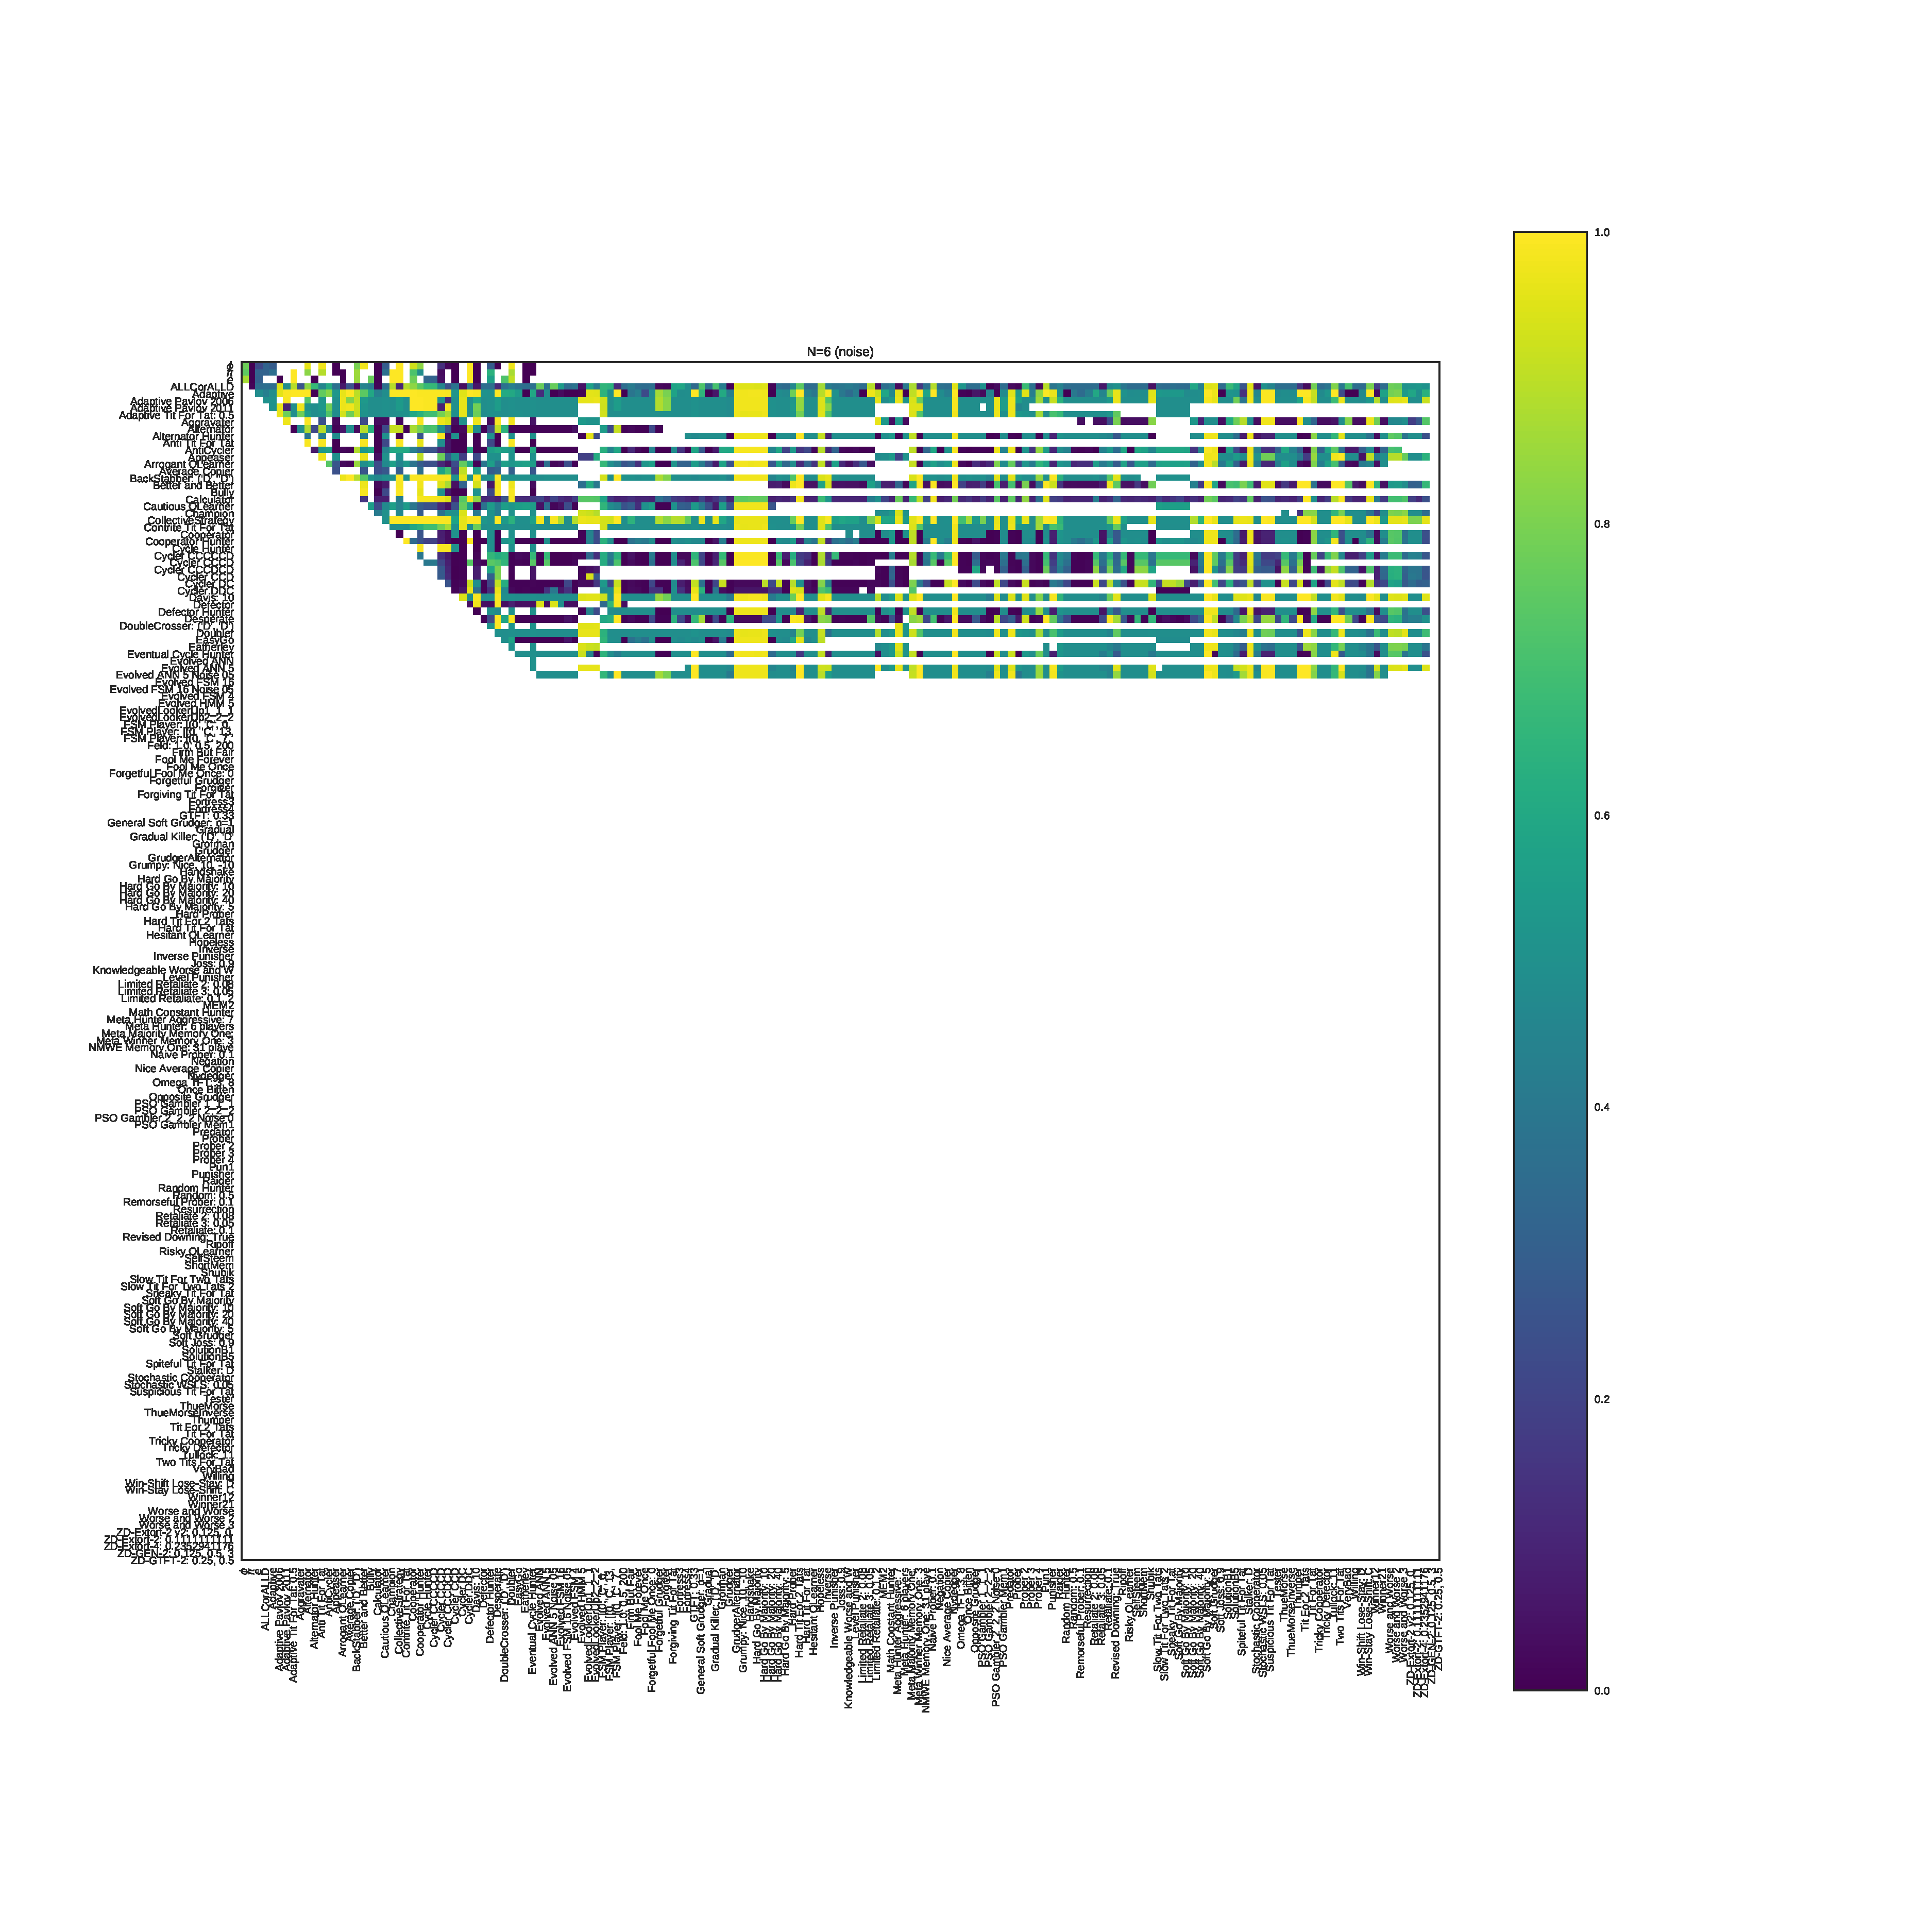
\includegraphics[width=.8\textwidth]{../img/fixation_heatmap_6_noise.pdf}
        \caption{\(N=6\)}
    \end{subfigure}%

    \begin{subfigure}[t]{.3\textwidth}
        \centering
        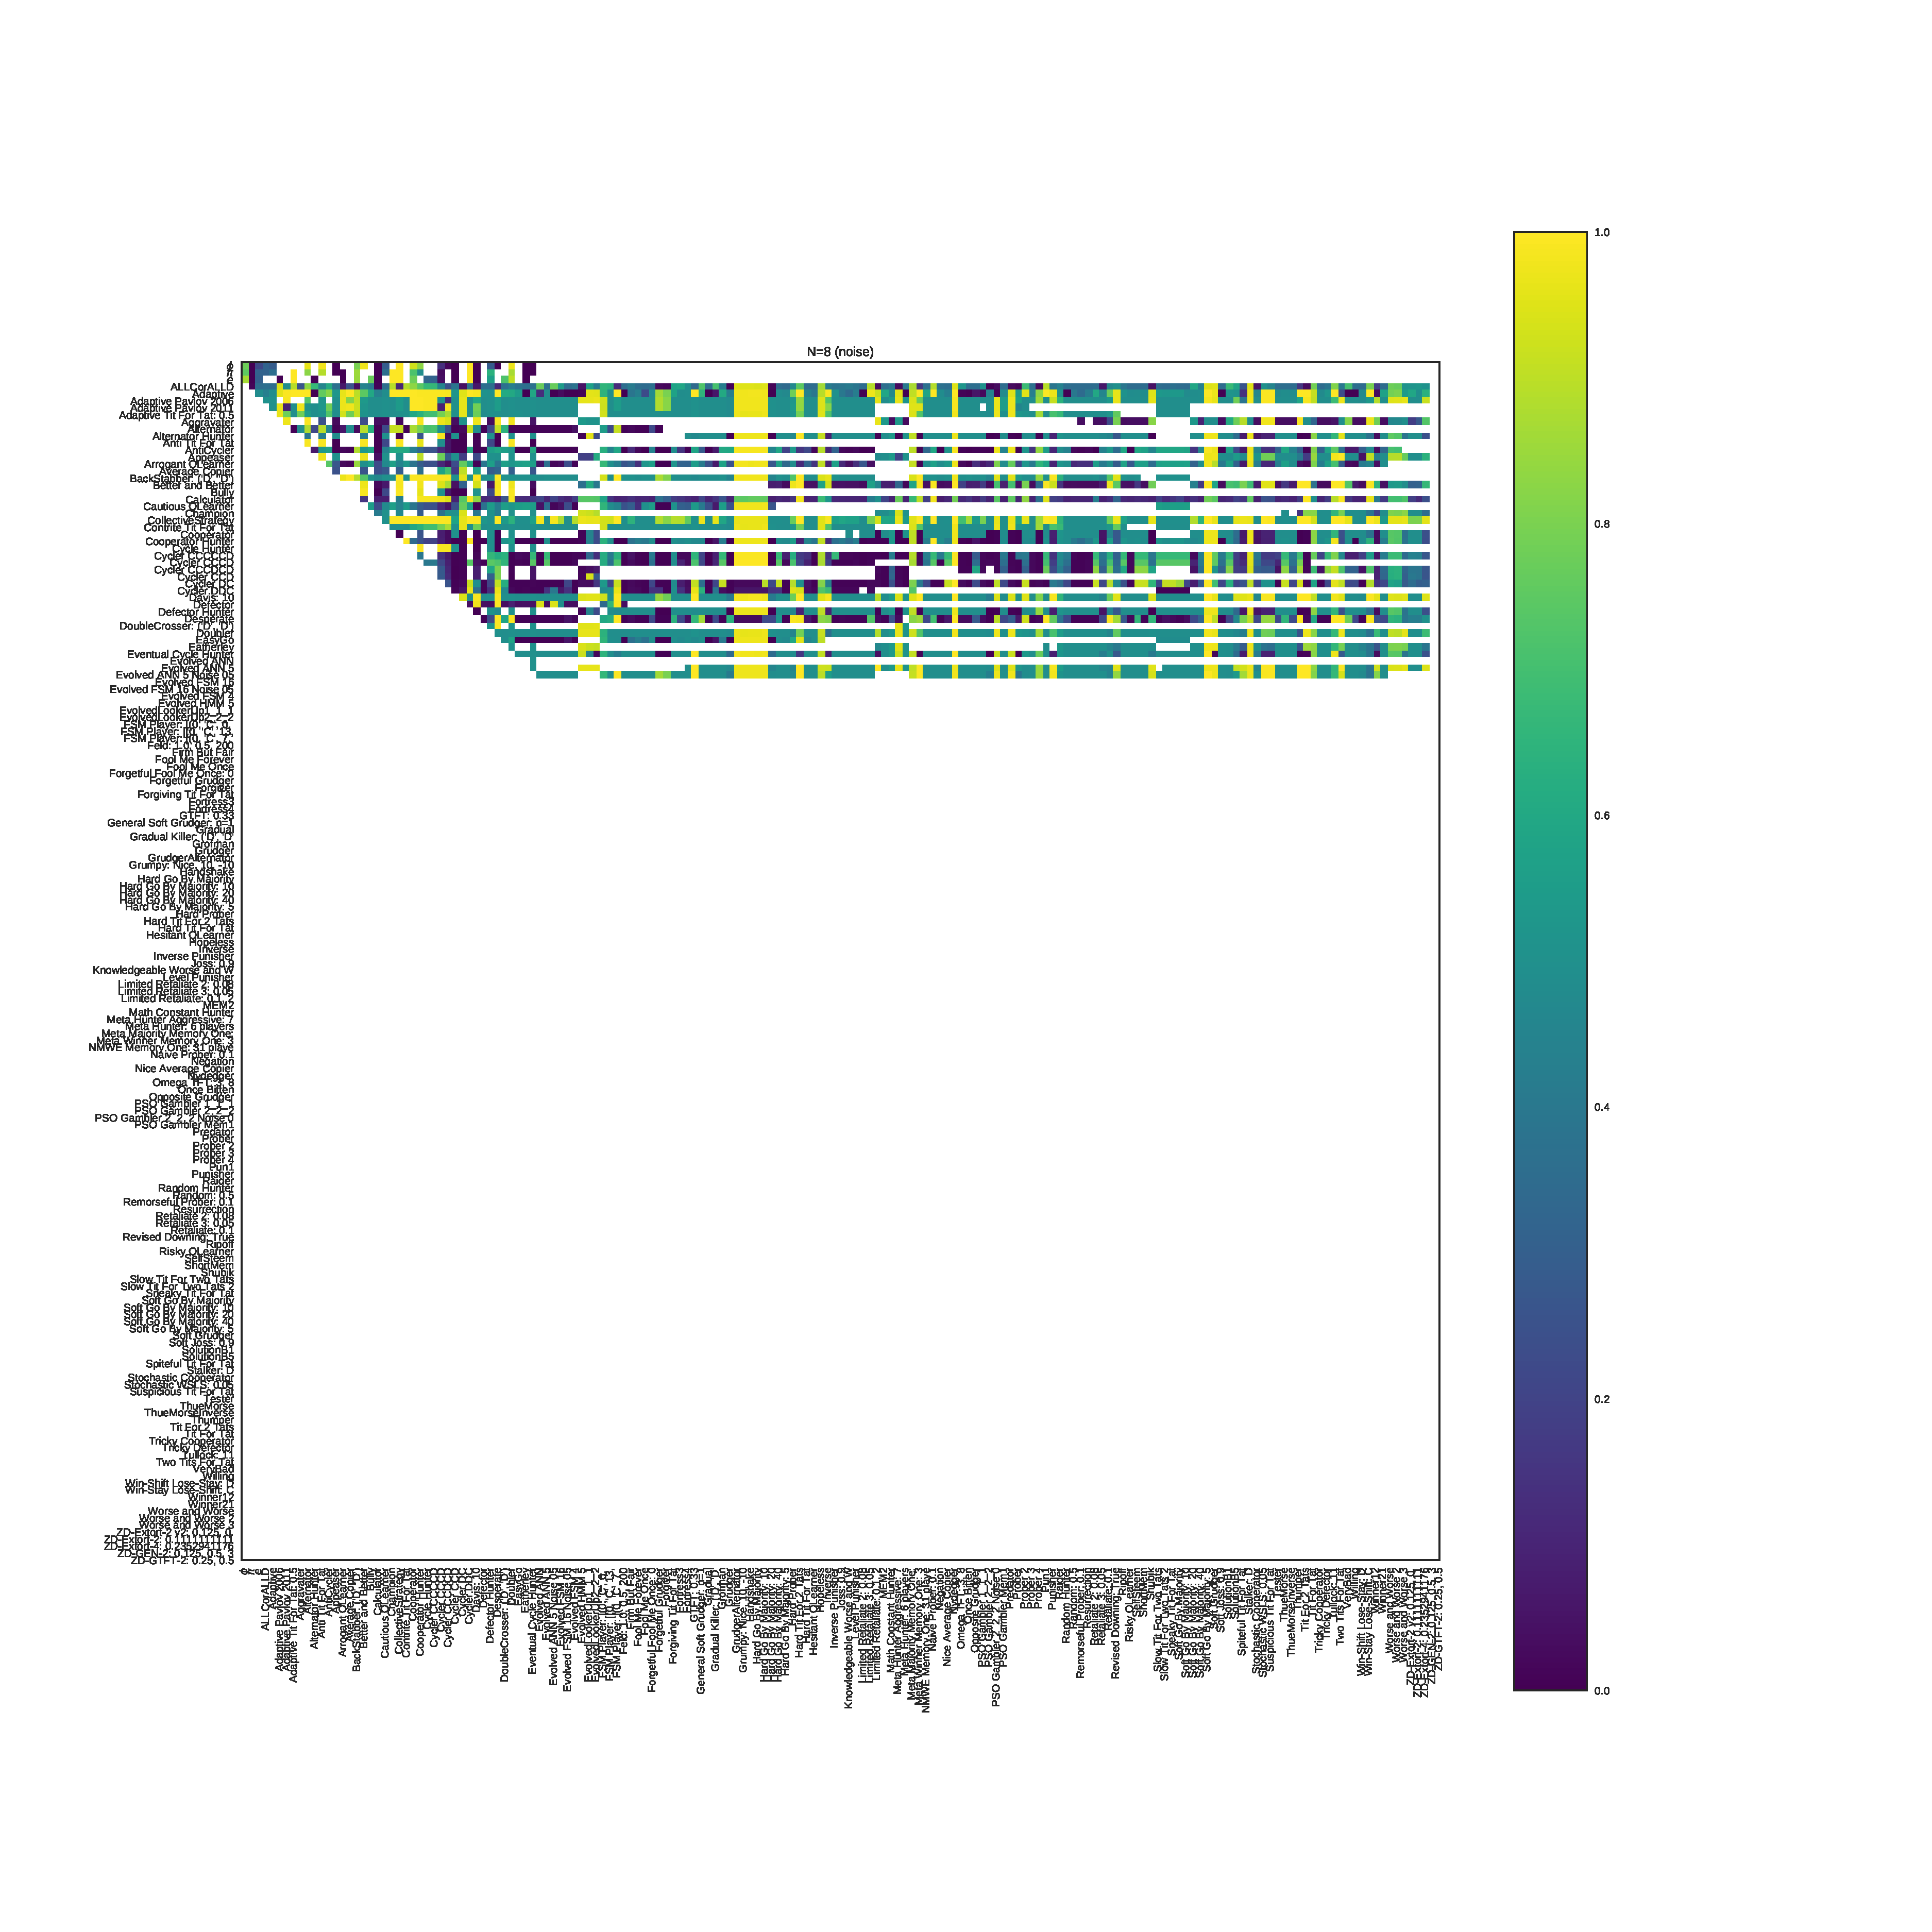
\includegraphics[width=.8\textwidth]{../img/fixation_heatmap_8_noise.pdf}
        \caption{\(N=8\)}
    \end{subfigure}%
    ~
    \begin{subfigure}[t]{.3\textwidth}
        \centering
        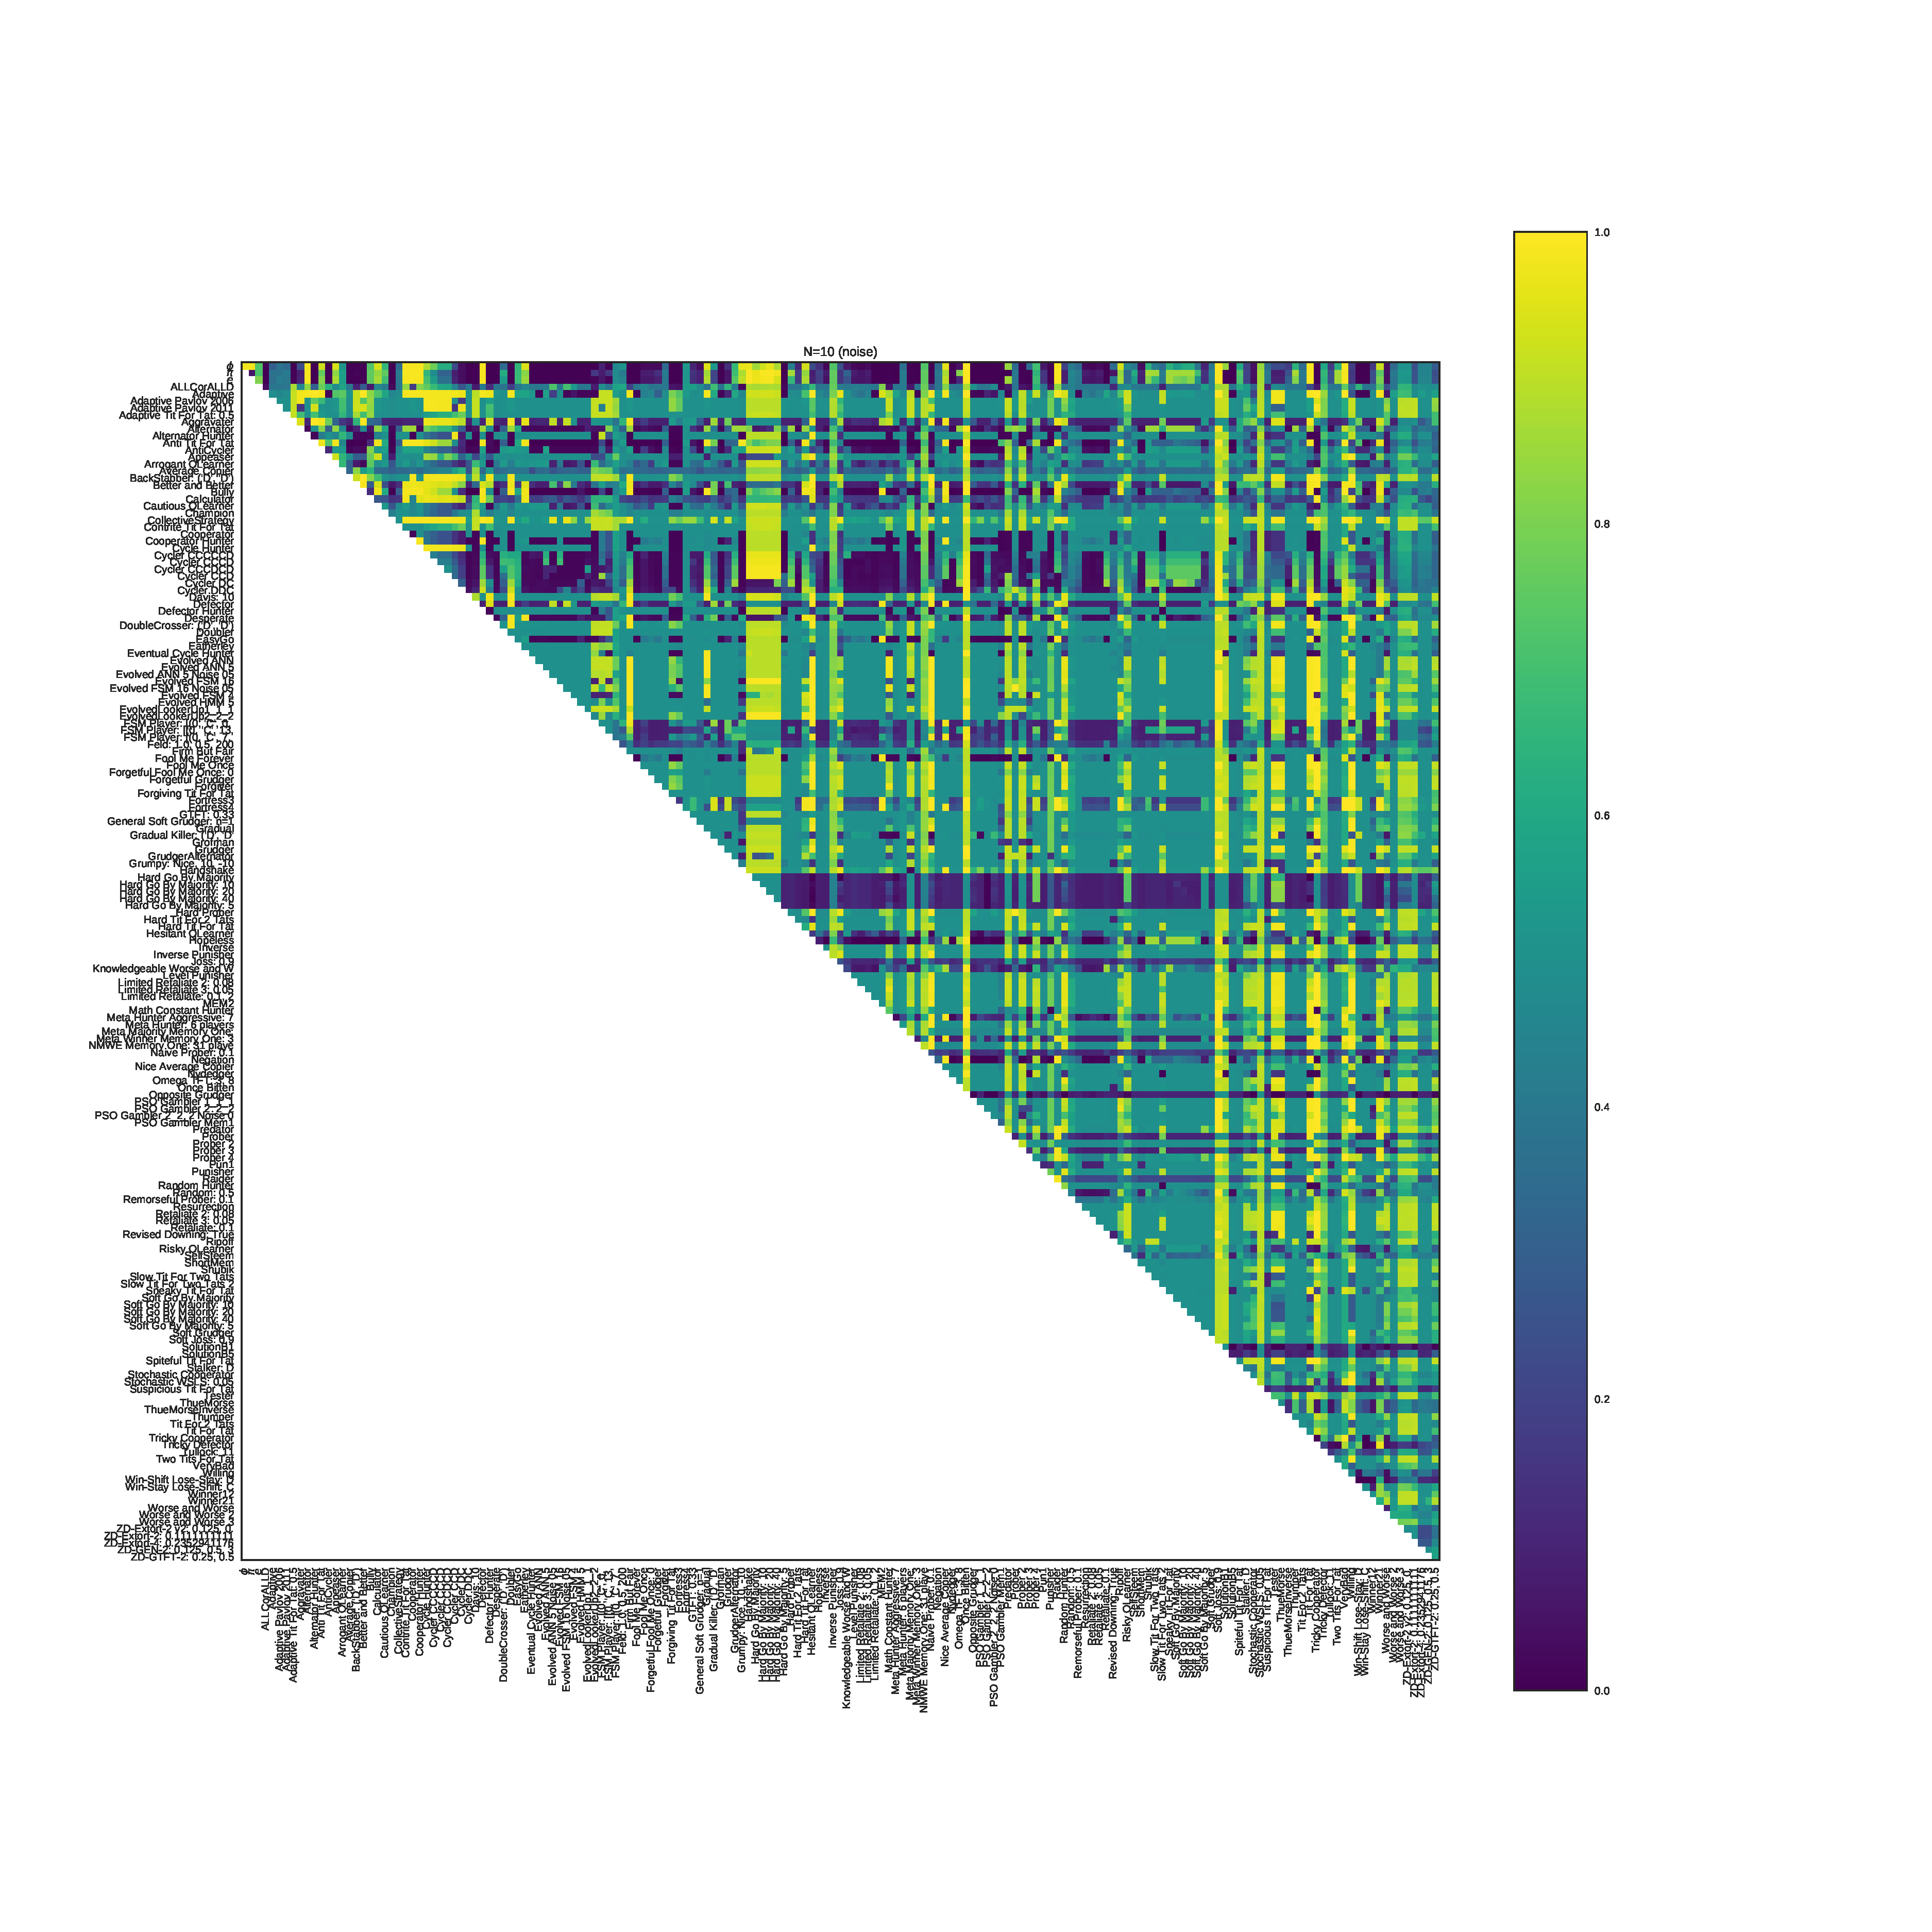
\includegraphics[width=.8\textwidth]{../img/fixation_heatmap_10_noise.pdf}
        \caption{\(N=10\)}
    \end{subfigure}%
    ~
    \begin{subfigure}[t]{.3\textwidth}
        \centering
        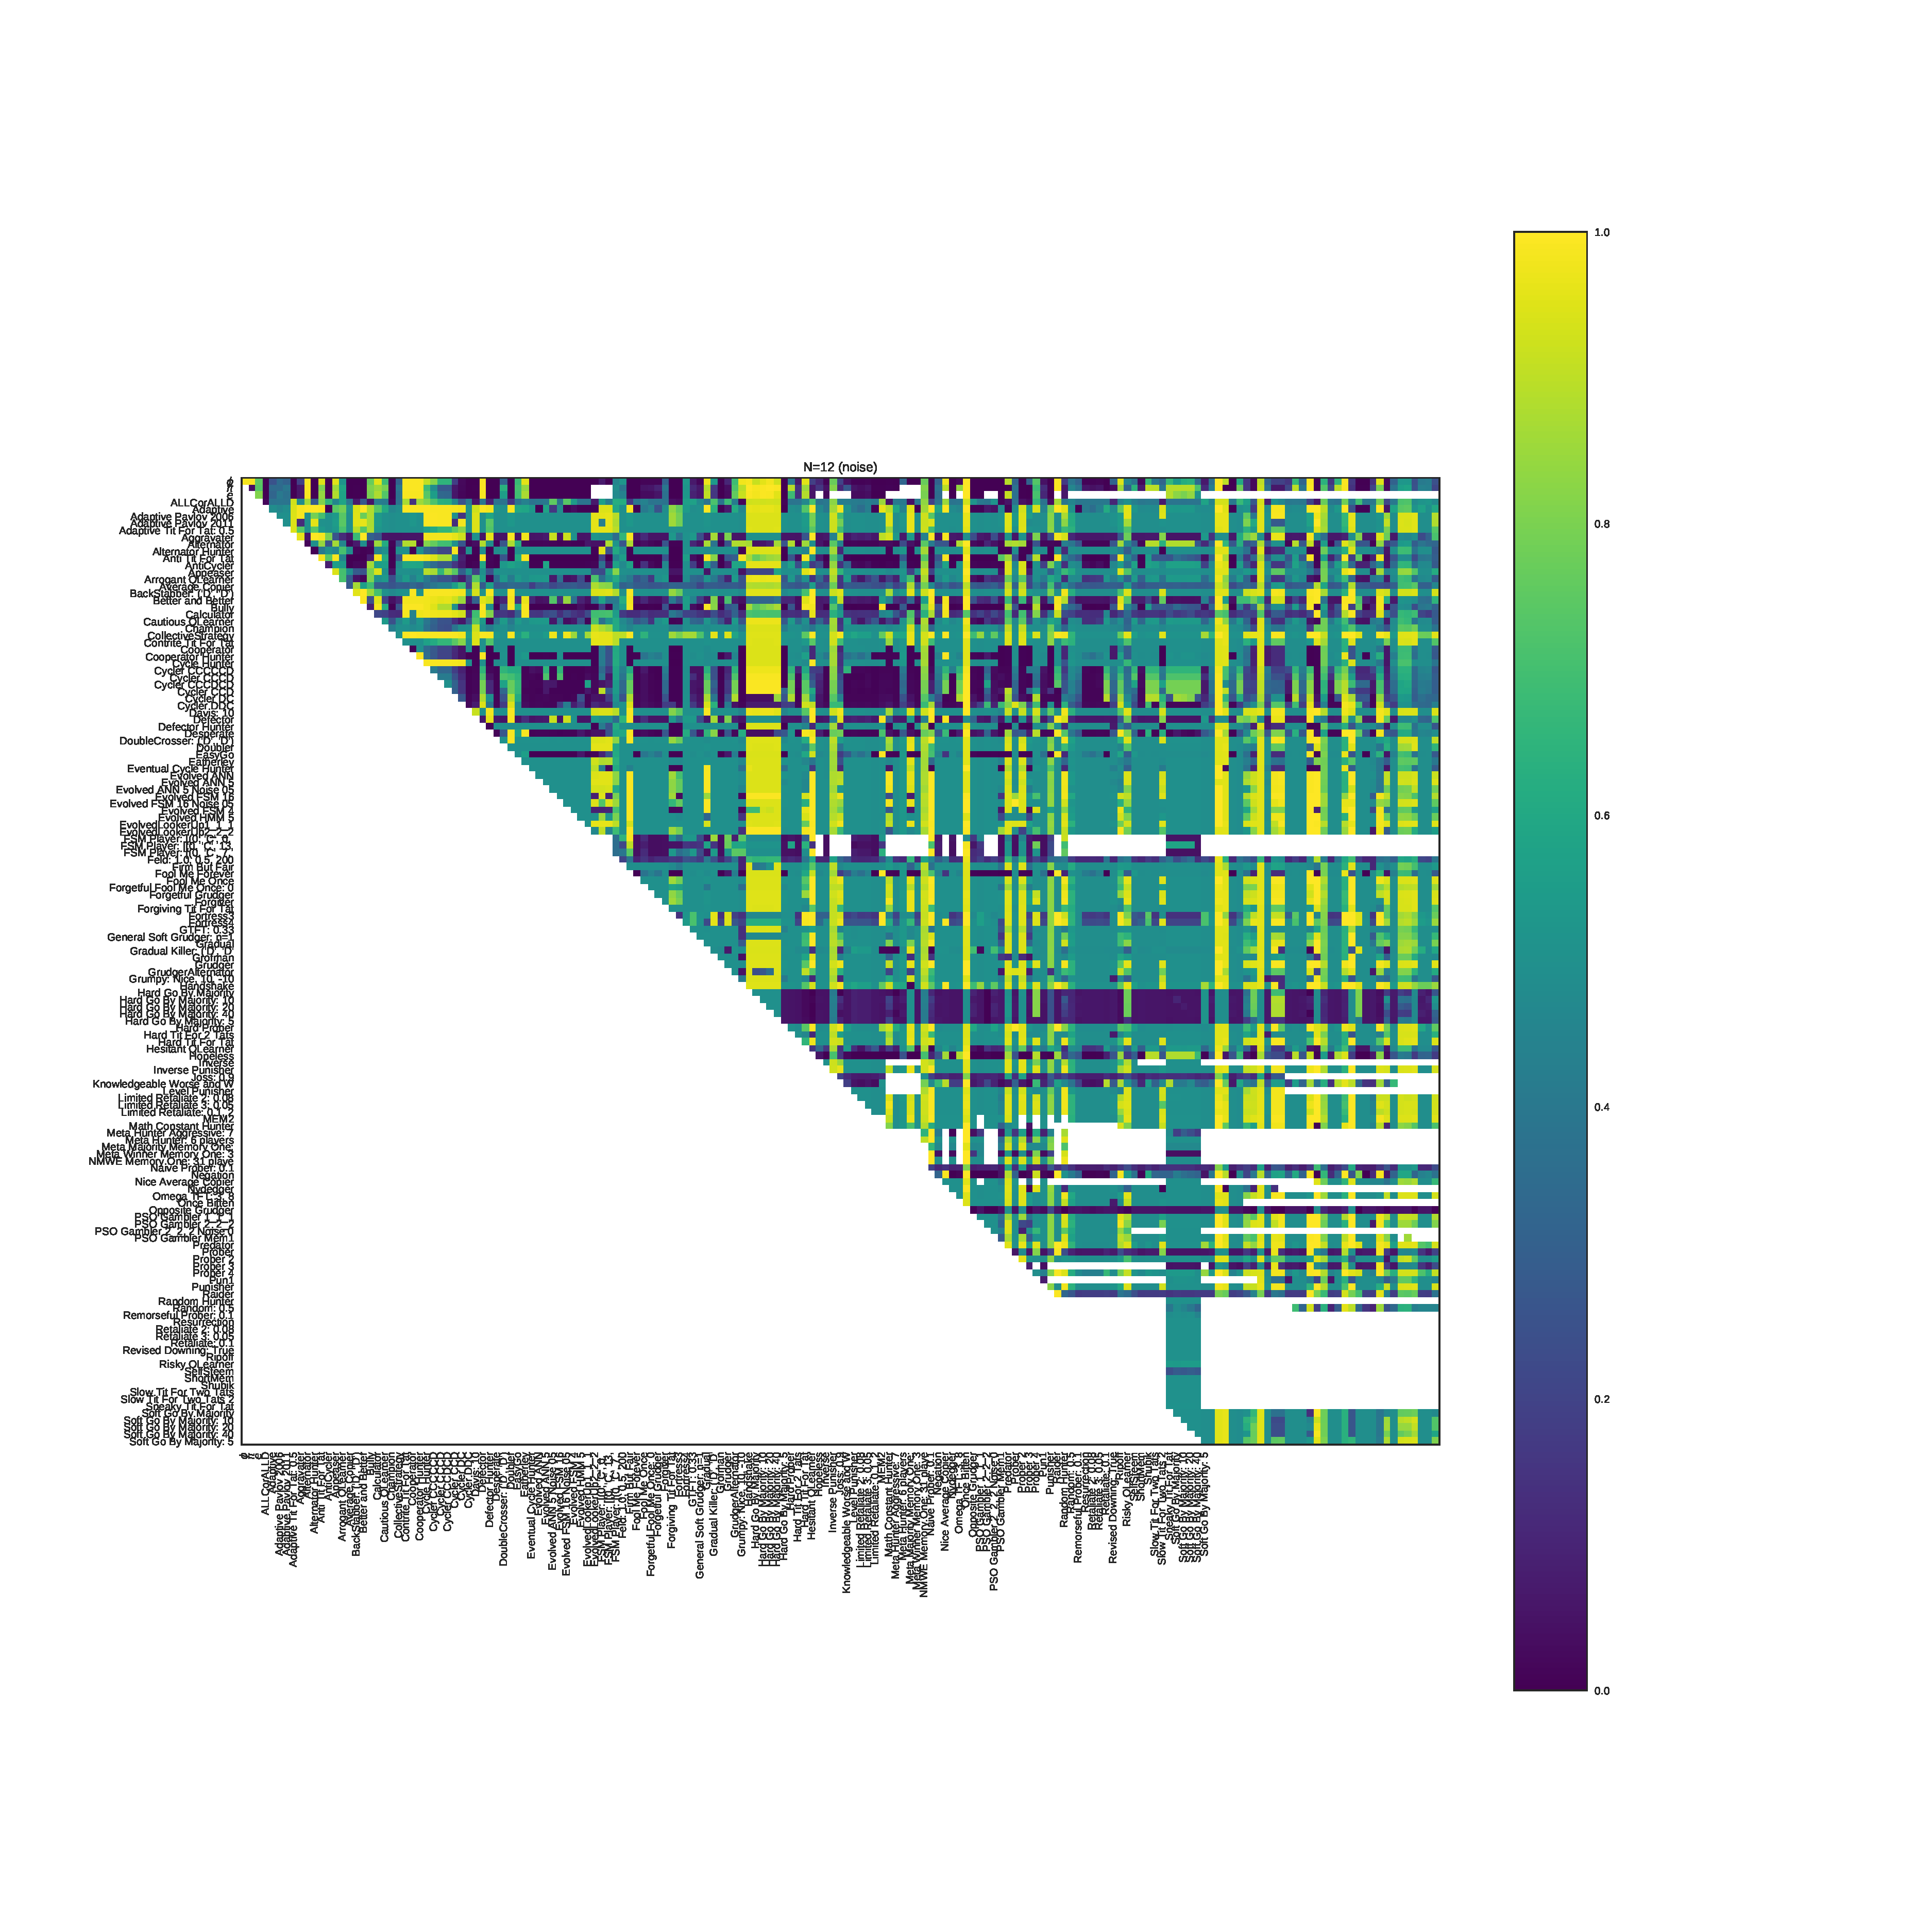
\includegraphics[width=.8\textwidth]{../img/fixation_heatmap_12_noise.pdf}
        \caption{\(N=12\)}
    \end{subfigure}%

    \begin{subfigure}[t]{.3\textwidth}
        \centering
        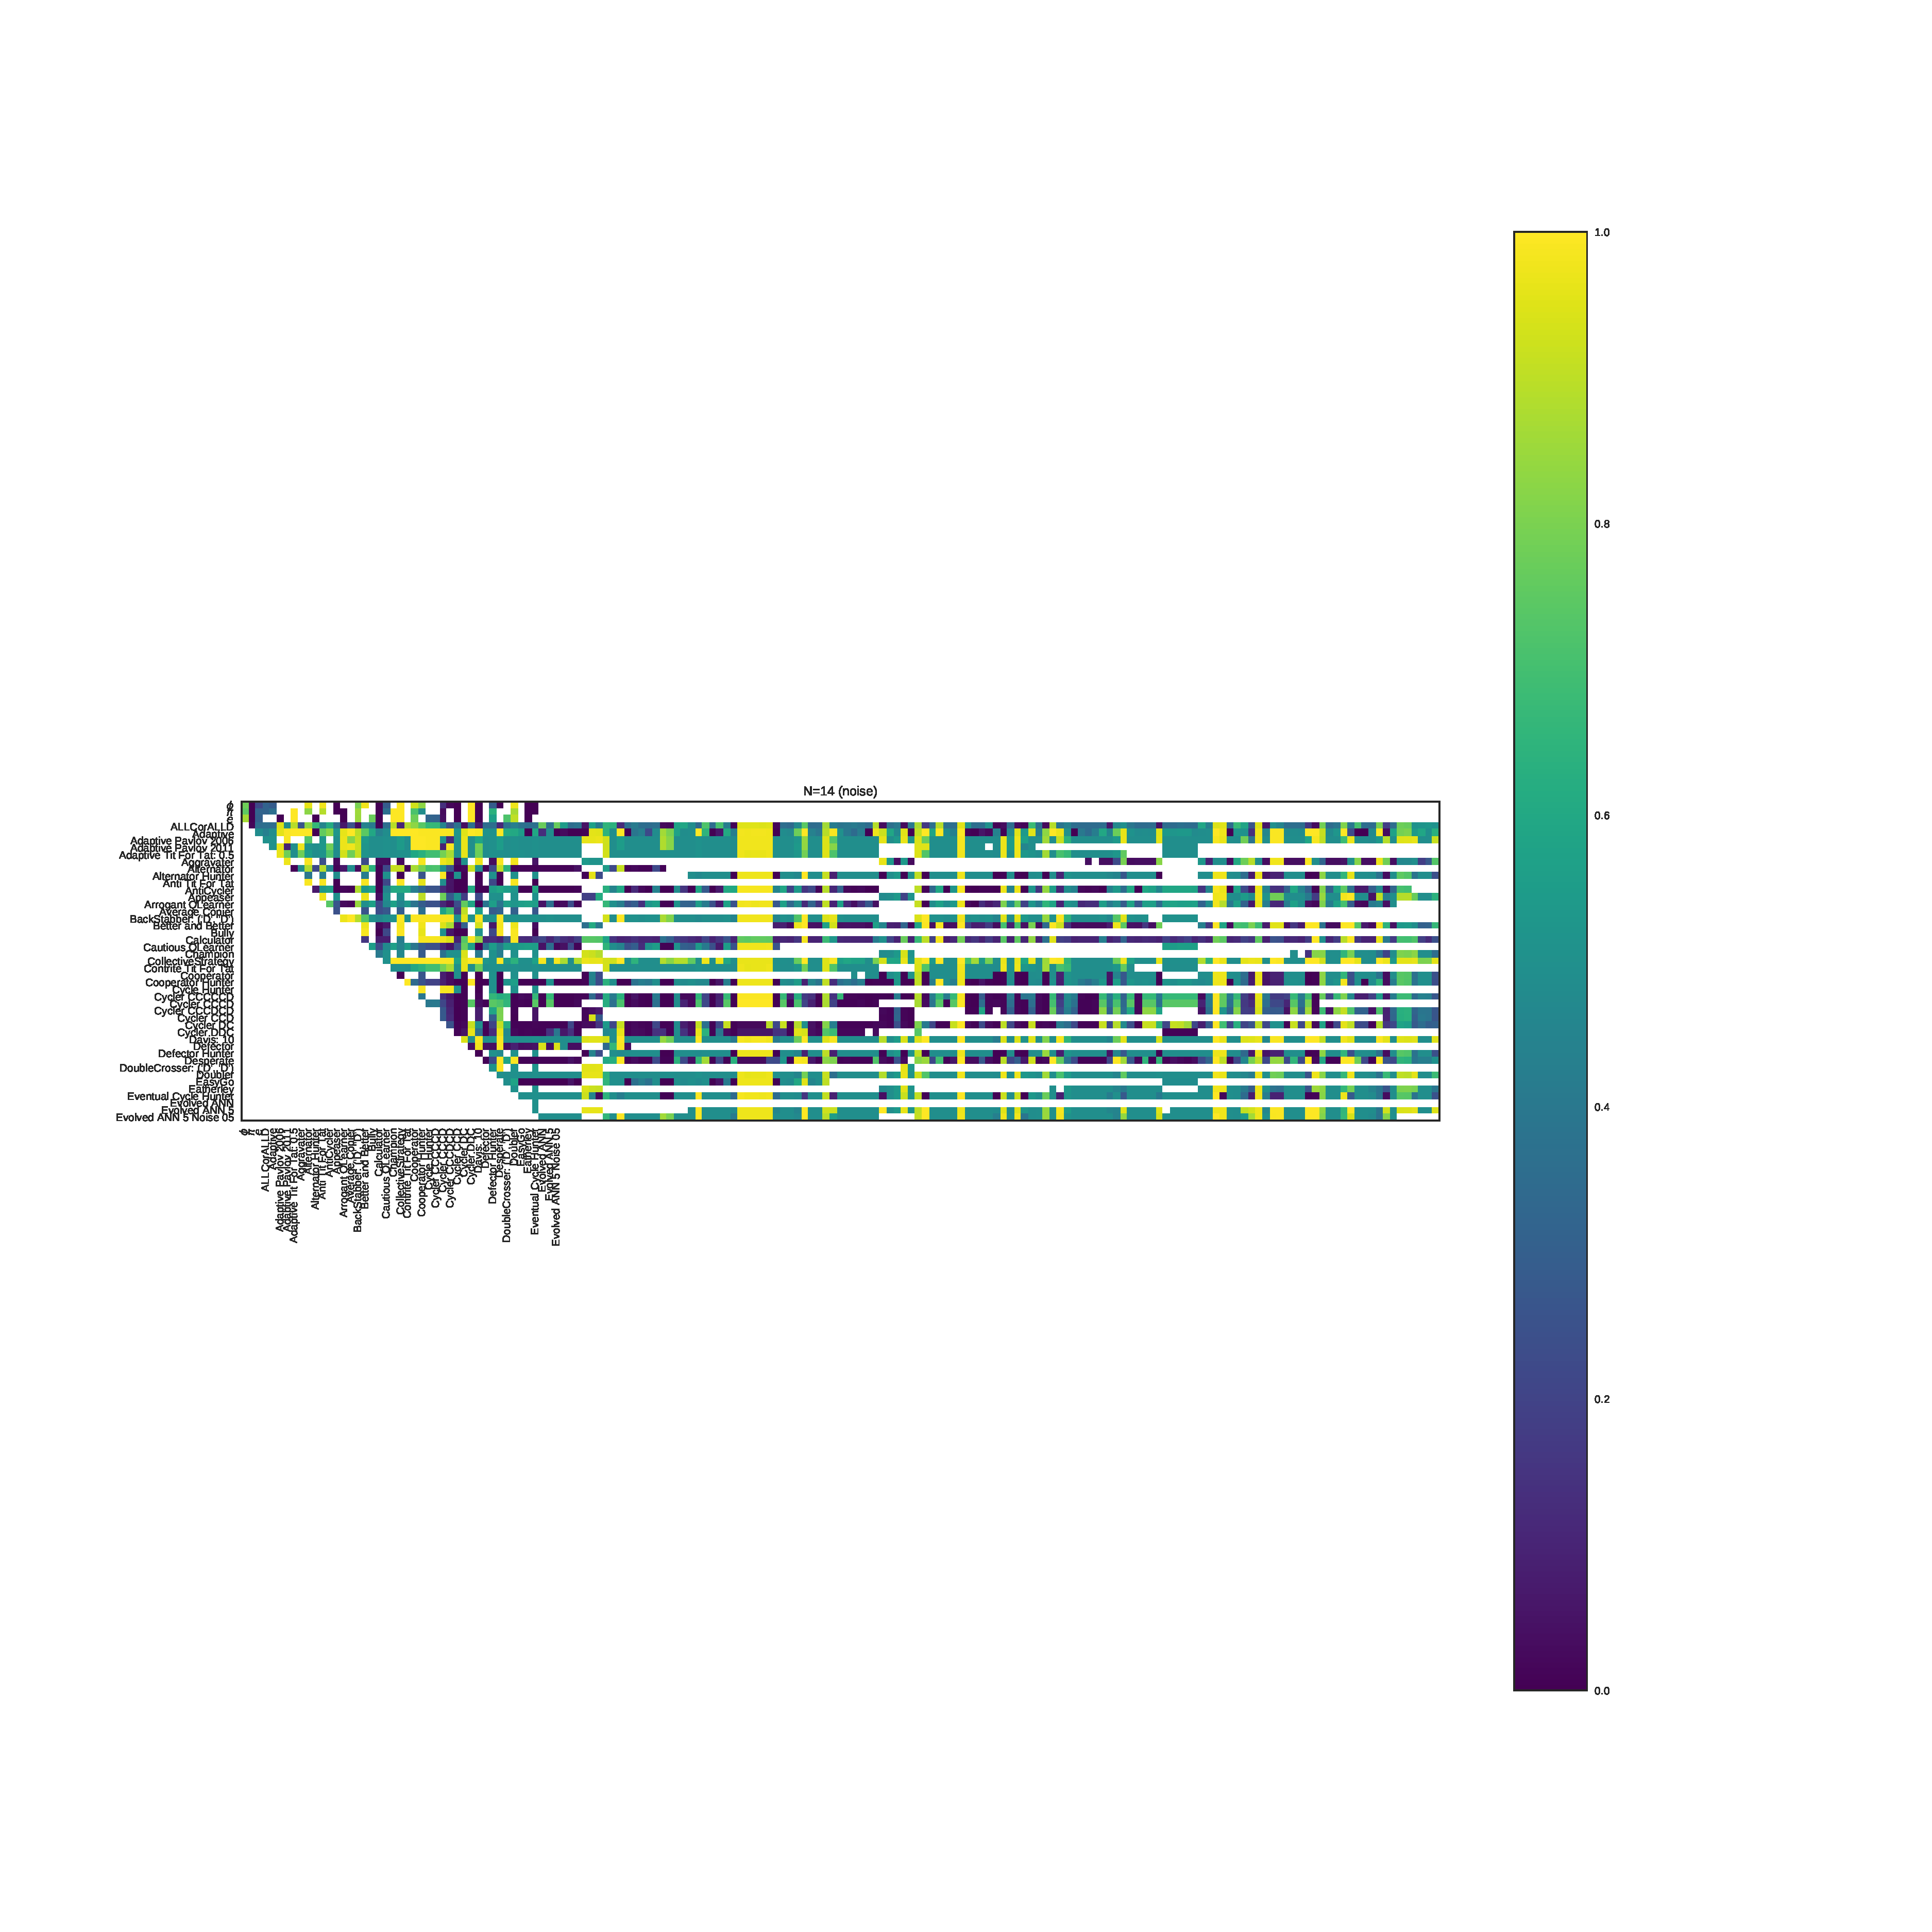
\includegraphics[width=.8\textwidth]{../img/fixation_heatmap_14_noise.pdf}
        \caption{\(N=14\)}
    \end{subfigure}%
    \caption{Pairwise fixation probabilities of all strategies (with noise)}
    \label{fig:fixation_heatmap_std}
\end{figure}

Figure~\ref{fig:histograms_all_fixation_rates_std}
and~\ref{fig:histograms_all_fixation_rates_noise} show the distribution of the
fixation rates for all strategies.

\begin{figure}[!hbtp]
    \centering
    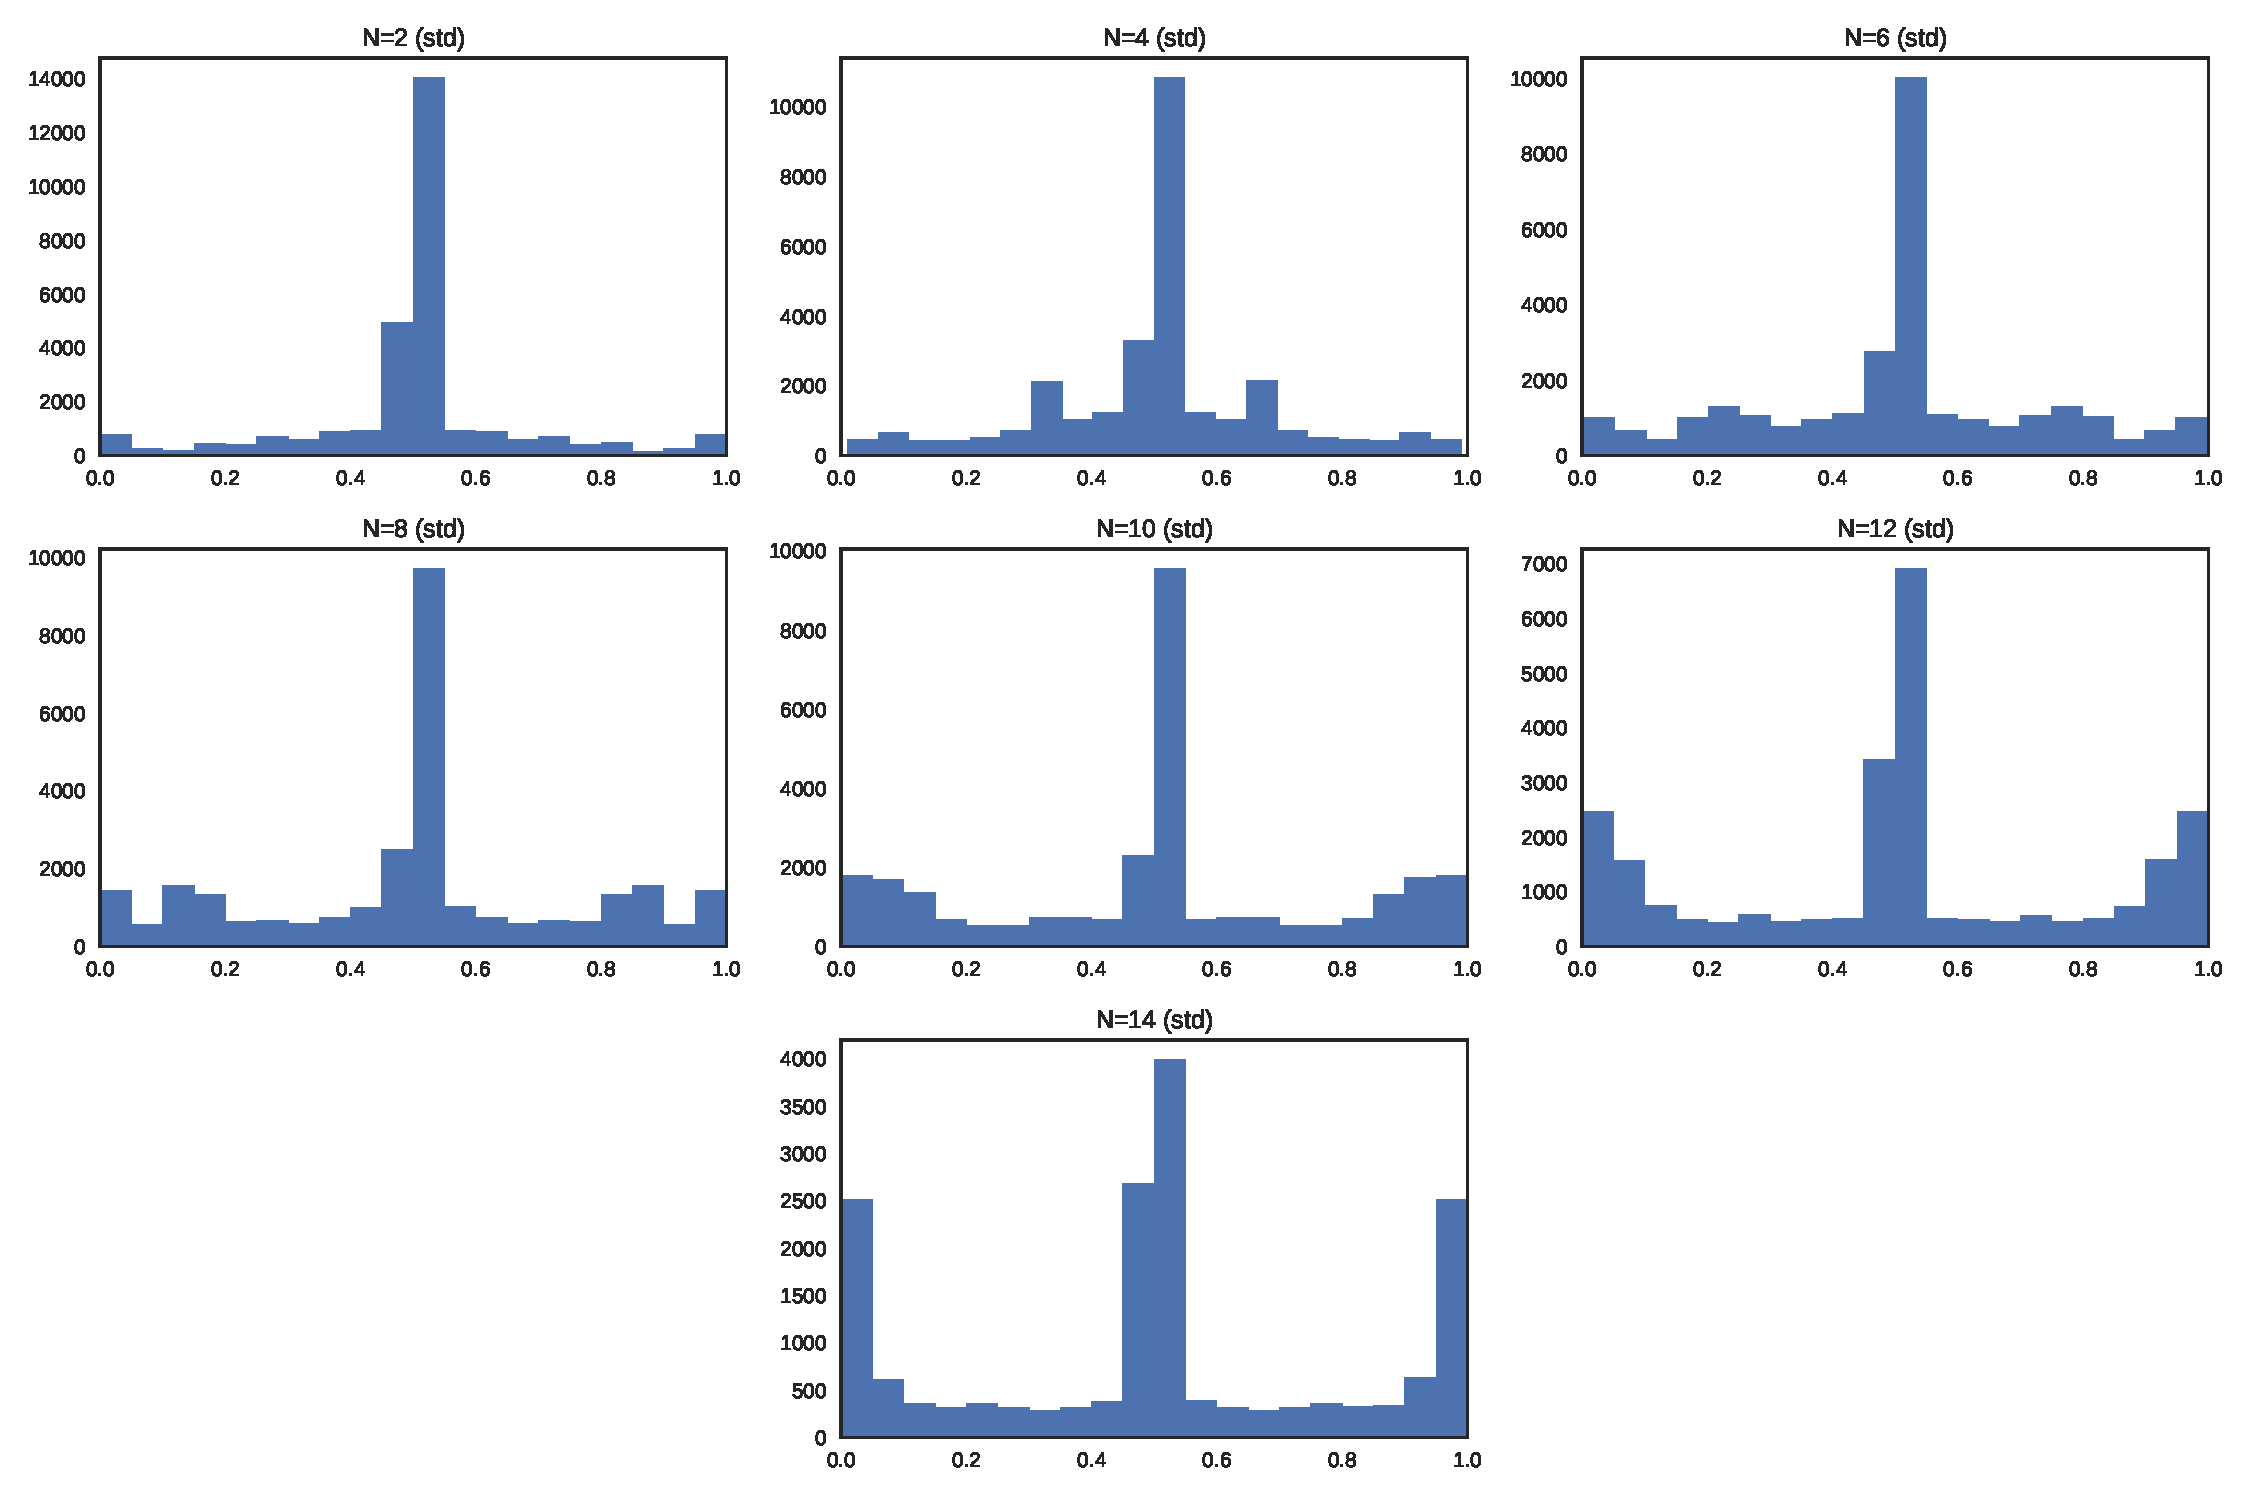
\includegraphics[width=.8\textwidth]{../img/histograms_all_fixation_rates_std.pdf}
    \caption{Distribution of fixation rates for all players}
\end{figure}

\begin{figure}[!hbtp]
    \centering
    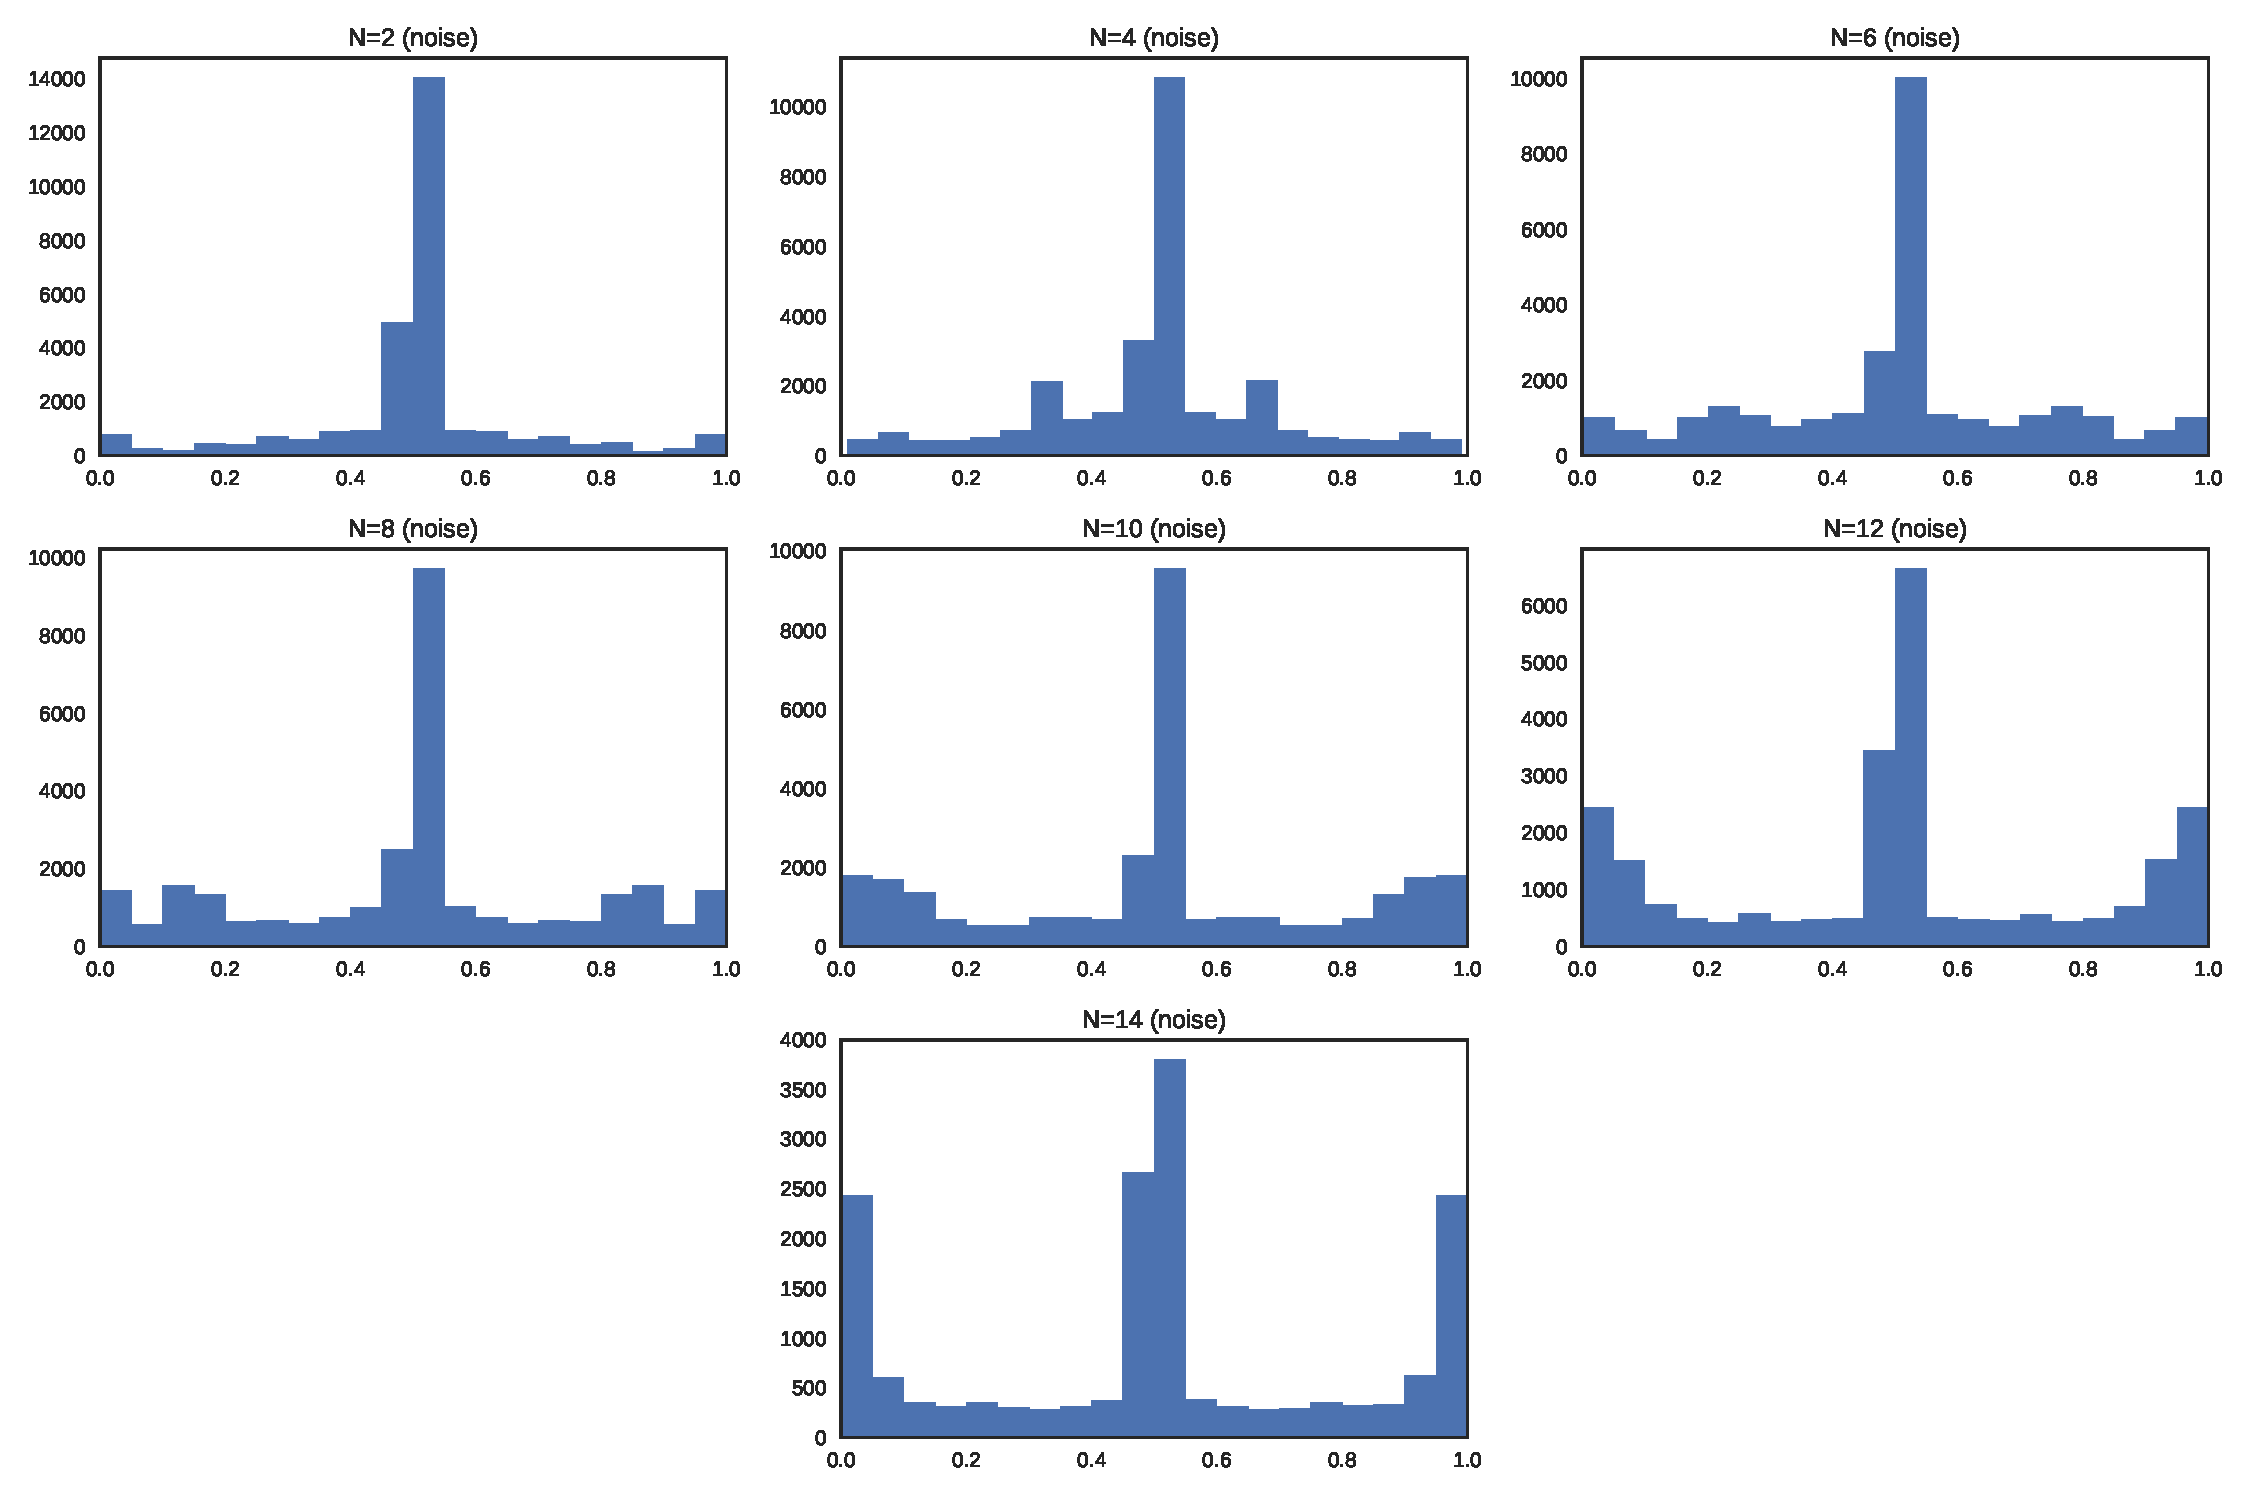
\includegraphics[width=.8\textwidth]{../img/histograms_all_fixation_rates_noise.pdf}
    \caption{Distribution of fixation rates for all players (noise)}
\end{figure}

\begin{figure}[!hbtp]
    \centering
    \begin{subfigure}[t]{\textwidth}
        \centering
        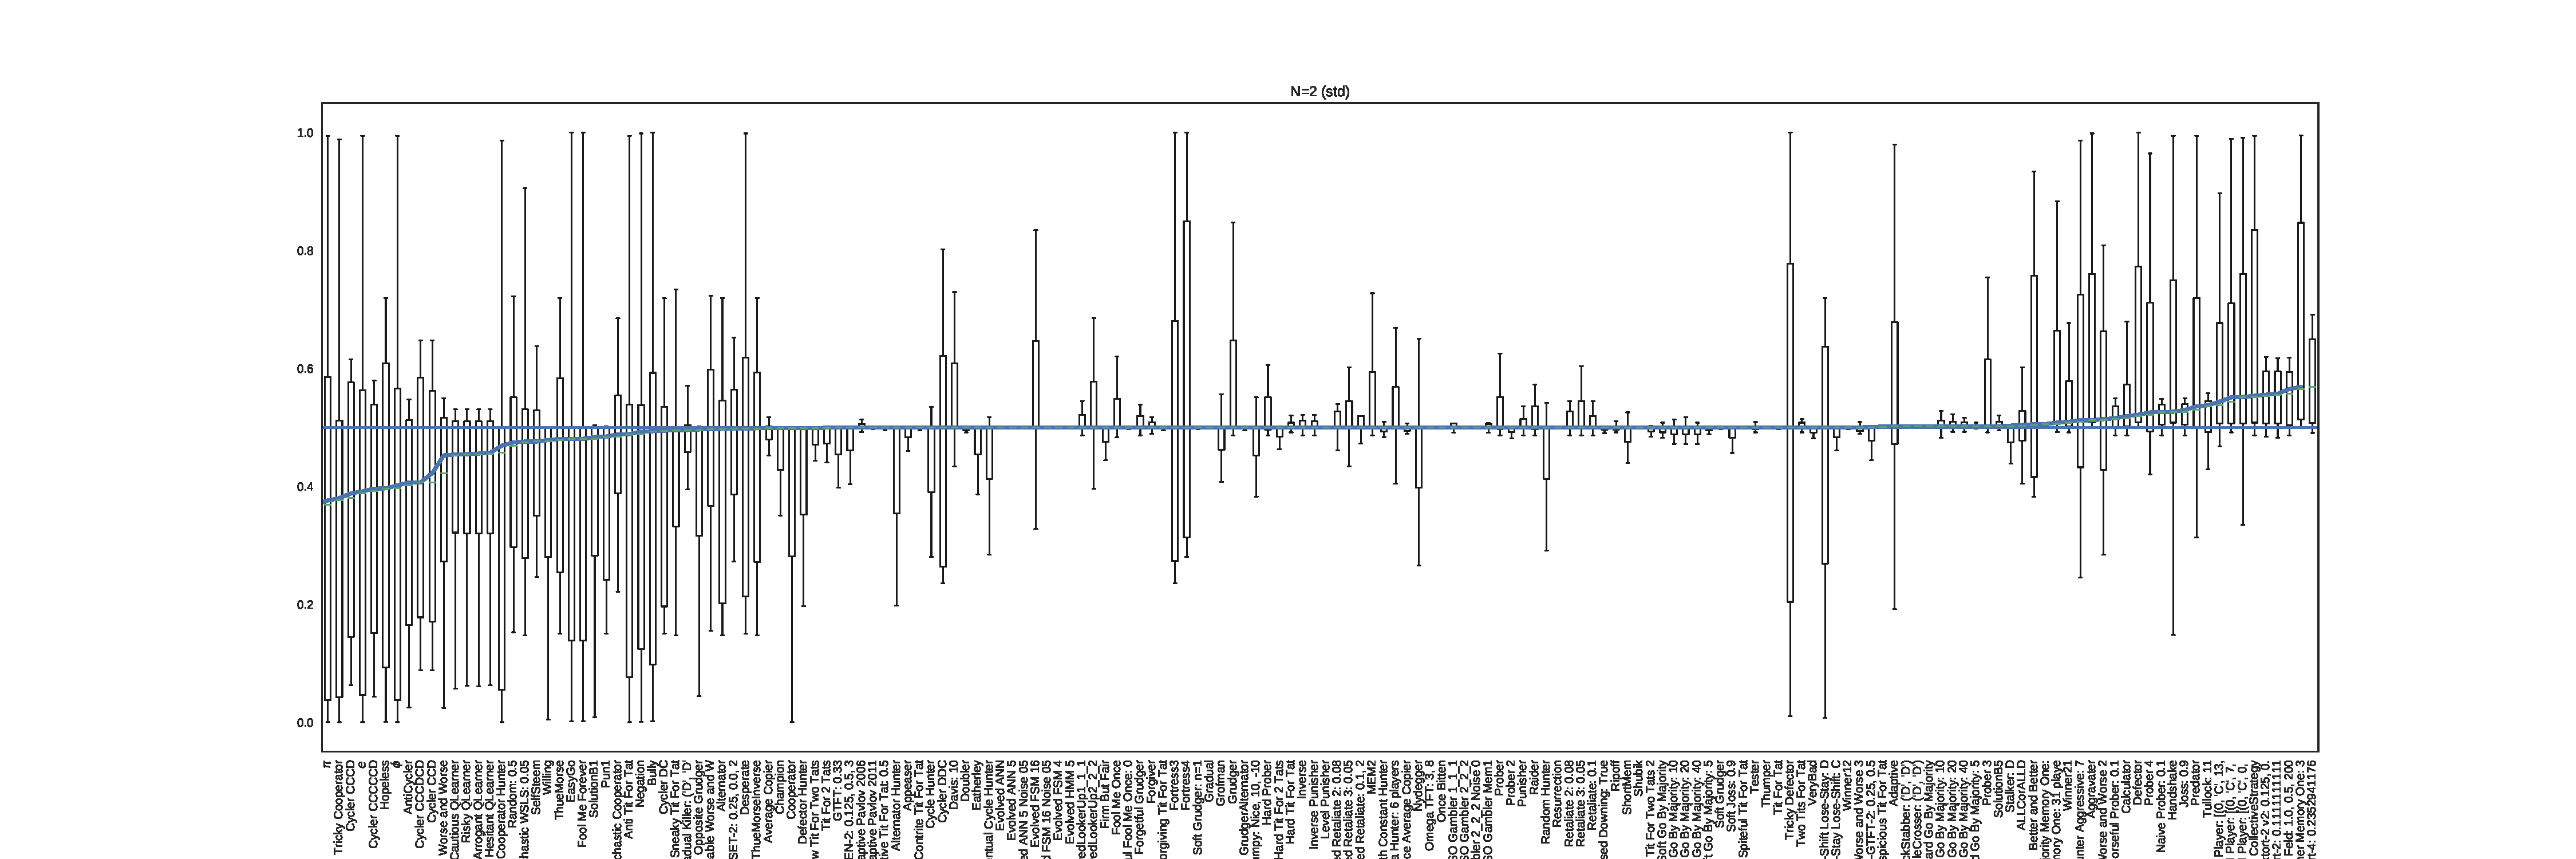
\includegraphics[width=\textwidth]{../img/fixation_boxplot_2_std.pdf}
        \caption{\(N=2\)}
    \end{subfigure}%

    %\begin{subfigure}[t]{\textwidth}
        %\centering
        %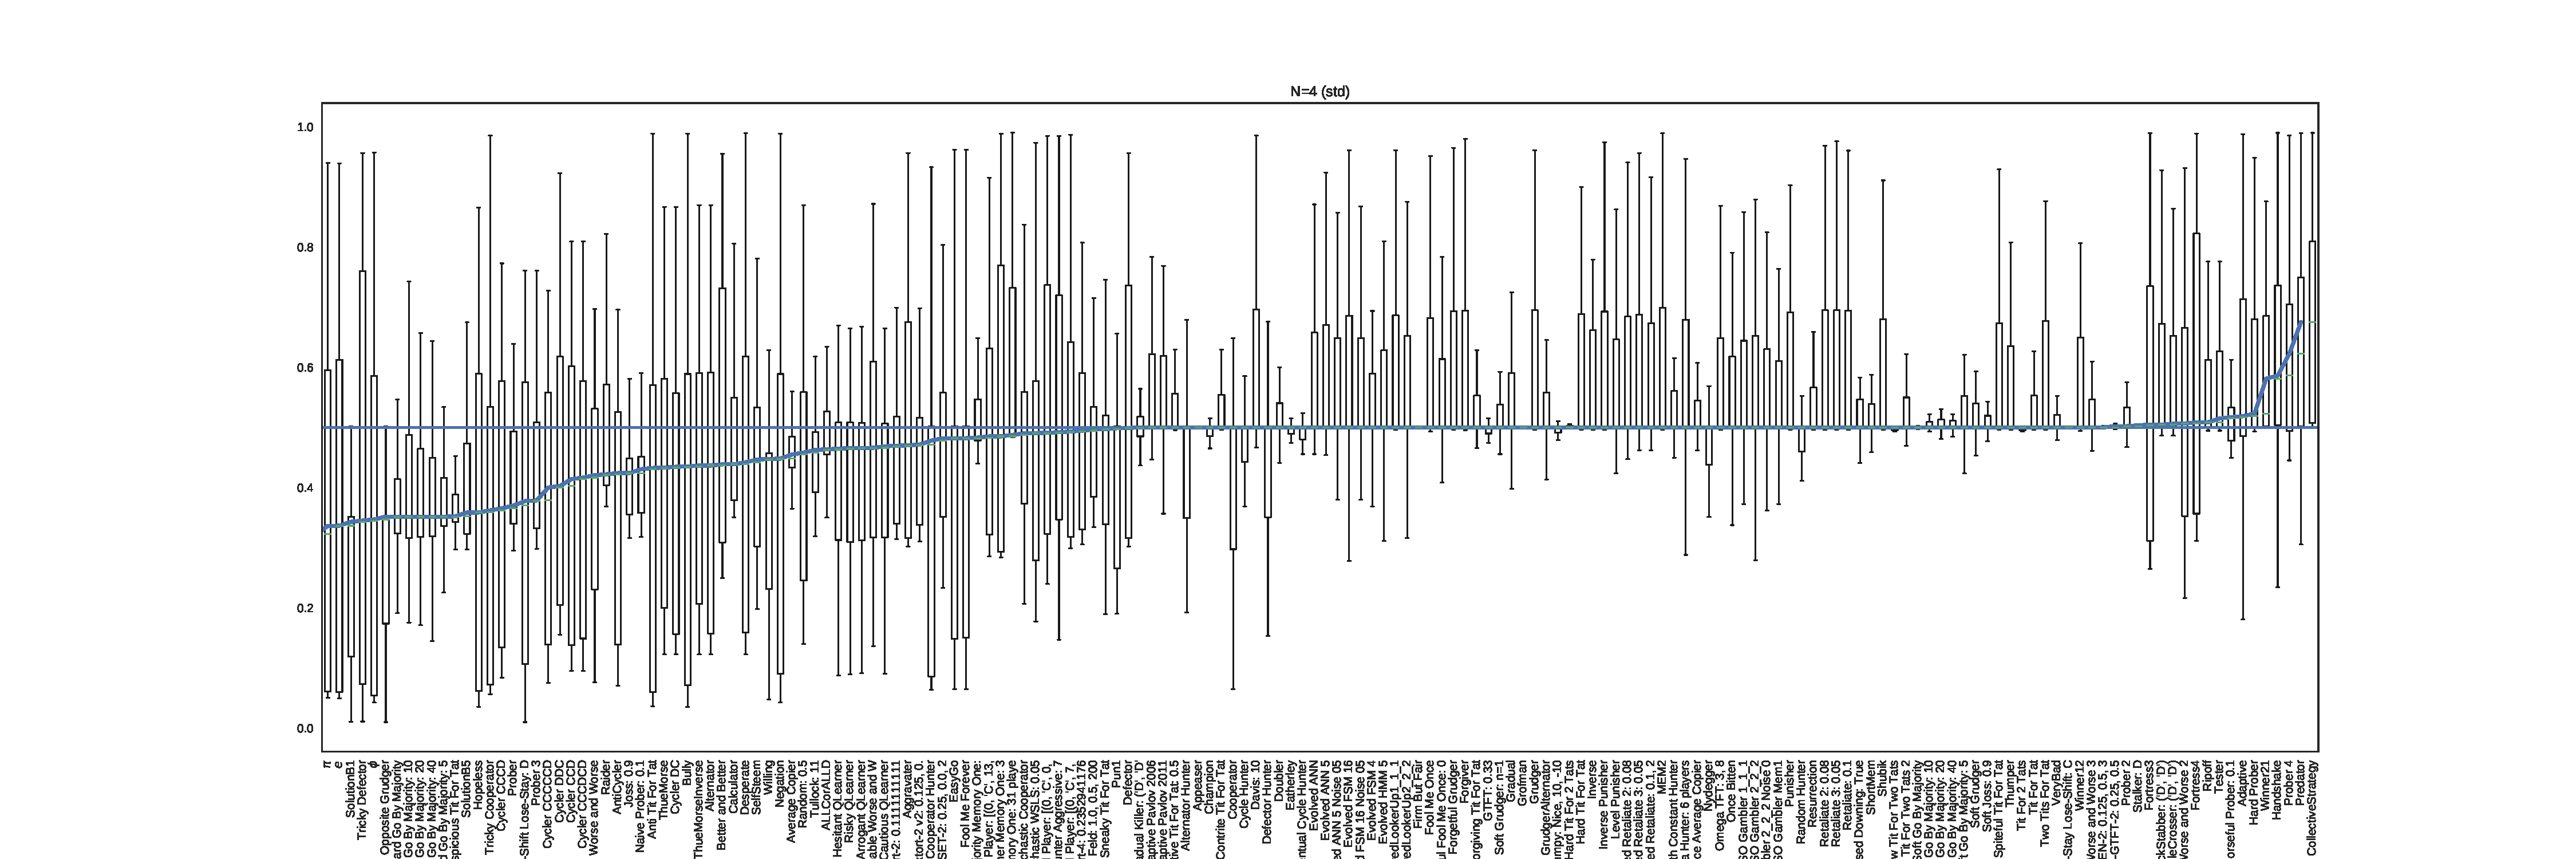
\includegraphics[width=\textwidth]{../img/fixation_boxplot_4_std.pdf}
        %\caption{\(N=4\)}
    %\end{subfigure}%

    %\begin{subfigure}[t]{\textwidth}
        %\centering
        %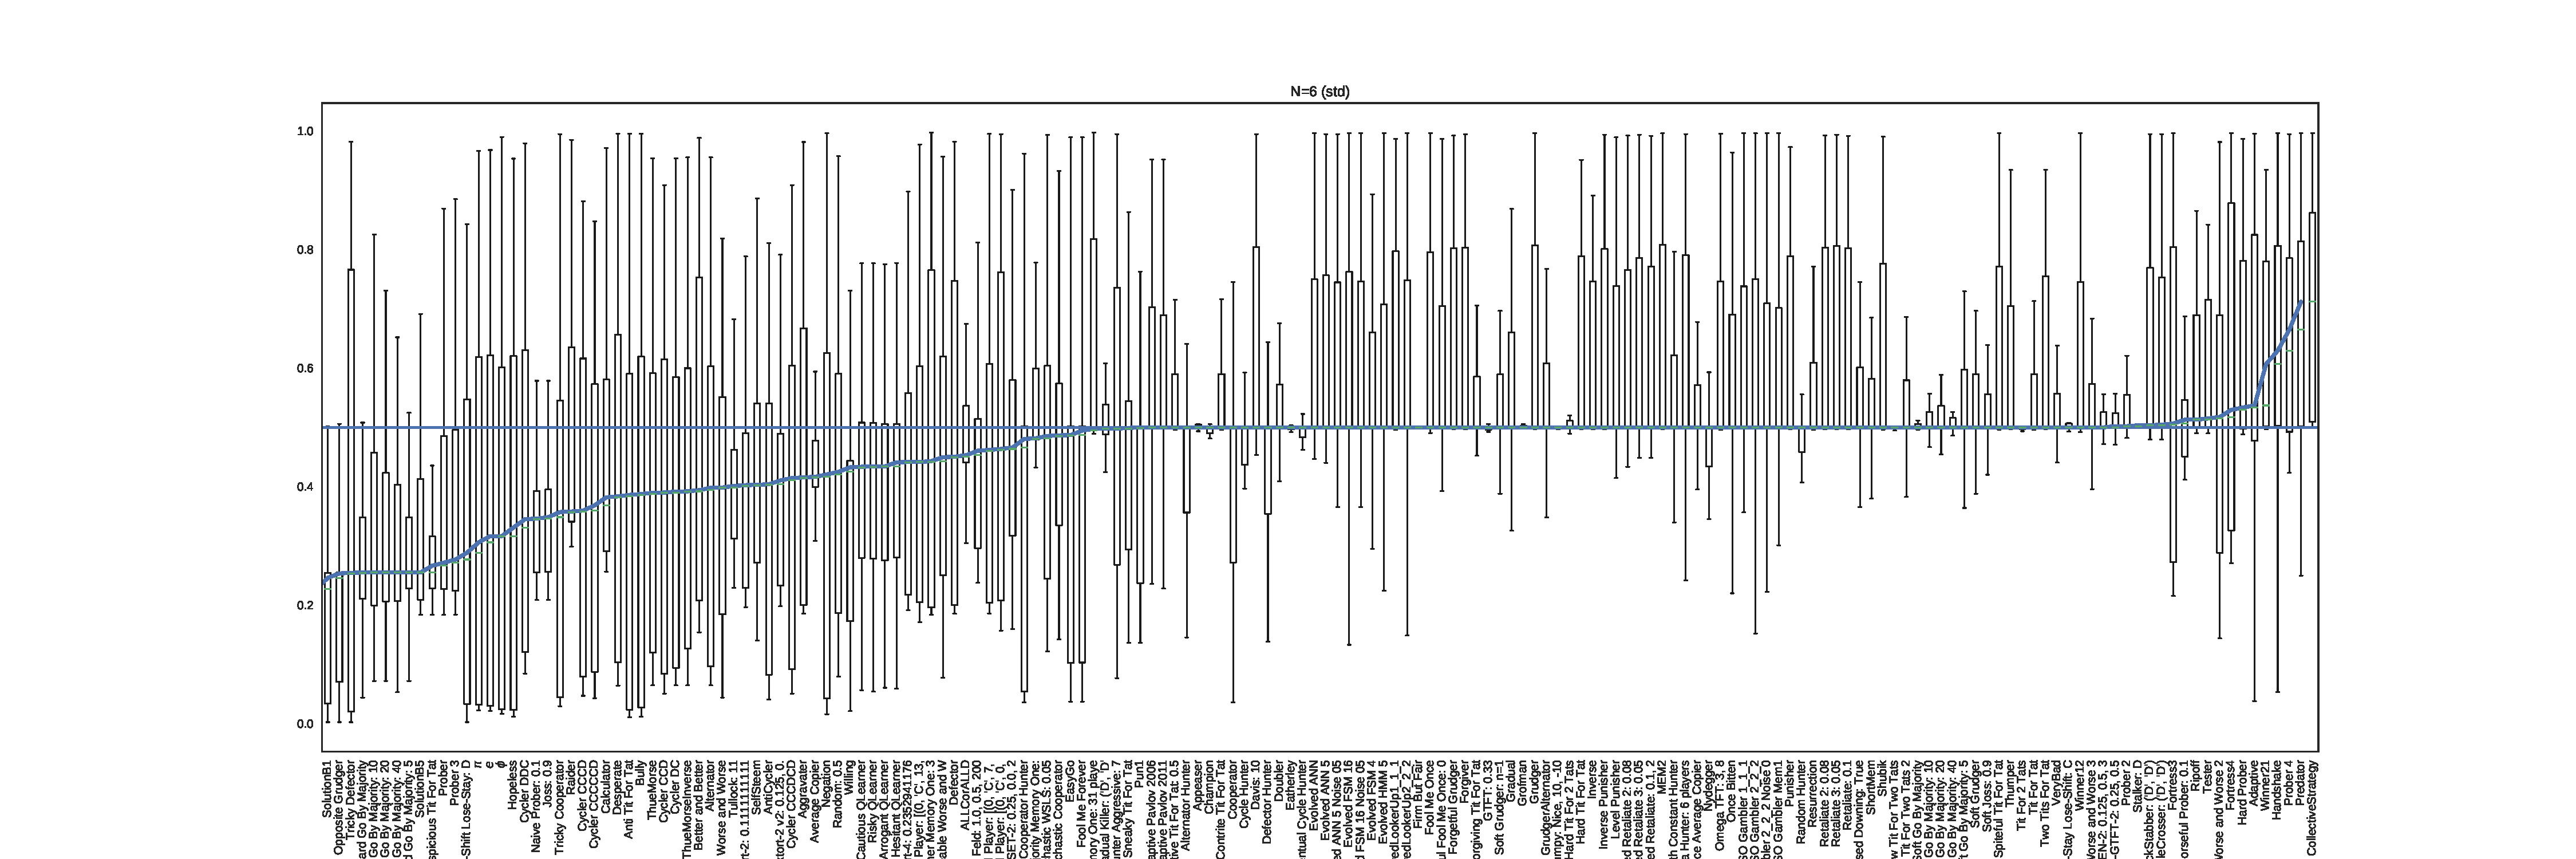
\includegraphics[width=\textwidth]{../img/fixation_boxplot_6_std.pdf}
        %\caption{\(N=6\)}
    %\end{subfigure}%

    \begin{subfigure}[t]{\textwidth}
        \centering
        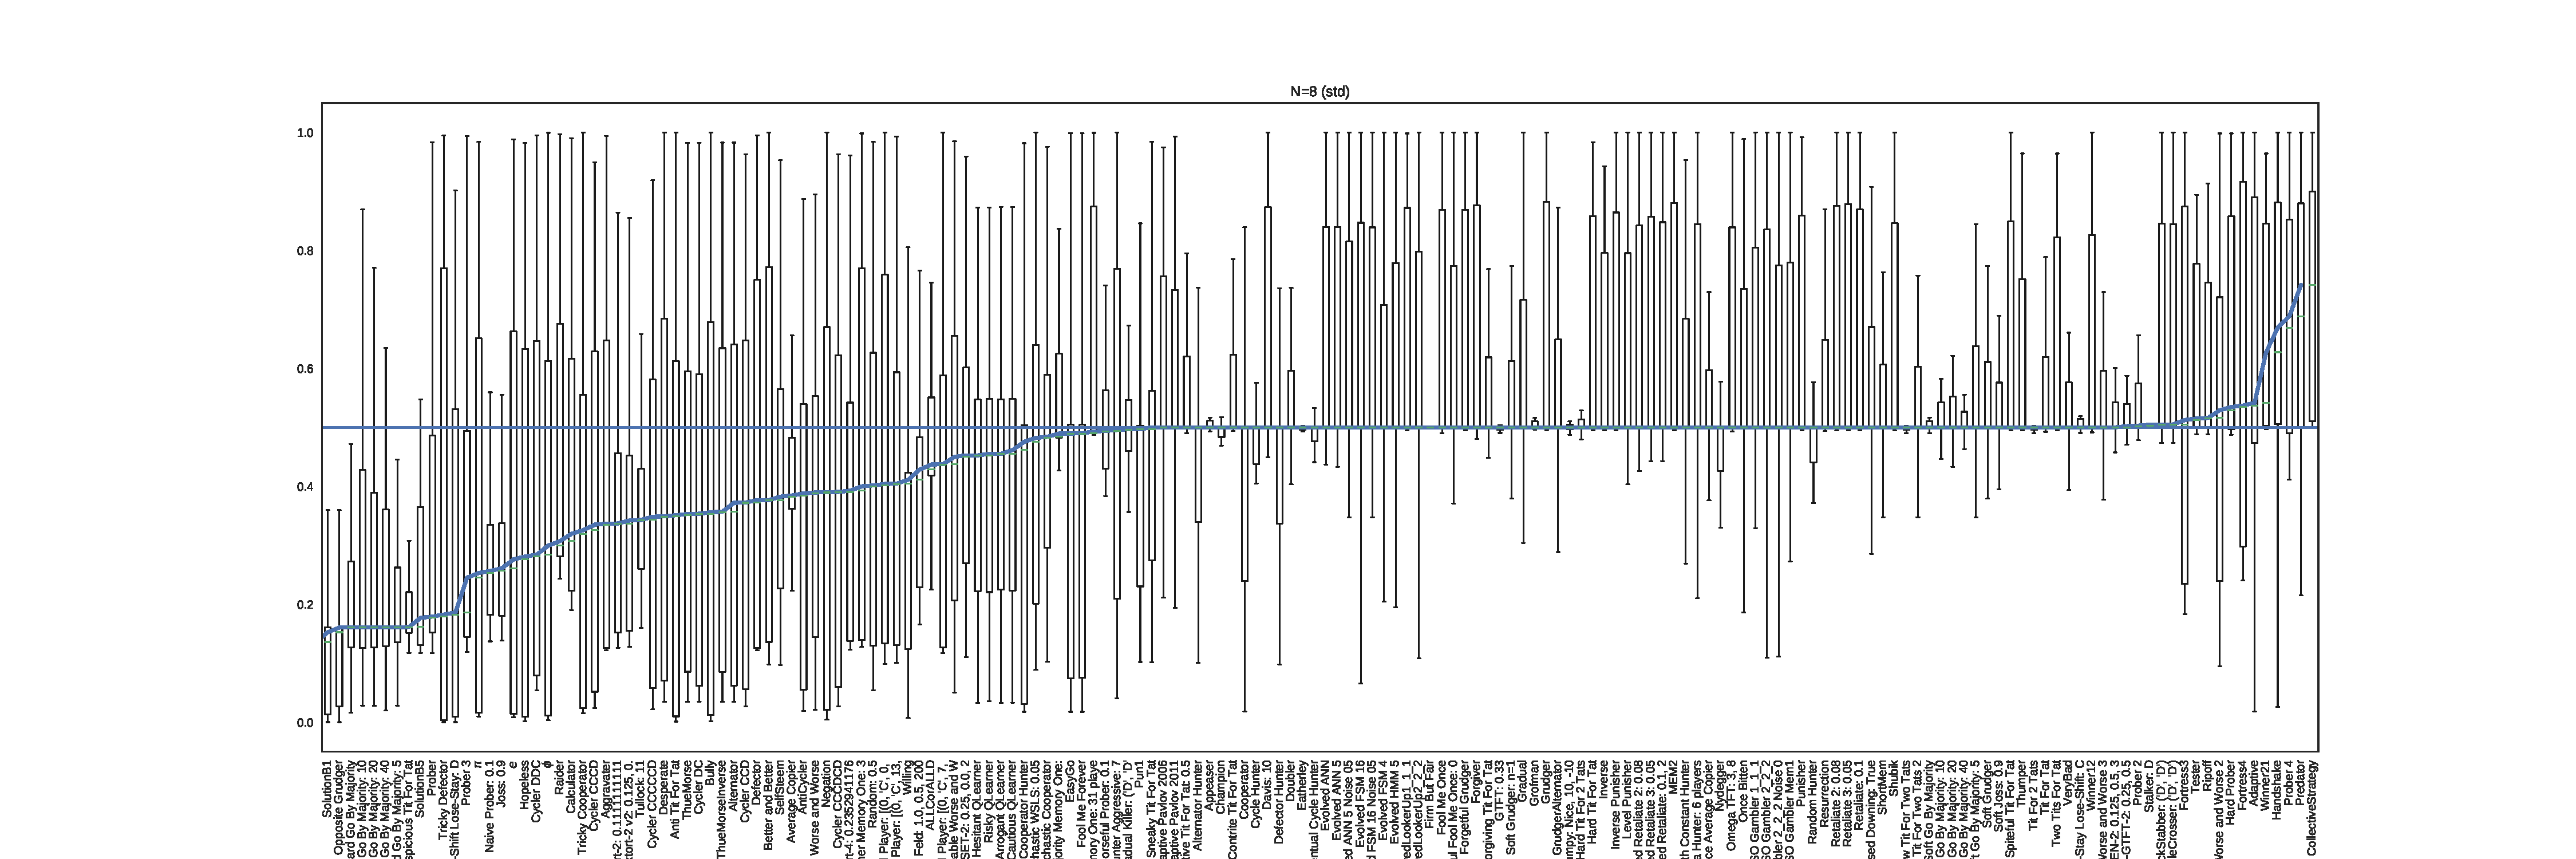
\includegraphics[width=\textwidth]{../img/fixation_boxplot_8_std.pdf}
        \caption{\(N=8\)}
    \end{subfigure}%

    %\begin{subfigure}[t]{\textwidth}
        %\centering
        %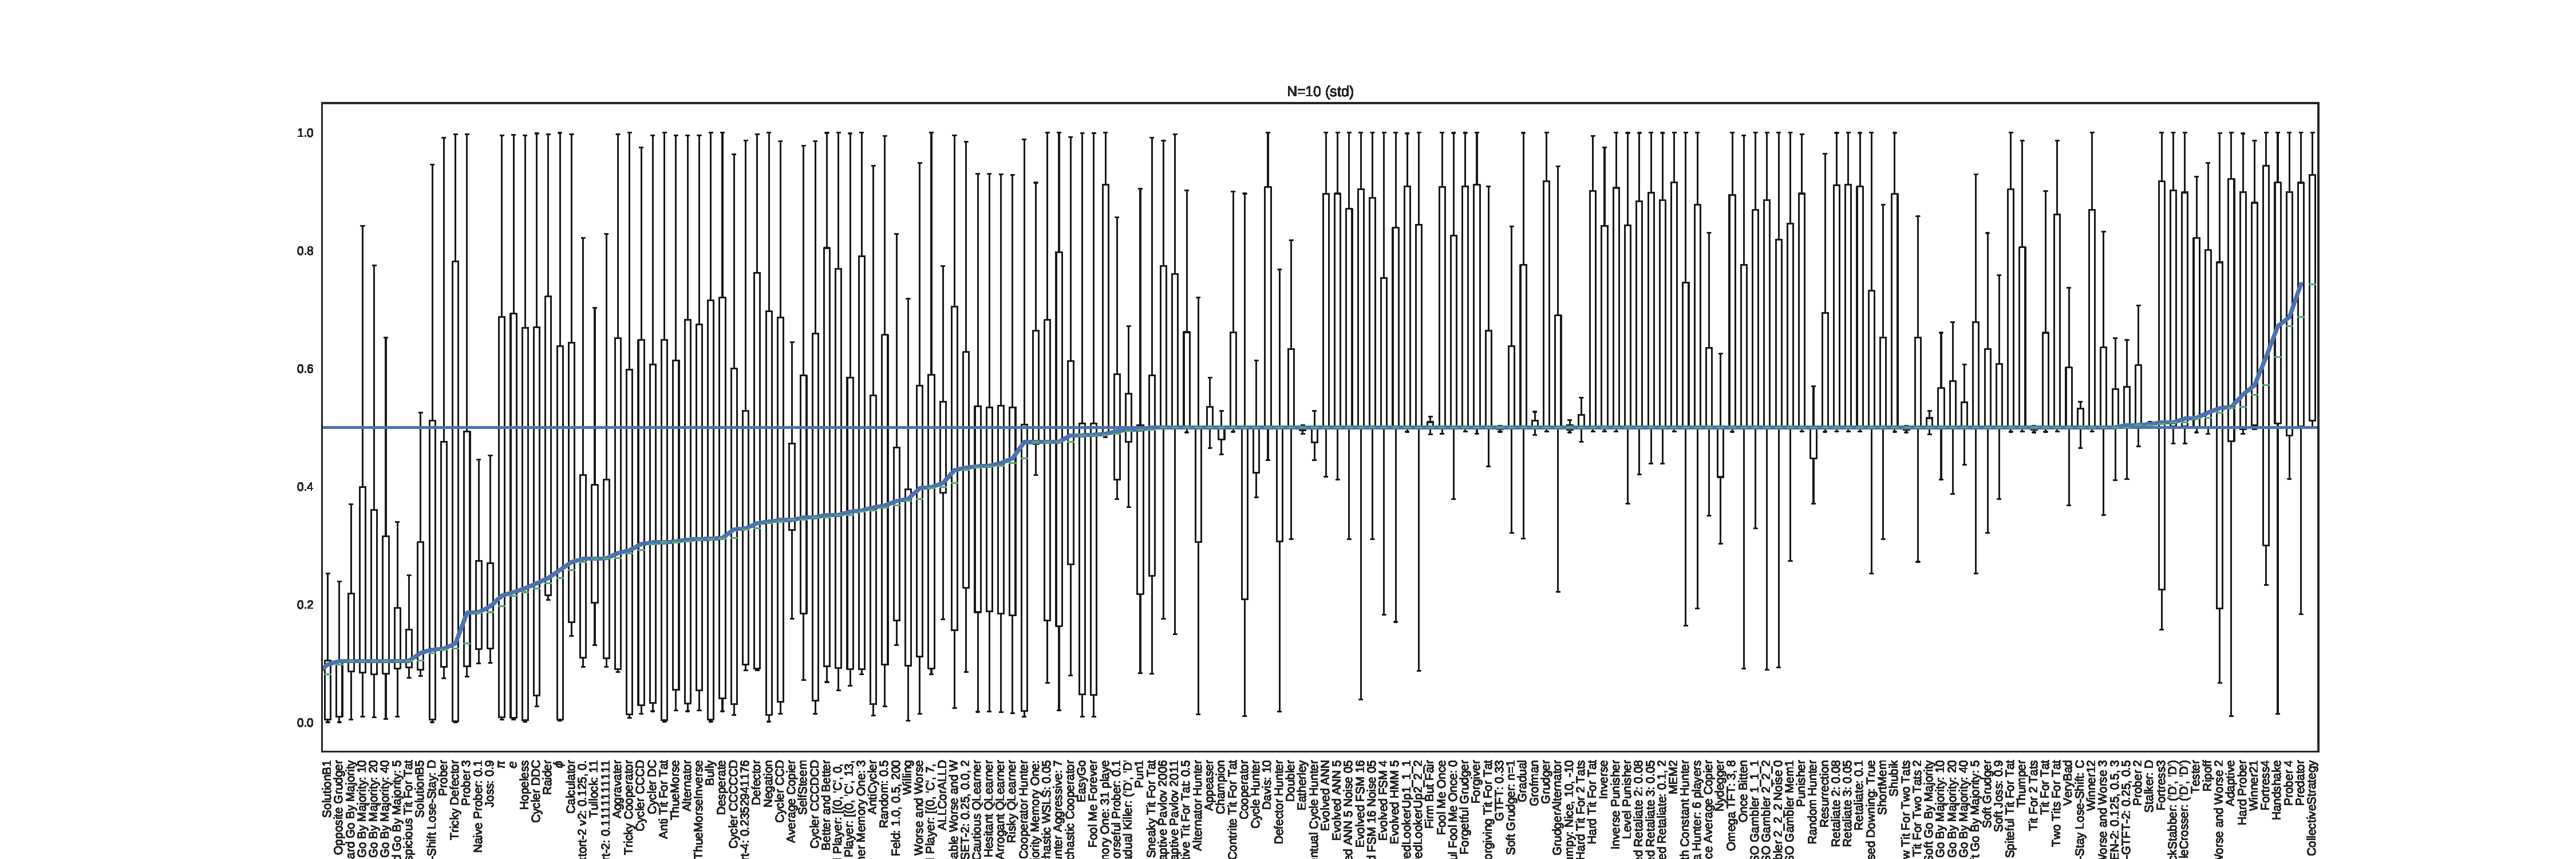
\includegraphics[width=\textwidth]{../img/fixation_boxplot_10_std.pdf}
        %\caption{\(N=10\)}
    %\end{subfigure}%

    %\begin{subfigure}[t]{\textwidth}
        %\centering
        %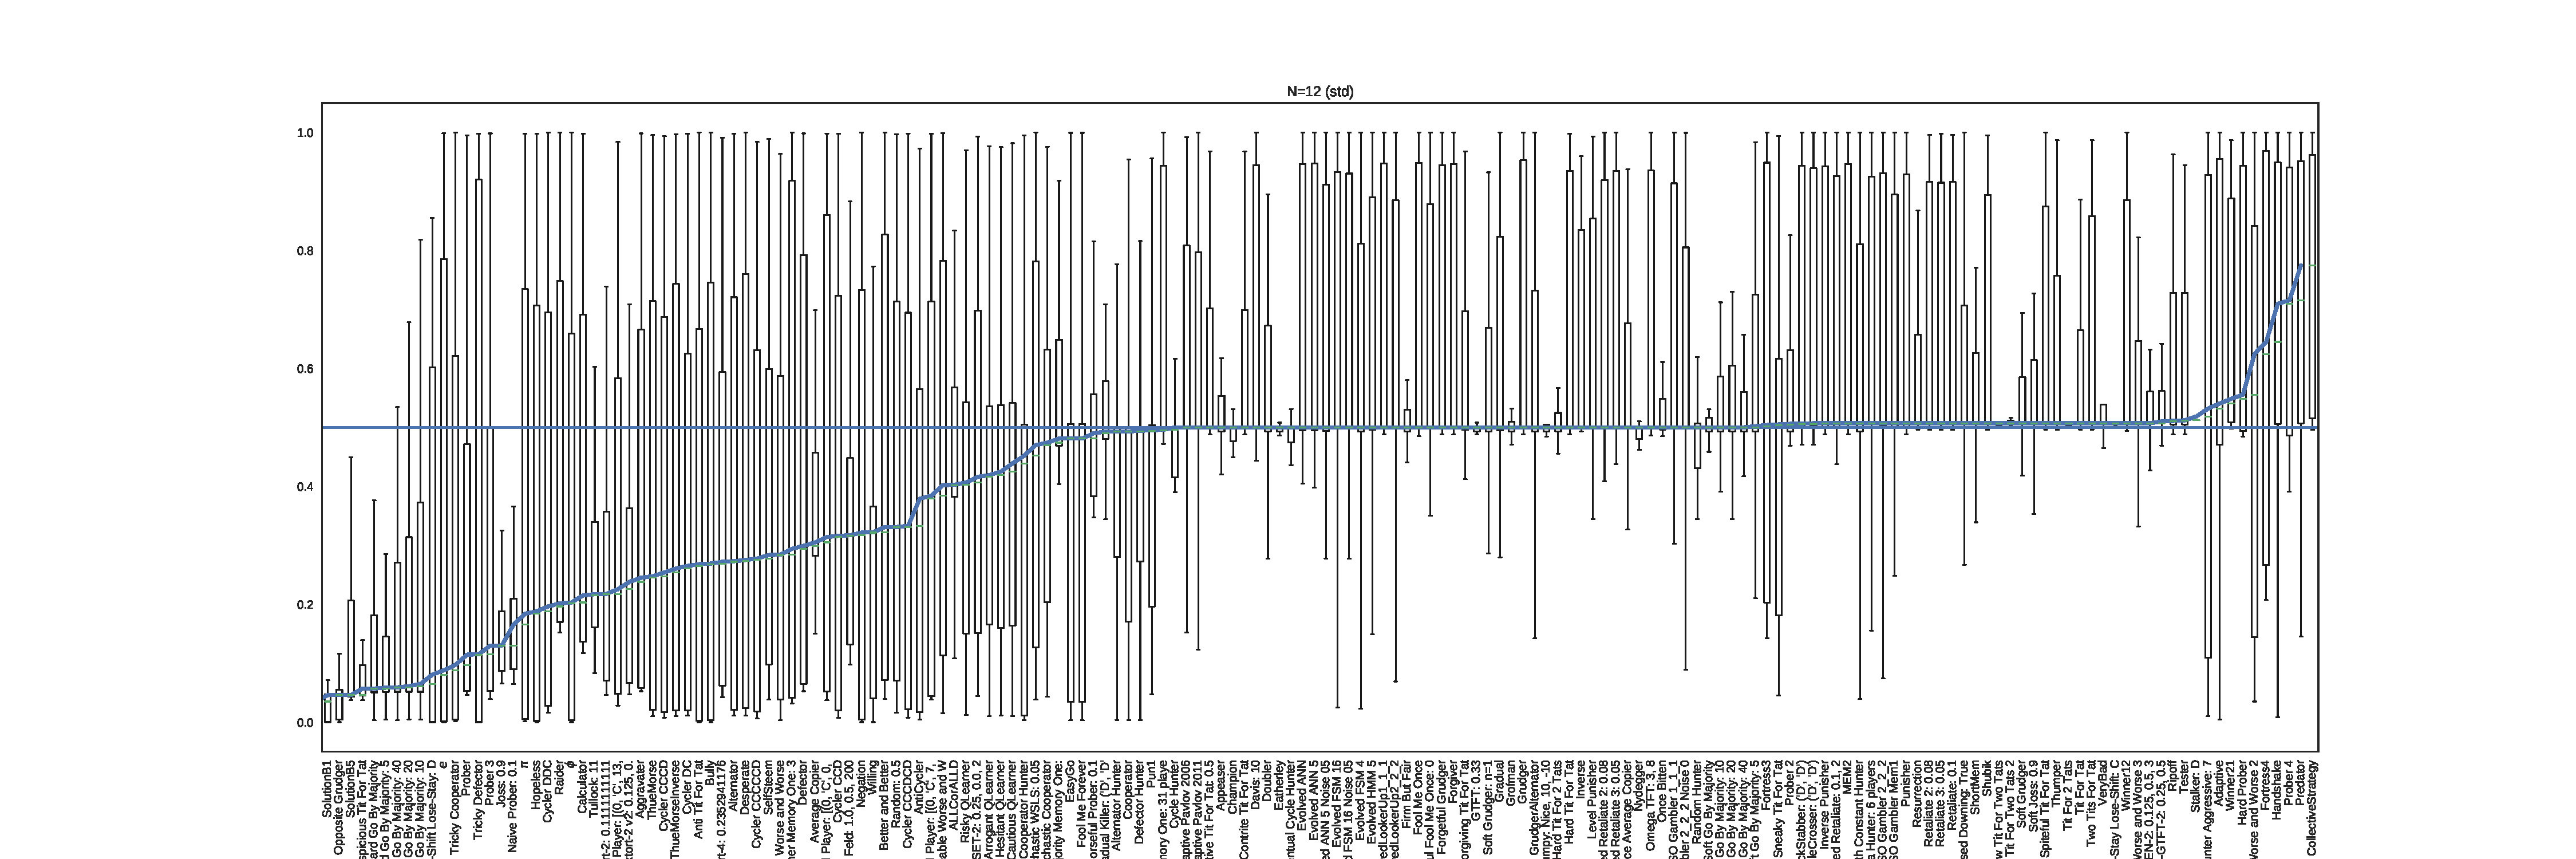
\includegraphics[width=\textwidth]{../img/fixation_boxplot_12_std.pdf}
        %\caption{\(N=12\)}
    %\end{subfigure}%

    \begin{subfigure}[t]{\textwidth}
        \centering
        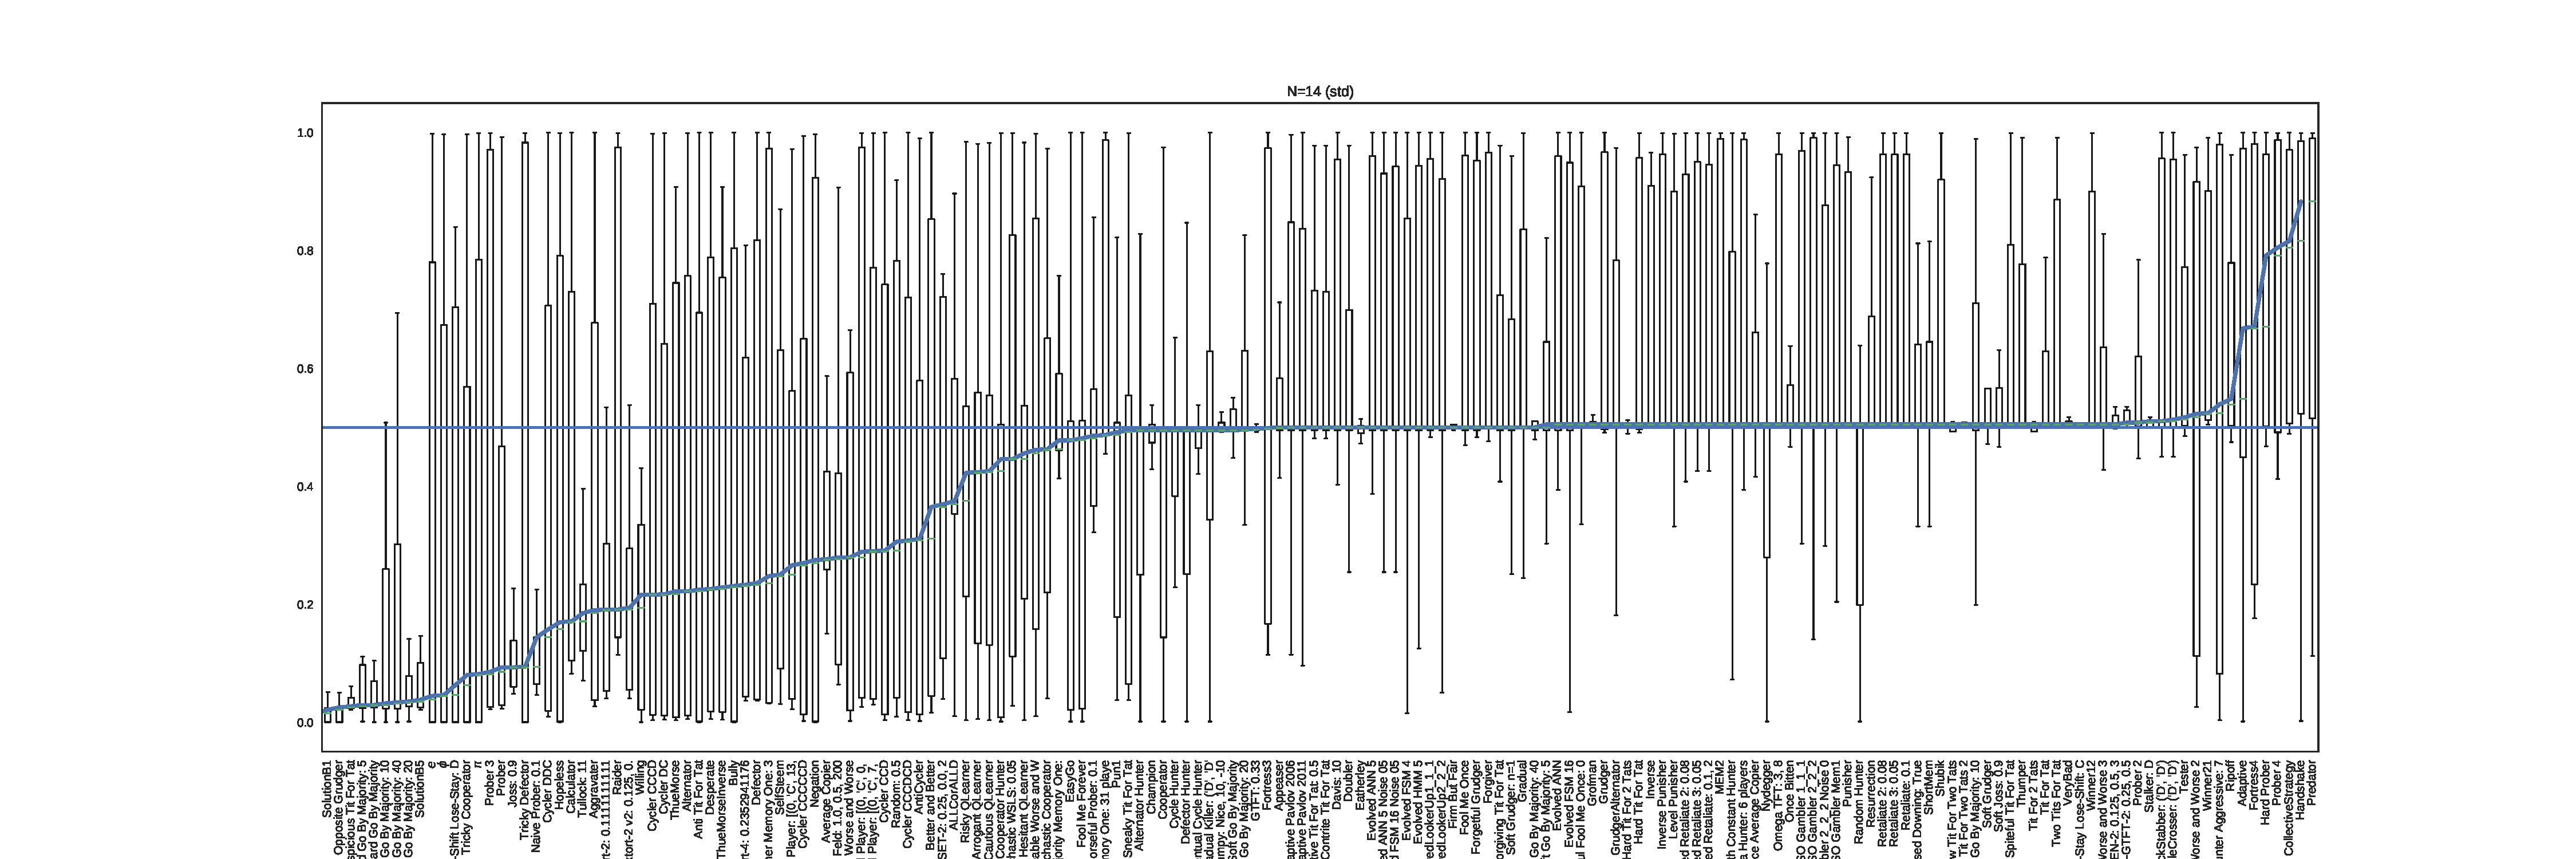
\includegraphics[width=\textwidth]{../img/fixation_boxplot_14_std.pdf}
        \caption{\(N=14\)}
    \end{subfigure}%
    \caption{Fixation probabilities of all strategies}
    \label{fig:fixation_boxplot_std}
\end{figure}

\begin{figure}[!hbtp]
    \centering
    \begin{subfigure}[t]{\textwidth}
        \centering
        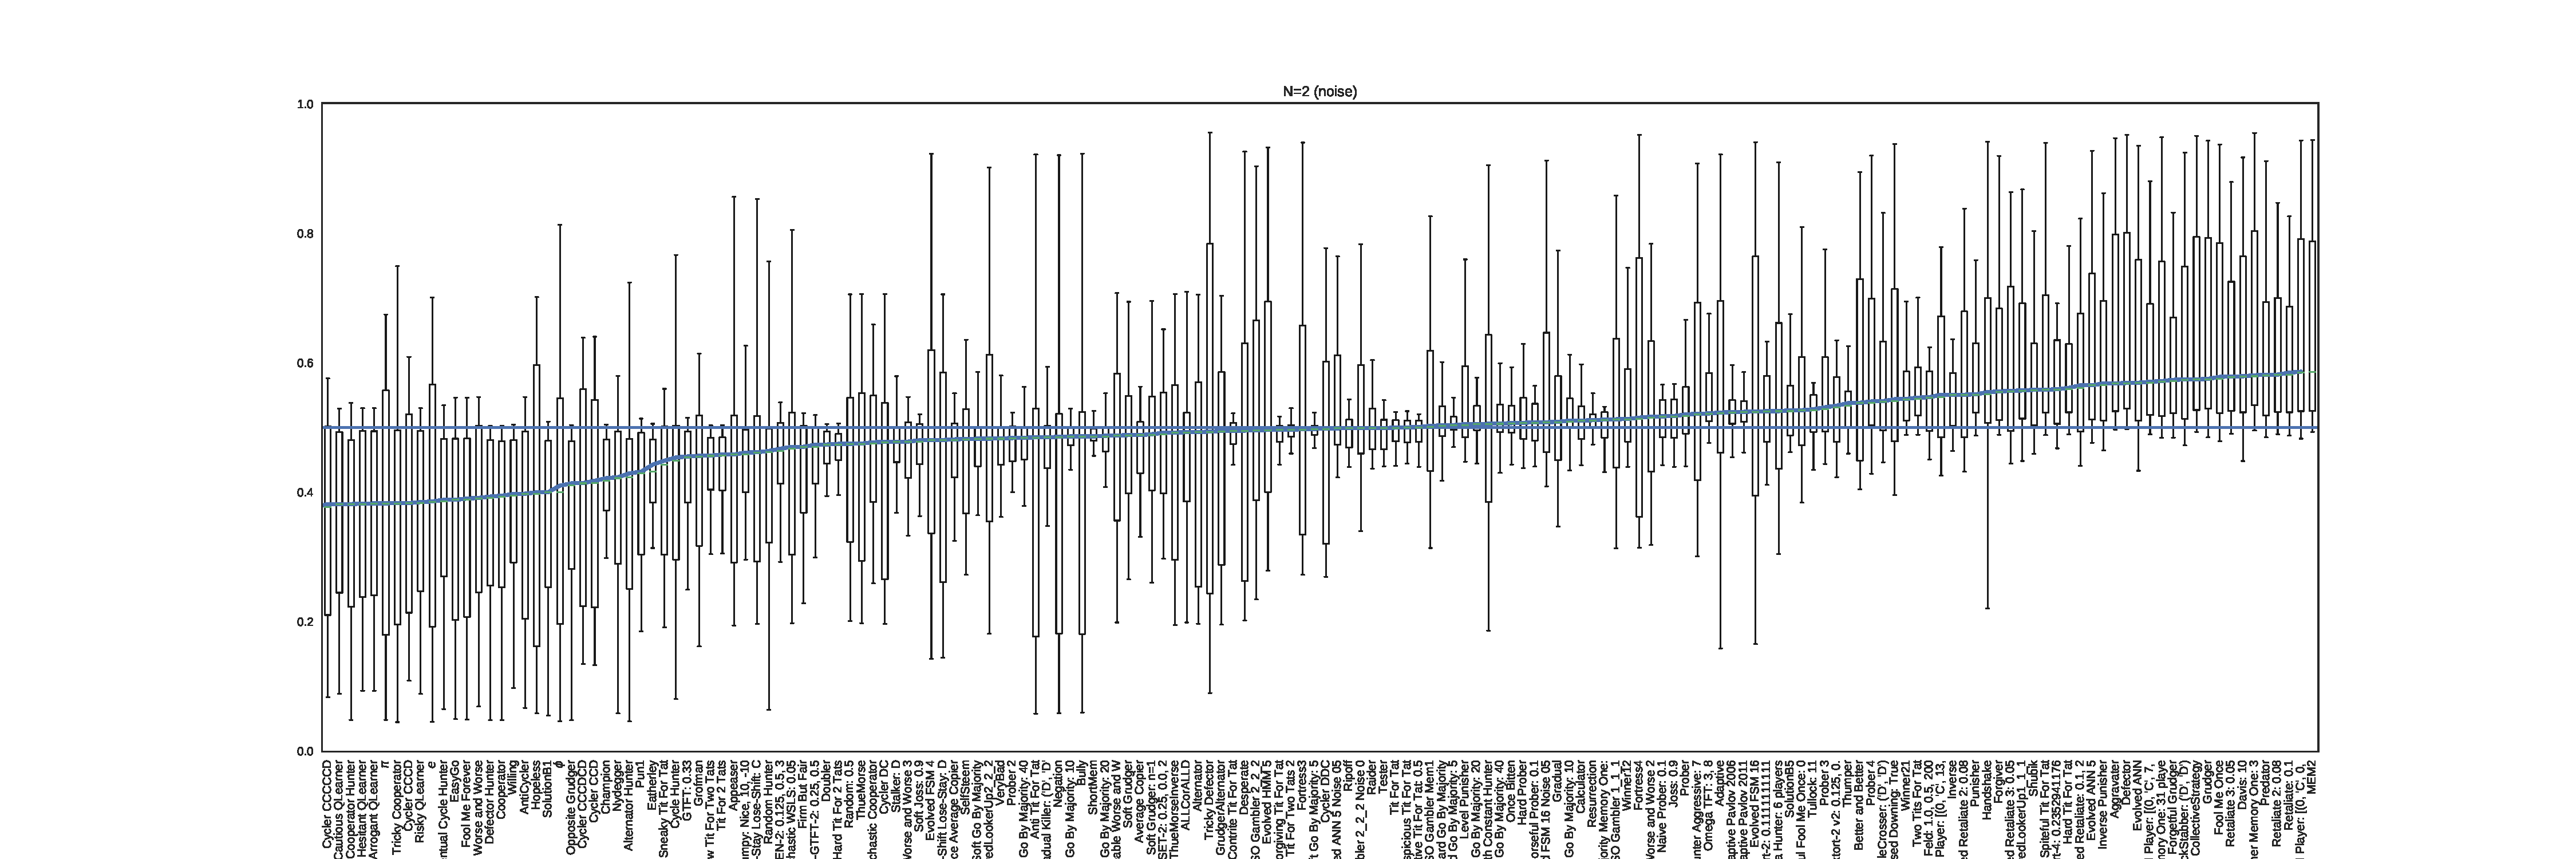
\includegraphics[width=\textwidth]{../img/fixation_boxplot_2_noise.pdf}
        \caption{\(N=2\)}
    \end{subfigure}%

    %\begin{subfigure}[t]{\textwidth}
        %\centering
        %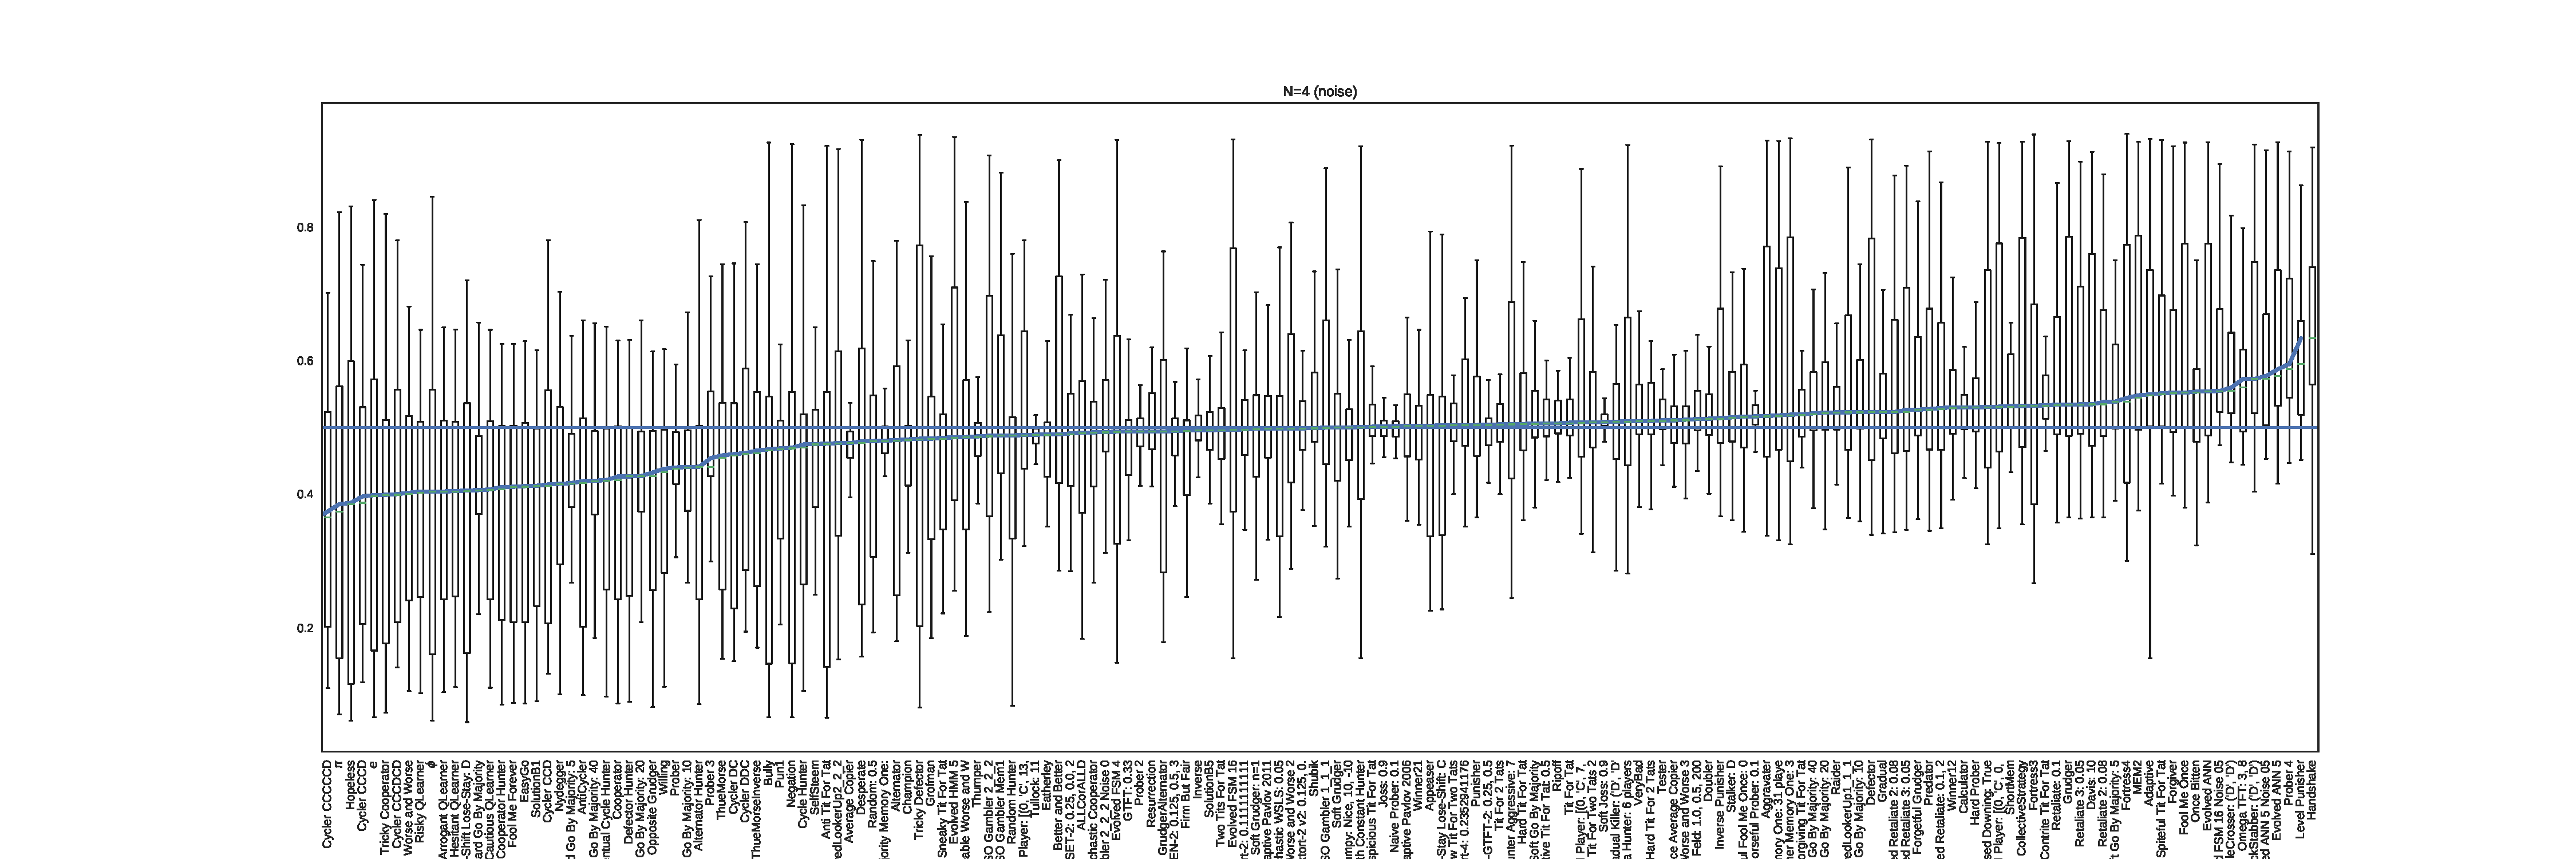
\includegraphics[width=\textwidth]{../img/fixation_boxplot_4_noise.pdf}
        %\caption{\(N=4\)}
    %\end{subfigure}%

    %\begin{subfigure}[t]{\textwidth}
        %\centering
        %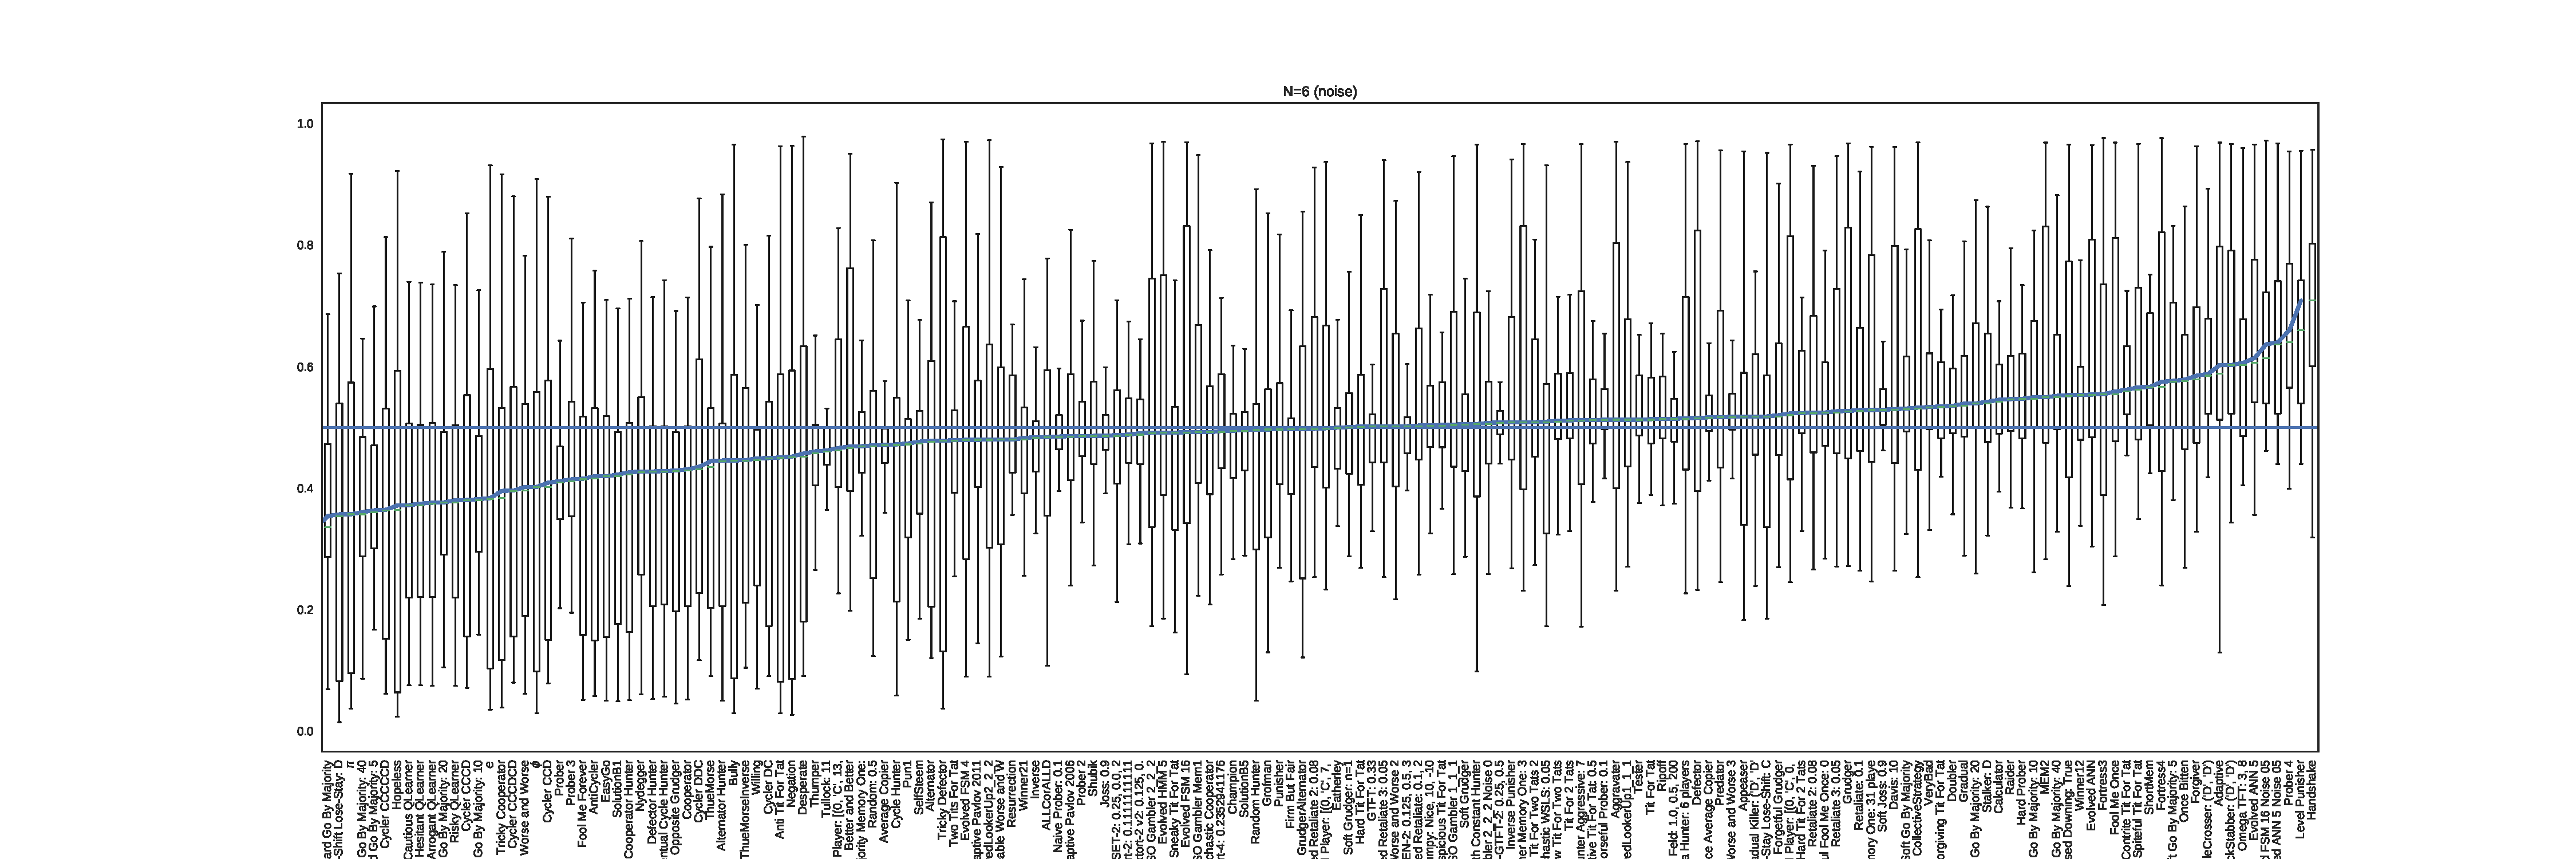
\includegraphics[width=\textwidth]{../img/fixation_boxplot_6_noise.pdf}
        %\caption{\(N=6\)}
    %\end{subfigure}%

    \begin{subfigure}[t]{\textwidth}
        \centering
        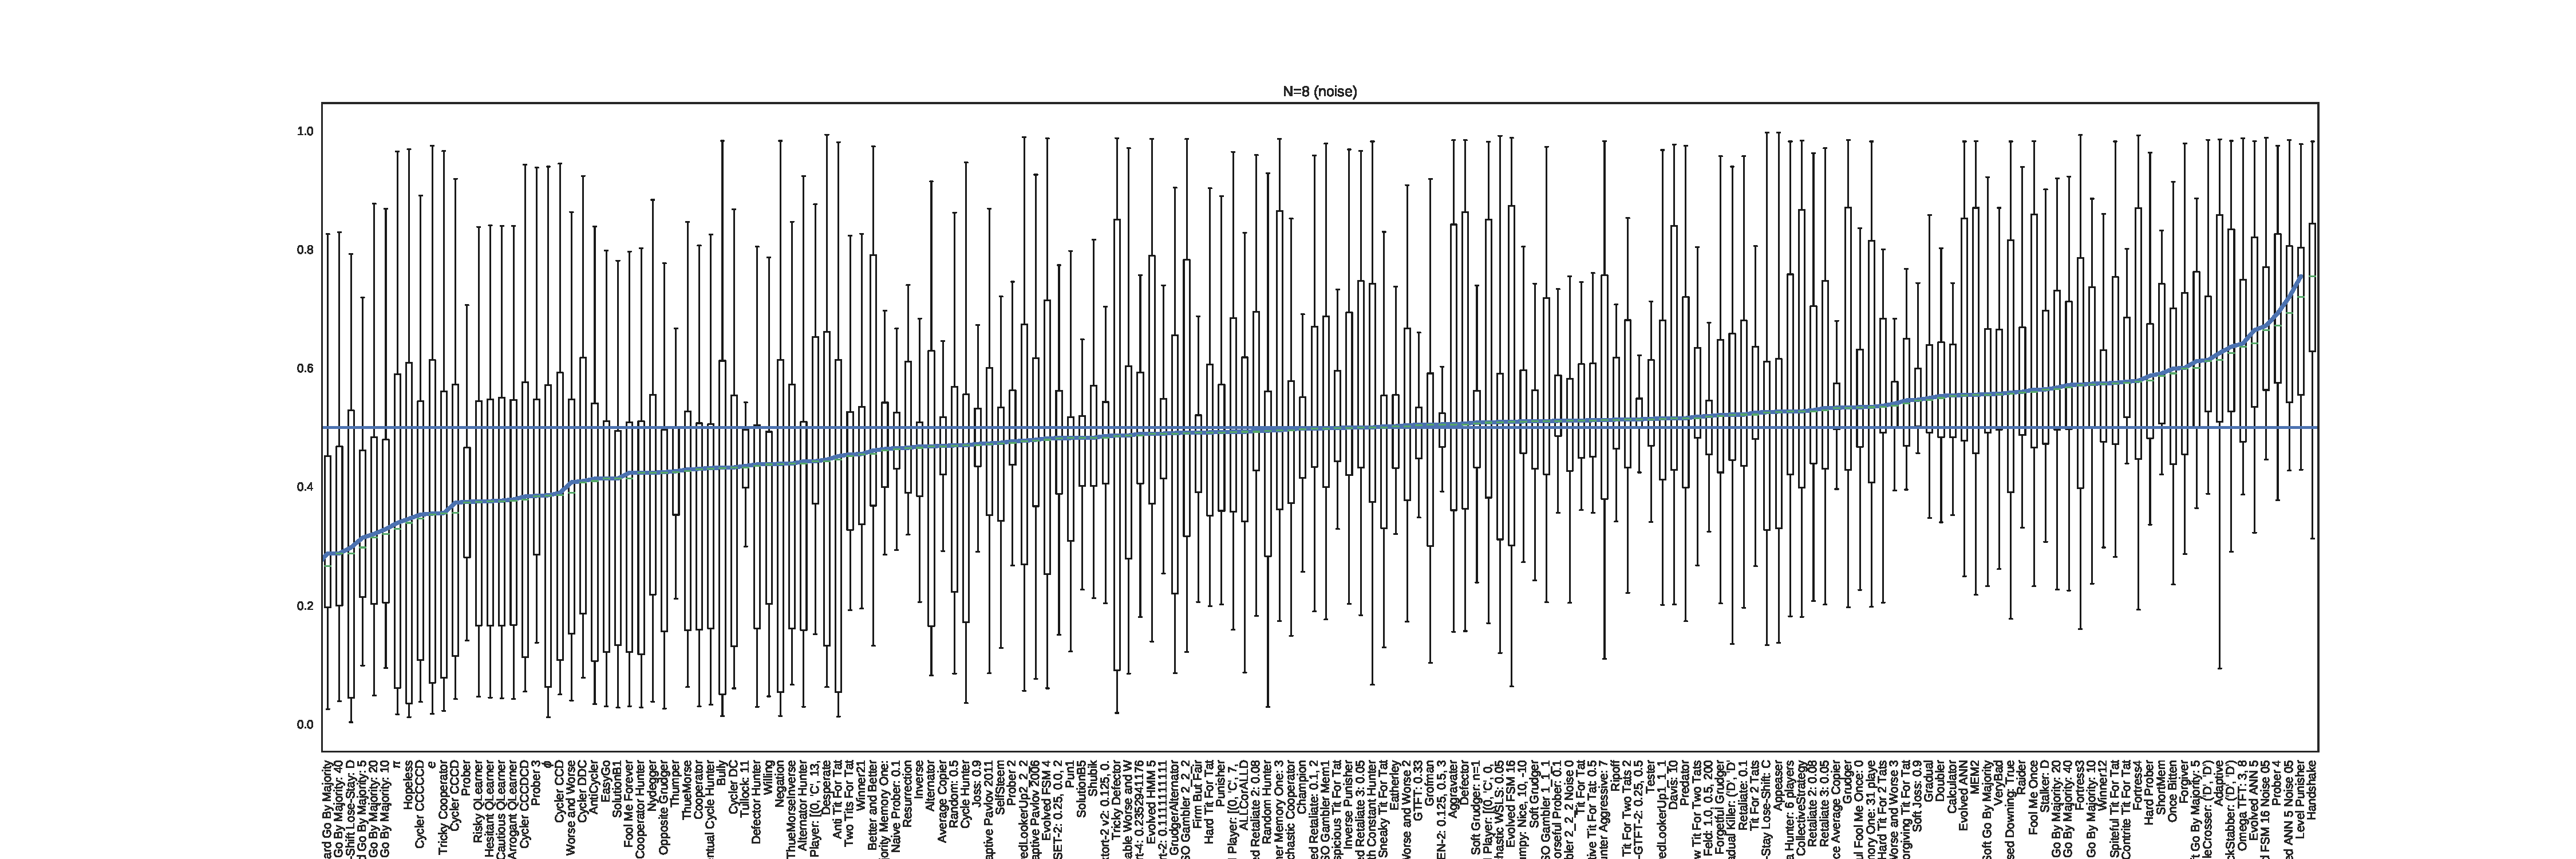
\includegraphics[width=\textwidth]{../img/fixation_boxplot_8_noise.pdf}
        \caption{\(N=8\)}
    \end{subfigure}%

    %\begin{subfigure}[t]{\textwidth}
        %\centering
        %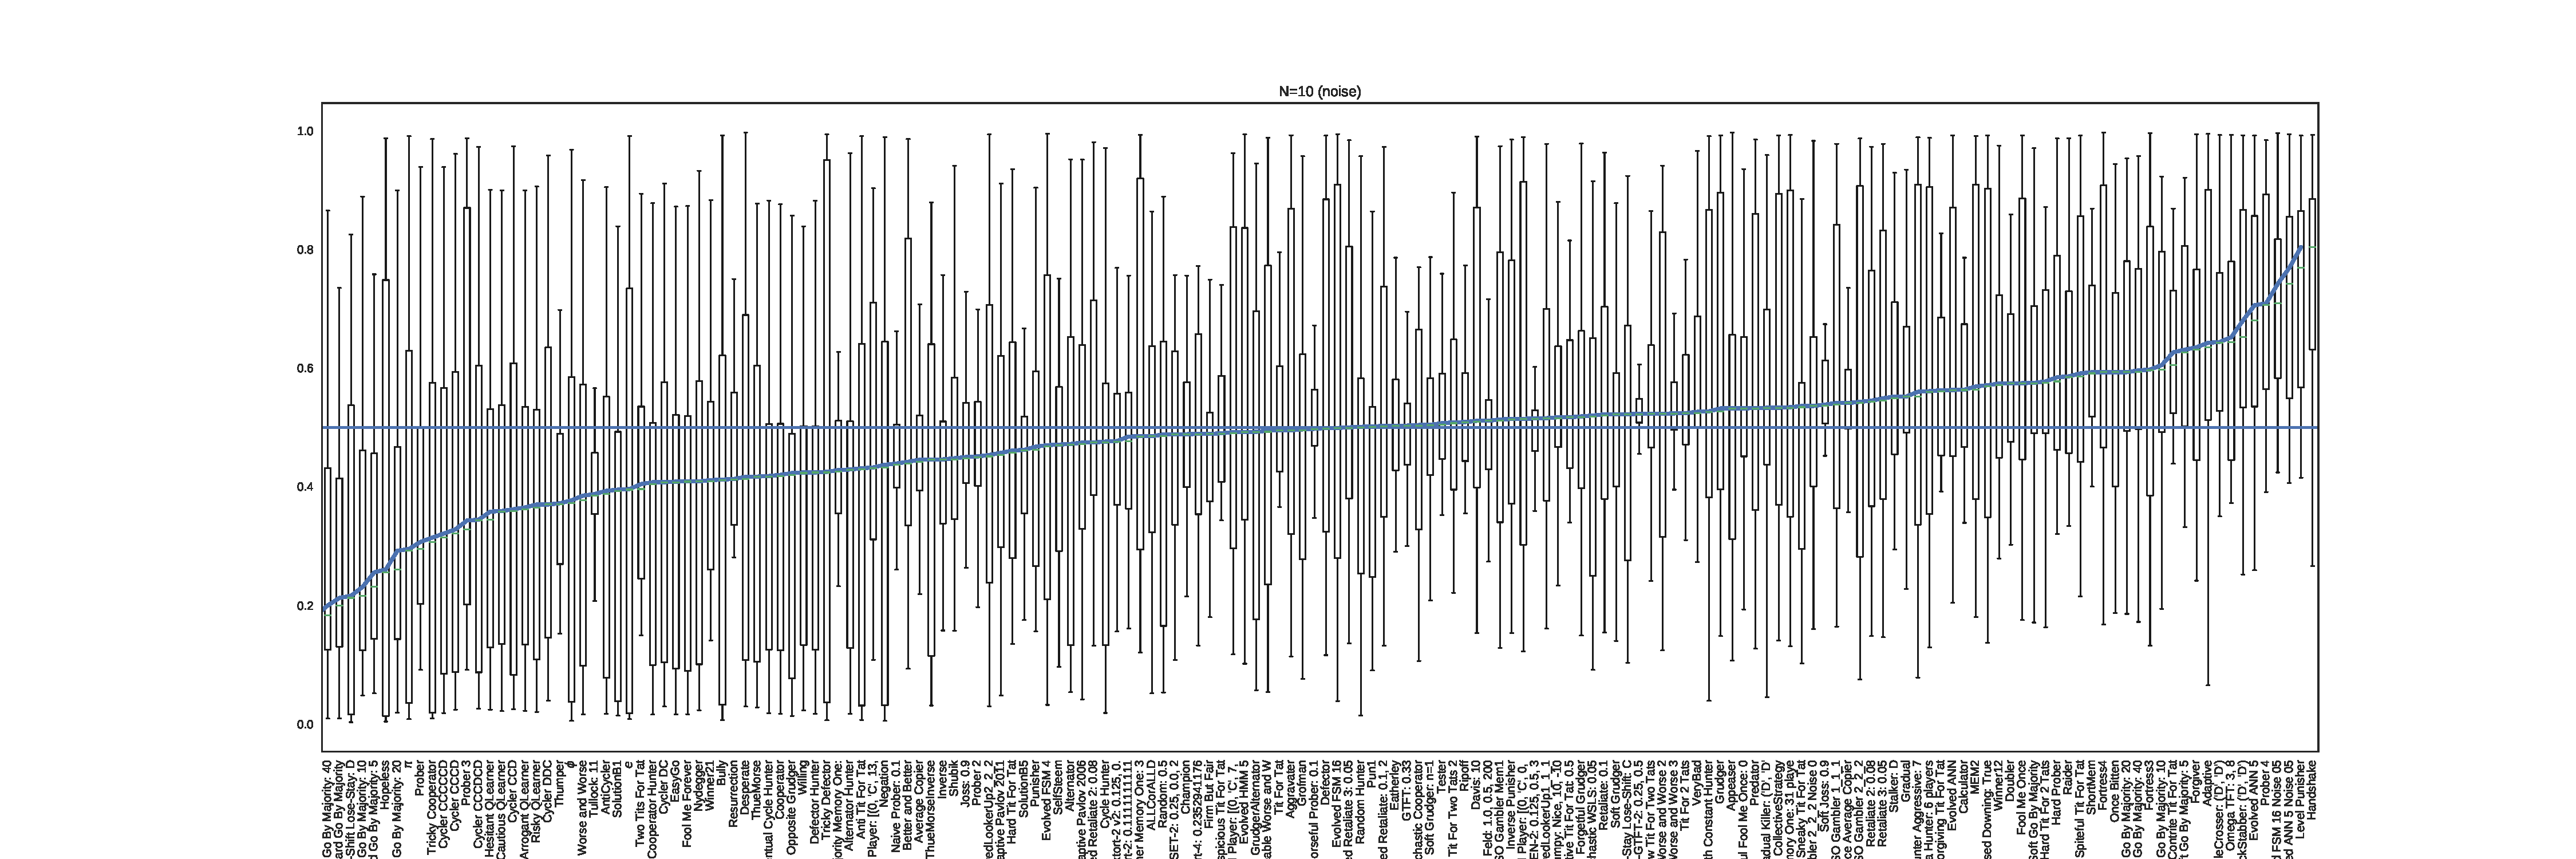
\includegraphics[width=\textwidth]{../img/fixation_boxplot_10_noise.pdf}
        %\caption{\(N=10\)}
    %\end{subfigure}%

    %\begin{subfigure}[t]{\textwidth}
        %\centering
        %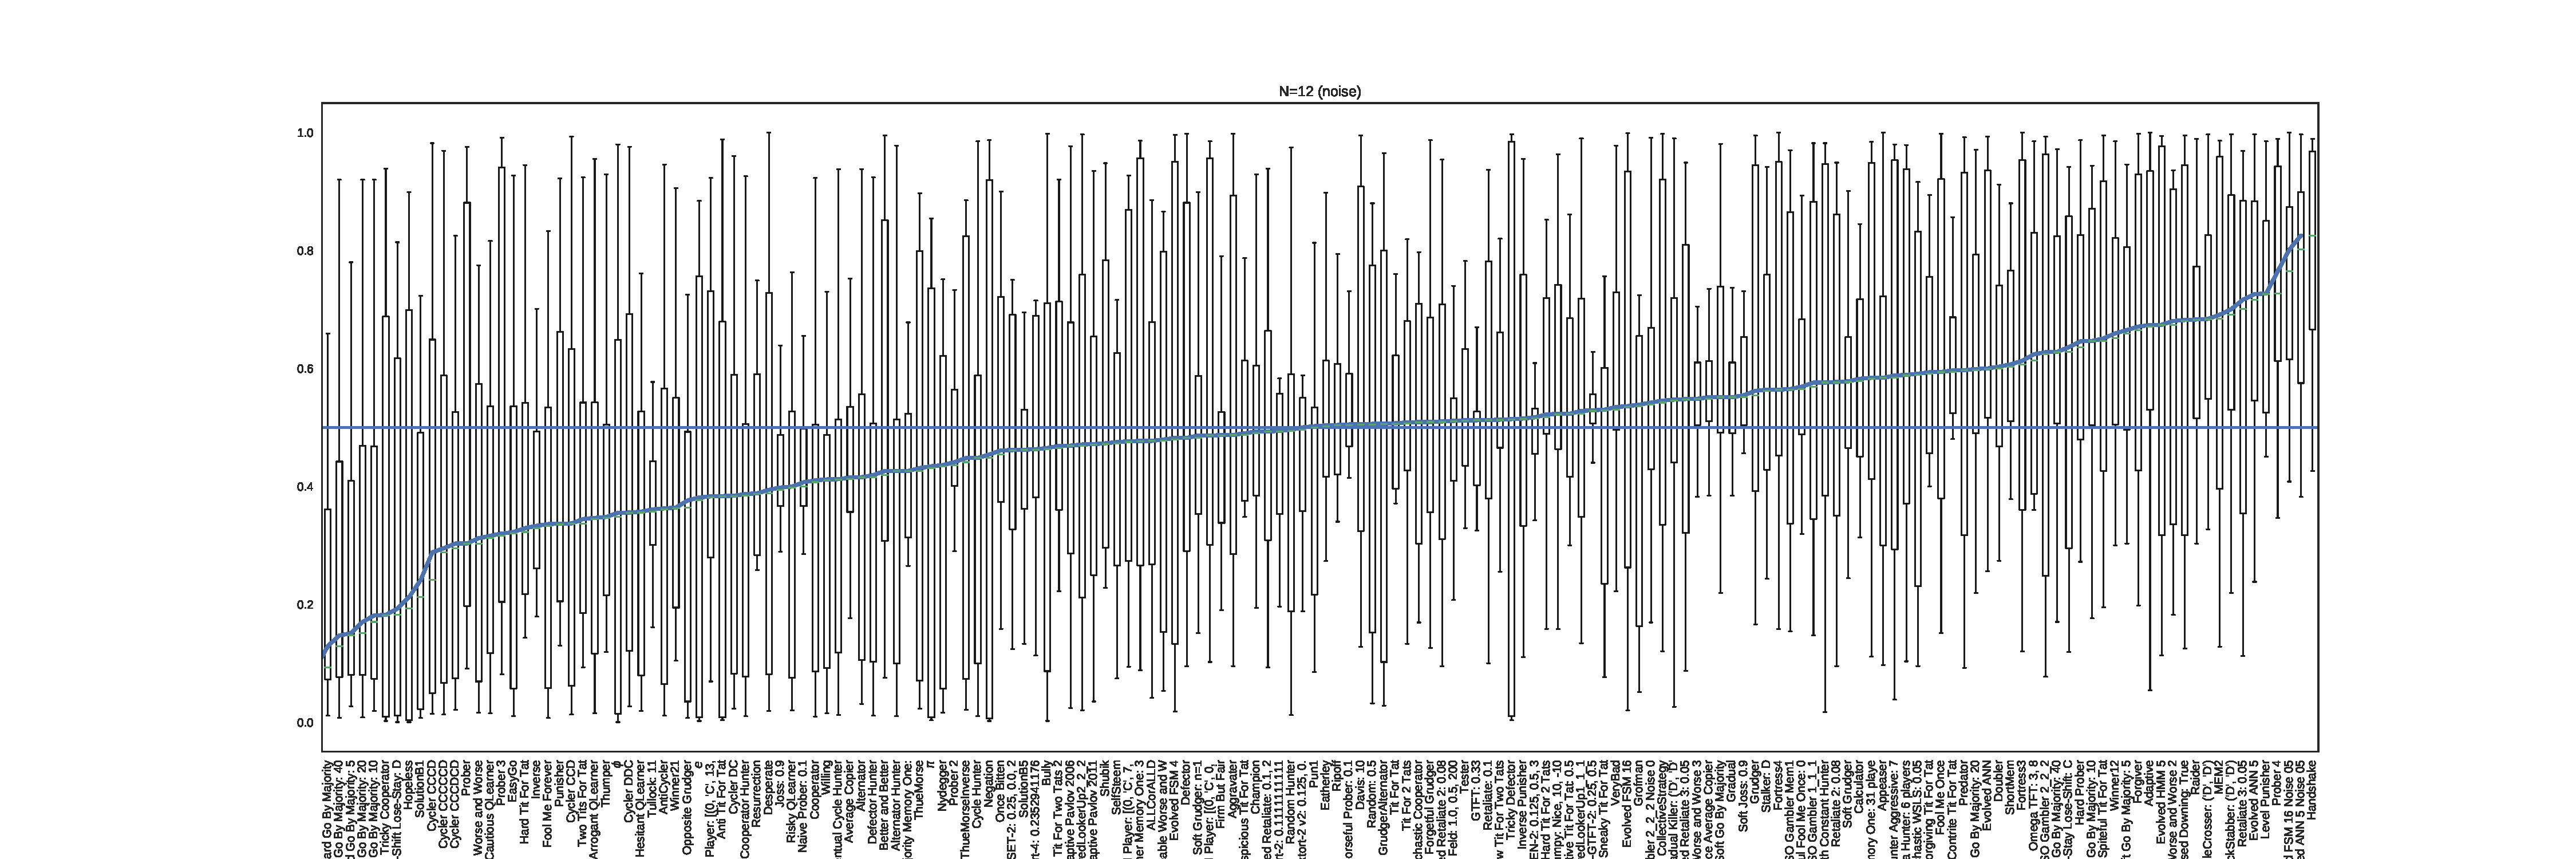
\includegraphics[width=\textwidth]{../img/fixation_boxplot_12_noise.pdf}
        %\caption{\(N=12\)}
    %\end{subfigure}%

    \begin{subfigure}[t]{\textwidth}
        \centering
        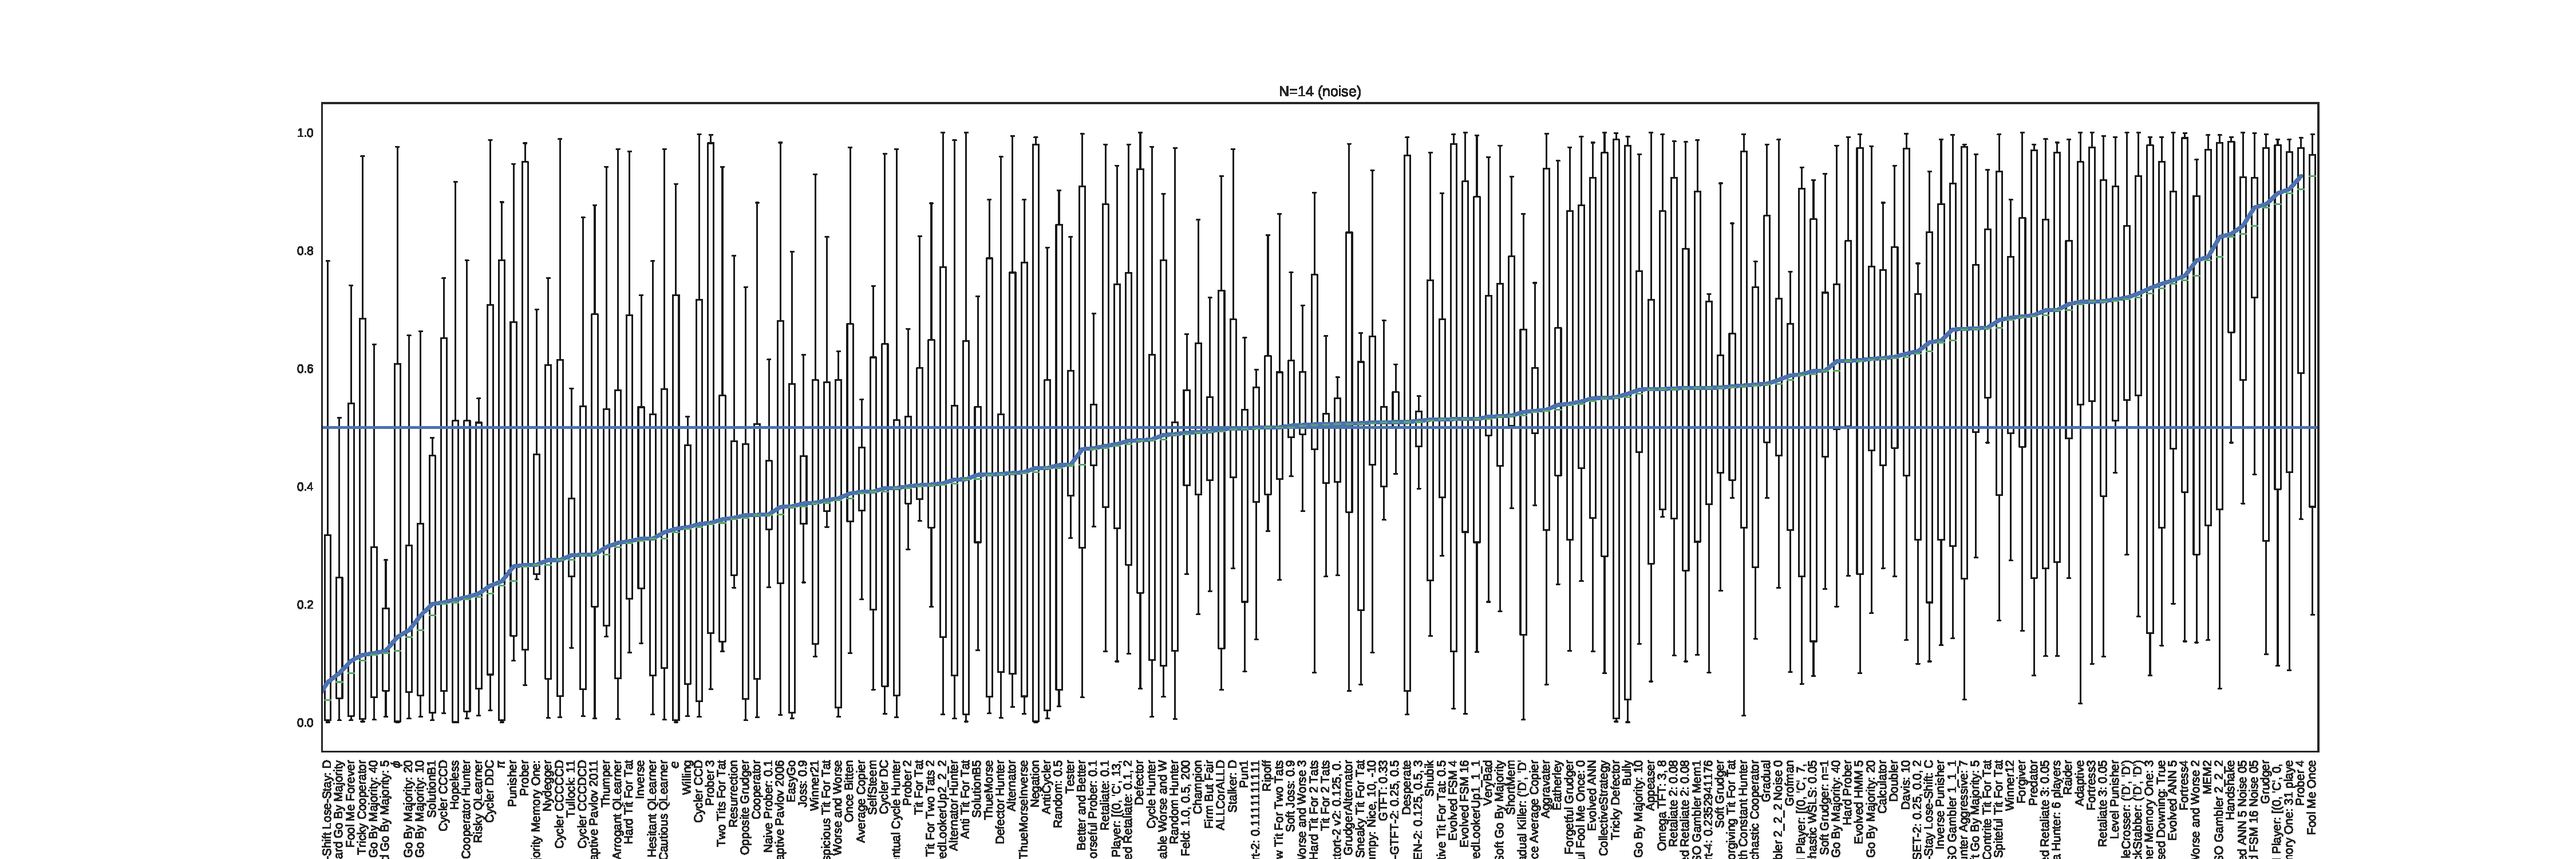
\includegraphics[width=\textwidth]{../img/fixation_boxplot_14_noise.pdf}
        \caption{\(N=14\)}
    \end{subfigure}%
    \caption{Fixation probabilities of all strategies (with noise)}
    \label{fig:fixation_boxplot_std}
\end{figure}

Figure~\ref{fig:histograms_median_fixation_rates_std}
and~\ref{fig:histograms_median_fixation_rates_noise} show the distribution of
the median fixation rates for all strategies.

\begin{figure}[!hbtp]
    \centering
    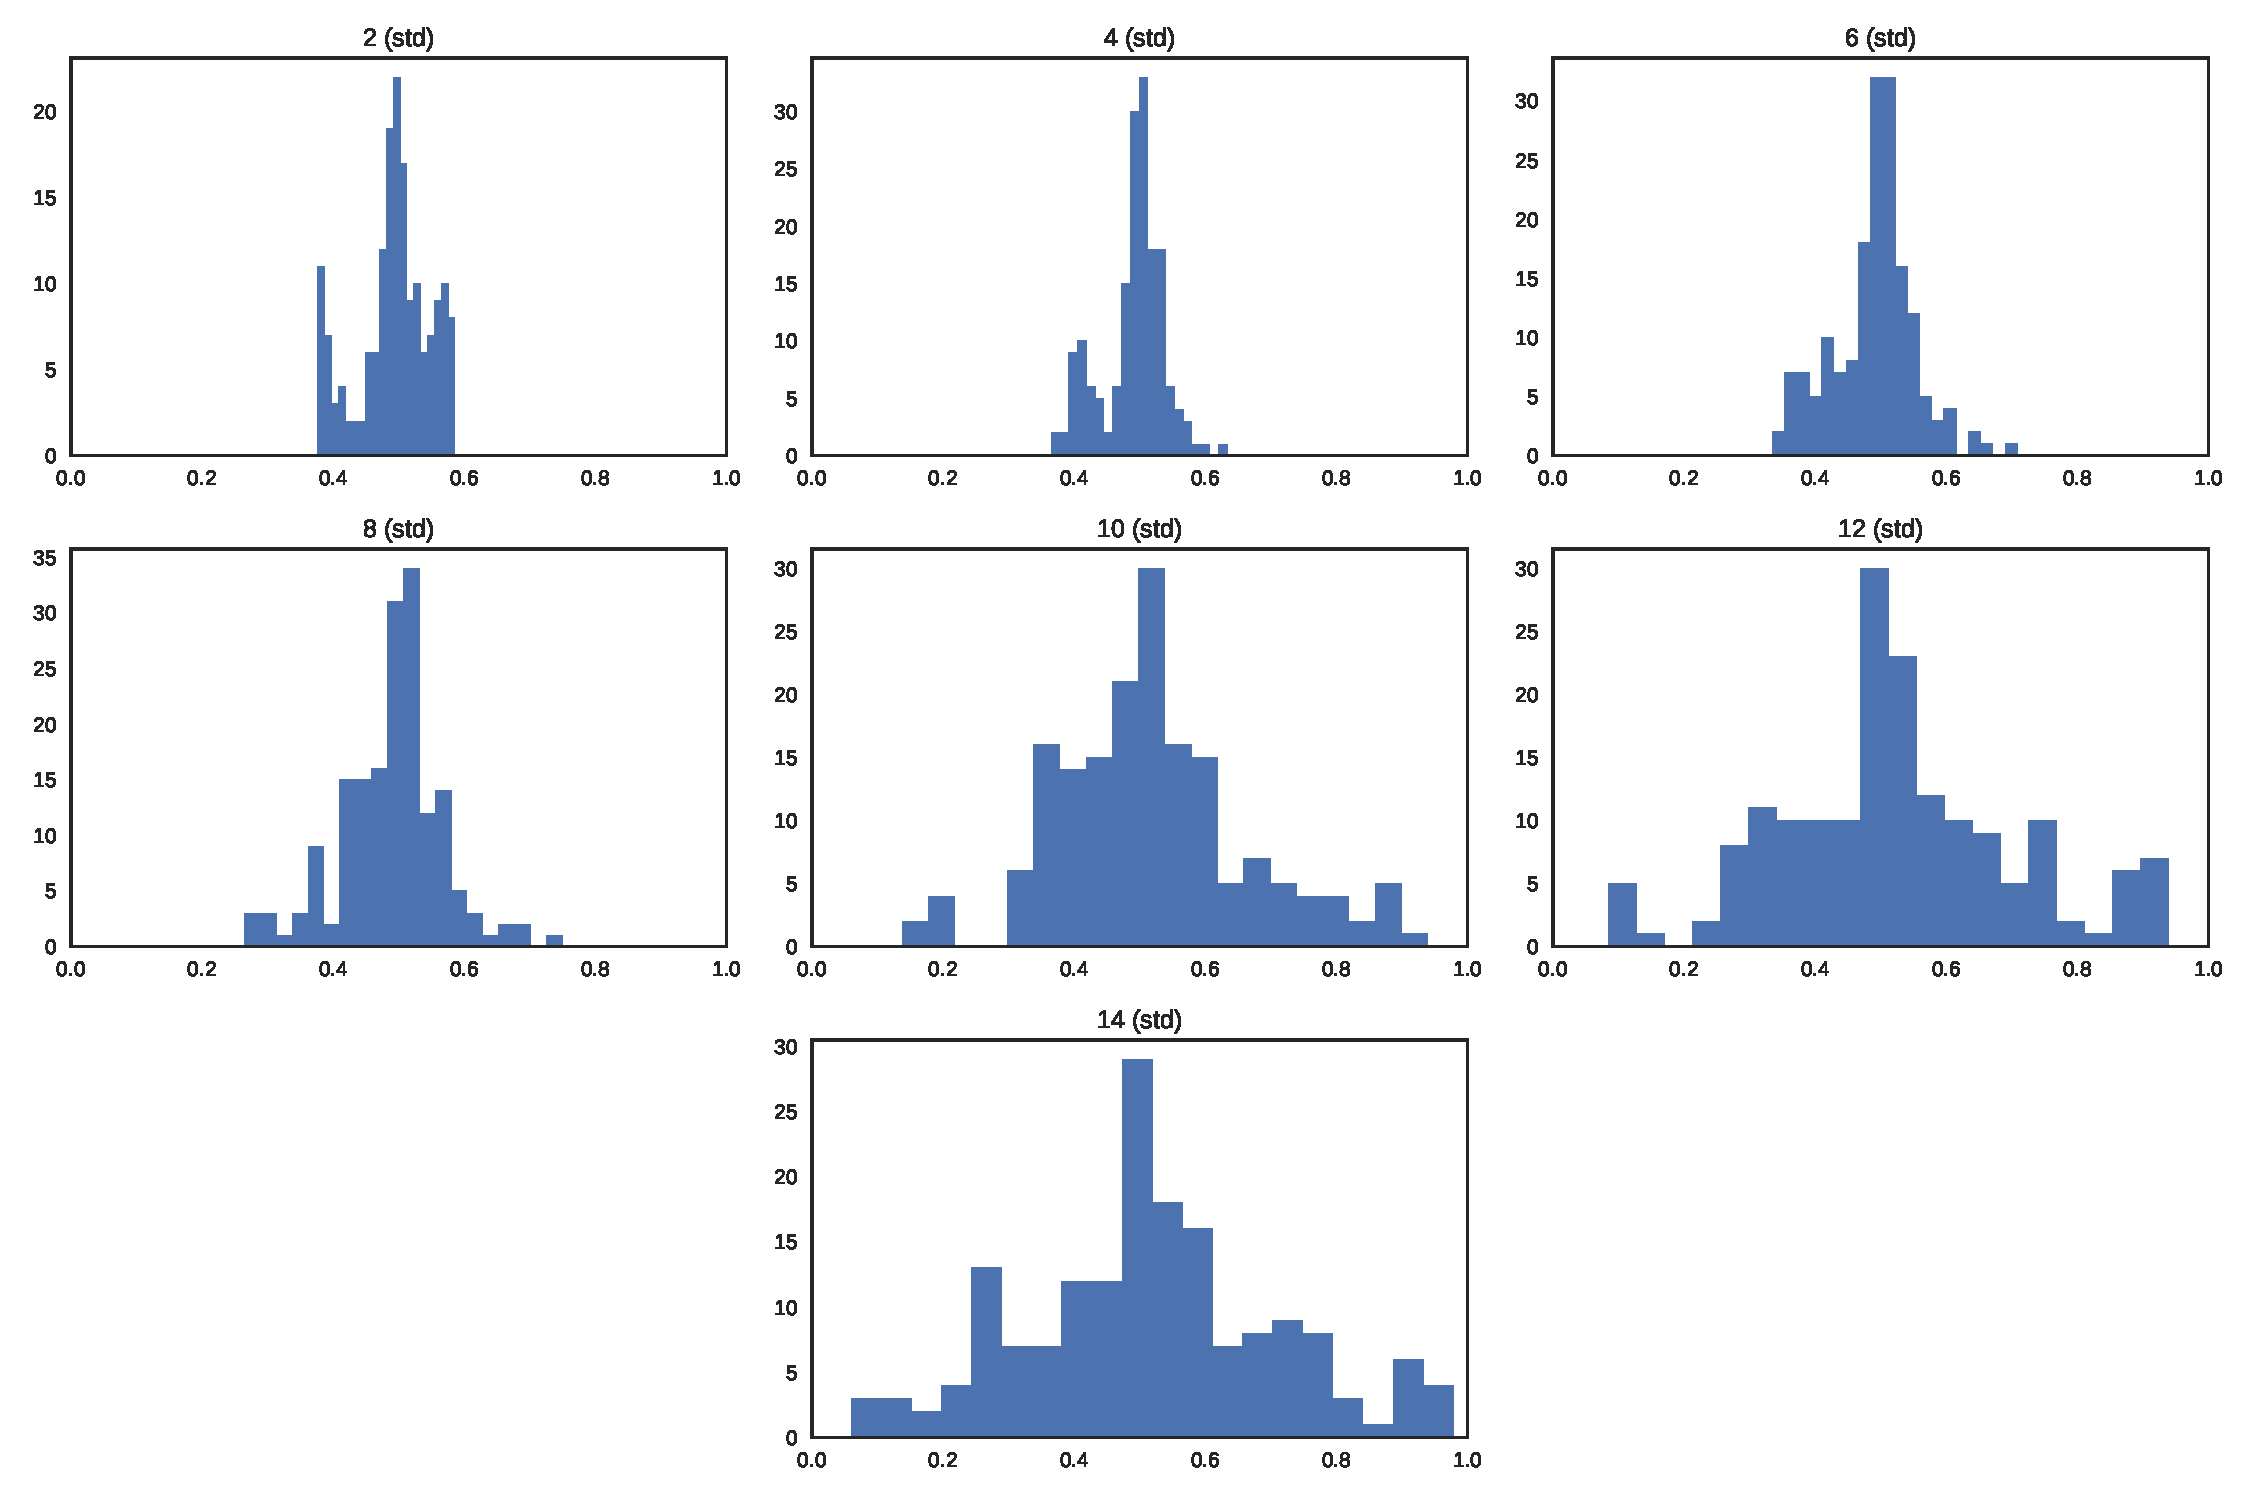
\includegraphics[width=.8\textwidth]{../img/histograms_median_fixation_rates_std.pdf}
    \caption{Distribution of median fixation rates for all players}
\end{figure}

\begin{figure}[!hbtp]
    \centering
    \includegraphics[width=.8\textwidth]{../img/histograms_median_fixation_rates_noise.pdf}
    \caption{Distribution of median fixation rates for all players (noise)}
\end{figure}

Figures~\ref{fig:ranks_v_size_standard} and~\ref{fig:ranks_v_size_noisy} show
the median rank of each strategy against population size in the standard and
noisy settings. Note that these ranks are not necessarily integers as group ties
are given the average rank.

\begin{figure}[!hbtp]

    \centering
    \begin{subfigure}{.5\textwidth}
    \centering
    \includegraphics[height=.9\textheight]{../img/median_rank_vs_population_size_std.pdf}
    \caption{Standard}
    \label{fig:ranks_v_size_standard}
    \end{subfigure}%
    ~
    \begin{subfigure}{.5\textwidth}
    \centering
    \includegraphics[height=.9\textheight]{../img/median_rank_vs_population_size_noisy.pdf}
    \caption{Noise}
    \label{fig:ranks_v_size_noisy}
    \end{subfigure}
    \caption{Median rank of players against population size}

\end{figure}

\begin{figure}[!hbtp]
    \centering
    \includegraphics[width=\textwidth]{../img/relationship_between_median_ranks_std.pdf}
    \caption{Relationship between Median rank for population size}
    \label{fig:relationship_ranks_v_size_standard}
\end{figure}

\begin{figure}[!hbtp]
    \centering
    \includegraphics[width=\textwidth]{../img/relationship_between_median_ranks_noisy.pdf}
    \caption{Relationship between Median rank for population size with noise}
    \label{fig:relationship_ranks_v_size_noise}
\end{figure}

Tables~\ref{tbl:ranks_in_size_2_std},~\ref{tbl:ranks_in_size_14_std},~\ref{tbl:ranks_in_size_2_noisy}
and~\ref{tbl:ranks_in_size_14_noisy} show the rankings across population size
based for the top on bottom performers across the extreme population sizes.

\begin{table}[!hbtp]
    \centering
        \begin{subfigure}[t]{\textwidth}
            \centering
                \begin{tabular}{lrrrrrrr}
\toprule
                                    Player &    2 &      4 &      6 &      8 &     10 &     12 &     14 \\
\midrule
 ZD-Extort-4: 0.23529411764705882, 0.25, 1 &  1.0 &  107.0 &  122.0 &  127.0 &  136.0 &  141.0 &  129.0 \\
        Meta Winner Memory One: 31 players &  2.0 &  113.5 &  120.5 &  126.0 &  126.0 &  133.0 &  132.0 \\
                       Feld: 1.0, 0.5, 200 &  3.0 &  106.0 &  116.0 &  121.0 &  123.0 &  127.0 &  128.0 \\
      ZD-Extort-2: 0.1111111111111111, 0.5 &  4.0 &  123.0 &  136.0 &  147.0 &  148.5 &  148.0 &  146.0 \\
             ZD-Extort-2 v2: 0.125, 0.5, 1 &  5.0 &  121.0 &  133.0 &  146.0 &  150.0 &  149.0 &  147.0 \\
\bottomrule
\end{tabular}

            \label{tbl:top_five_in_size_2_std}
        \end{subfigure}

        \begin{subfigure}[t]{\textwidth}
            \centering
                \begin{tabular}{lrrrrrrr}
\toprule
            Player &      2 &      4 &      6 &      8 &     10 &     12 &     14 \\
\midrule
     Cycler CCCCCD &  168.0 &  153.0 &  149.0 &  144.0 &  140.5 &  145.0 &  142.0 \\
               $e$ &  169.0 &  171.0 &  158.0 &  156.0 &  155.0 &  157.0 &  135.0 \\
       Cycler CCCD &  170.0 &  157.0 &  150.0 &  149.0 &  148.0 &  150.0 &  151.5 \\
 Tricky Cooperator &  171.0 &  158.5 &  152.0 &  150.0 &  136.0 &  159.0 &  101.0 \\
             $\pi$ &  172.0 &  172.0 &  159.0 &  159.0 &  156.0 &  147.5 &  131.0 \\
\bottomrule
\end{tabular}

            \label{tbl:bottom_five_in_size_2_std}
        \end{subfigure}%
        \caption{Performance across population sizes of top and bottom
        performing strategies in population size \(N=2\)}
        \label{tbl:ranks_in_size_2_std}
\end{table}


\begin{table}[!hbtp]
    \centering
        \begin{subfigure}[t]{\textwidth}
            \centering
                \begin{tabular}{lrrrrrrr}
\toprule
             Player &     2 &     4 &     6 &     8 &    10 &   12 &   14 \\
\midrule
          Fortress4 &  82.5 &  11.0 &   8.0 &   8.0 &   6.0 &  1.0 &  1.0 \\
          Fortress3 &  82.5 &  15.0 &  13.0 &  24.0 &  25.0 &  2.0 &  2.0 \\
           Predator &  11.0 &   2.0 &   2.0 &   2.0 &   1.0 &  3.0 &  3.0 \\
           Prober 4 &  15.0 &   3.0 &   3.0 &   3.0 &   2.0 &  4.0 &  4.0 \\
 CollectiveStrategy &   6.0 &   1.0 &   1.0 &   1.0 &   3.0 &  6.0 &  5.0 \\
\bottomrule
\end{tabular}

            \label{tbl:top_five_in_size_14_std}
        \end{subfigure}

        \begin{subfigure}[t]{\textwidth}
            \centering
                \begin{tabular}{lrrrrrrr}
\toprule
                  Player &      2 &      4 &      6 &      8 &     10 &     12 &     14 \\
\midrule
 Hard Go By Majority: 10 &   32.0 &  163.5 &  165.5 &  167.5 &  167.5 &  164.0 &  168.0 \\
  Hard Go By Majority: 5 &   32.0 &  163.5 &  165.5 &  167.5 &  167.5 &  167.5 &  169.0 \\
  Suspicious Tit For Tat &   38.0 &  163.5 &  165.5 &  167.5 &  167.5 &  170.0 &  170.0 \\
        Opposite Grudger &  140.0 &  167.0 &  171.0 &  171.0 &  171.0 &  170.0 &  171.0 \\
              SolutionB1 &  150.0 &  170.0 &  172.0 &  172.0 &  172.0 &  172.0 &  172.0 \\
\bottomrule
\end{tabular}

            \label{tbl:bottom_five_in_size_14_std}
        \end{subfigure}%
        \caption{Performance across population sizes of top and bottom
        performing strategies in population size \(N=14\)}
        \label{tbl:ranks_in_size_14_std}
\end{table}


\begin{table}[!hbtp]
    \centering
        \begin{subfigure}[t]{\textwidth}
            \centering
                \begin{tabular}{lrrrrrrr}
\toprule
                                            Player &    2 &     4 &     6 &     8 &    10 &     12 &     14 \\
\midrule
                                              MEM2 &  1.0 &  16.0 &  23.0 &   6.0 &   3.0 &   11.0 &    3.0 \\
 FSM Player: [(0, 'C', 0, 'C'), (0, 'D', 3, 'C'... &  2.0 &  28.0 &  46.0 &  26.5 &  18.0 &   13.0 &  137.0 \\
                                 Retaliate 2: 0.08 &  3.5 &  19.5 &  43.0 &  26.5 &  46.0 &   58.0 &   53.0 \\
                                    Retaliate: 0.1 &  3.5 &  23.0 &  40.0 &  58.0 &  87.5 &  112.0 &  108.0 \\
                                          Predator &  5.0 &  34.0 &  50.0 &  35.0 &  33.0 &   66.0 &    9.0 \\
\bottomrule
\end{tabular}

            \label{tbl:top_five_in_size_2_noisy}
        \end{subfigure}

        \begin{subfigure}[t]{\textwidth}
            \centering
                \begin{tabular}{lrrrrrrr}
\toprule
            Player &      2 &      4 &      6 &      8 &     10 &     12 &     14 \\
\midrule
 Arrogant QLearner &  168.0 &  162.0 &  163.0 &  158.0 &  152.0 &  145.0 &  155.5 \\
 Cautious QLearner &  170.0 &  158.0 &  165.0 &  156.0 &  153.0 &  138.0 &  138.0 \\
 Cooperator Hunter &  170.0 &  157.0 &  146.0 &  143.0 &  135.0 &  141.0 &  127.0 \\
 Hesitant QLearner &  170.0 &  162.0 &  164.0 &  159.0 &  134.0 &  129.0 &  121.0 \\
     Cycler CCCCCD &  172.0 &  172.0 &  167.0 &  165.0 &  166.0 &  157.5 &  152.0 \\
\bottomrule
\end{tabular}

            \label{tbl:bottom_five_in_size_2_noisy}
        \end{subfigure}%
        \caption{Performance across population sizes of top and bottom
        performing strategies in population size \(N=2\) (with noise)}
        \label{tbl:ranks_in_size_2_noisy}
\end{table}


\begin{table}[!hbtp]
    \centering
        \begin{subfigure}[t]{\textwidth}
            \centering
                \begin{tabular}{lrrrrrrr}
\toprule
            Player &      2 &      4 &      6 &      8 &     10 &     12 &   14 \\
\midrule
          Negation &  109.5 &  132.0 &  132.0 &  126.5 &  102.0 &  114.0 &  1.0 \\
          Prober 3 &   43.0 &  139.0 &  151.0 &  148.0 &   40.0 &  151.0 &  2.0 \\
              MEM2 &    1.0 &   16.0 &   23.0 &    6.0 &    3.0 &   11.0 &  3.0 \\
 PSO Gambler 2\_2\_2 &   92.0 &  115.0 &  100.5 &   17.0 &   12.0 &    3.0 &  4.0 \\
           Grudger &   10.5 &   21.5 &   37.0 &    8.0 &    2.0 &    2.0 &  5.0 \\
\bottomrule
\end{tabular}

            \label{tbl:top_five_in_size_14_noisy}
        \end{subfigure}

        \begin{subfigure}[t]{\textwidth}
            \centering
                \begin{tabular}{lrrrrrrr}
\toprule
                  Player &      2 &      4 &      6 &      8 &     10 &     12 &     14 \\
\midrule
 Hard Go By Majority: 40 &   71.0 &  149.0 &  169.5 &  170.5 &  172.0 &  171.0 &  168.0 \\
         Fool Me Forever &  160.5 &  156.0 &  150.0 &  146.0 &  141.0 &  151.0 &  169.0 \\
     Hard Go By Majority &   76.0 &  159.0 &  172.0 &  172.0 &  171.0 &  172.0 &  170.0 \\
       Tricky Cooperator &  166.5 &  167.0 &  157.0 &  162.0 &  166.0 &  166.0 &  171.0 \\
  Win-Shift Lose-Stay: D &  119.5 &  160.0 &  171.0 &  170.5 &  170.0 &  165.0 &  172.0 \\
\bottomrule
\end{tabular}

            \label{tbl:bottom_five_in_size_14_noisy}
        \end{subfigure}%
        \caption{Performance across population sizes of top and bottom
        performing strategies in population size \(N=14\) (with noise)}
        \label{tbl:ranks_in_size_14_noisy}
\end{table}

Table~\ref{tbl:median_rank_v_memory_length} shows the performance based on
memory length.

\begin{table}[!hbtp]
    \centering
        \begin{subfigure}[t]{\textwidth}
            \centering
                \begin{tabular}{rrrrrrrr}
\toprule
 Memory Depth &       2 &       4 &       6 &       8 &      10 &      12 &      14 \\
\midrule
            9 &   11.00 &    2.00 &    2.00 &    2.00 &    2.00 &    2.00 &    4.00 \\
            4 &   82.50 &   35.25 &   33.75 &   33.25 &   40.75 &   54.50 &   10.50 \\
           16 &   82.50 &   59.50 &   59.50 &   58.50 &   76.50 &   78.50 &   39.25 \\
           $\infty$ &   82.50 &   59.50 &   59.50 &   58.50 &   76.50 &   73.75 &   68.50 \\
            2 &   82.50 &   59.50 &   59.50 &   58.50 &   34.50 &   62.50 &   68.50 \\
            6 &   82.50 &   59.50 &   59.50 &   58.50 &   34.50 &   62.50 &   68.50 \\
           10 &   82.50 &   59.50 &   59.50 &   58.50 &   76.50 &   62.50 &   68.50 \\
           12 &   82.50 &   59.50 &   59.50 &   58.50 &   34.50 &   62.50 &   68.50 \\
            3 &   82.50 &   59.50 &   59.50 &   58.50 &   76.50 &   78.50 &   88.50 \\
            0 &  131.50 &  103.00 &  118.00 &  125.00 &  122.00 &  131.50 &  108.50 \\
           20 &   57.25 &  111.50 &  112.50 &  113.00 &  120.75 &  115.00 &  117.75 \\
           40 &   57.25 &  111.50 &  112.50 &  113.00 &  121.75 &  115.00 &  117.75 \\
            1 &   82.50 &  119.00 &  120.50 &  123.00 &  124.50 &  117.00 &  130.00 \\
          200 &    3.00 &  106.00 &  116.00 &  122.00 &  126.00 &  127.00 &  132.00 \\
            5 &   82.50 &  151.50 &  140.50 &  136.00 &  135.25 &  140.00 &  140.00 \\
           11 &   10.00 &  130.00 &  137.00 &  145.00 &  150.00 &  153.00 &  156.00 \\
\bottomrule
\end{tabular}

            \caption{Standard}
            \label{tbl:top_five_in_size_14_noisy}
        \end{subfigure}

        \begin{subfigure}[t]{\textwidth}
            \centering
                \begin{tabular}{rrrrrrrr}
\toprule
 Memory Depth &       2 &       4 &       6 &       8 &      10 &      12 &      14 \\
\midrule
            9 &    5.00 &   34.00 &   50.00 &   35.00 &   33.00 &   66.00 &    9.00 \\
           16 &   57.75 &   51.25 &   51.50 &   39.25 &   16.25 &   29.00 &   33.25 \\
            6 &  103.00 &   85.00 &   73.50 &   52.00 &   52.00 &   63.00 &   52.00 \\
           $\infty$ &   77.00 &   77.50 &   77.00 &   67.50 &   67.75 &   72.50 &   73.75 \\
            3 &  110.75 &   63.00 &   63.00 &   90.00 &  128.00 &  113.50 &   75.50 \\
            4 &   89.25 &   60.50 &   63.75 &   74.00 &   31.00 &   37.00 &   80.75 \\
            1 &  100.00 &  102.00 &  102.00 &  102.00 &  102.00 &   94.50 &   97.00 \\
          200 &   34.00 &   54.00 &   54.50 &   70.00 &   73.00 &   80.50 &  102.00 \\
           10 &  106.00 &   40.50 &   45.00 &   51.00 &   89.00 &   94.50 &  112.00 \\
           40 &   91.50 &   96.50 &   97.00 &  116.00 &  121.25 &  121.00 &  114.00 \\
            2 &   85.25 &   76.50 &   90.50 &  101.00 &  124.00 &  114.00 &  114.50 \\
            0 &  126.50 &  125.00 &  125.00 &  105.00 &   81.00 &   61.00 &  115.00 \\
           20 &   89.25 &   94.25 &   96.00 &  100.75 &  127.50 &  134.25 &  121.25 \\
           12 &   70.00 &   11.50 &   12.00 &   46.00 &  131.00 &  131.50 &  132.00 \\
            5 &   89.00 &  134.50 &  128.25 &  127.25 &  132.50 &  132.50 &  133.50 \\
           11 &   44.50 &  111.00 &  128.00 &  132.00 &  147.00 &  156.00 &  152.00 \\
\bottomrule
\end{tabular}

            \caption{Noisy}
            \label{tbl:bottom_five_in_size_14_noisy}
        \end{subfigure}%
        \caption{Median rank by memory length}
        \label{tbl:median_rank_v_memory_length}
\end{table}

% TODO Discuss effect of size on performance of strategies. Relate to Press and
% Dyson work: "ZD strategies win matches but not tournaments".
% TODO Include discussion about noise.

% TODO Redo everything with Meta strategies? This was a comment by MH. I suggest
% we leave this for this paper.

% TODO Discuss some particular interesting cases; strategies that perform well
% in the overall tournament for v2.8.0 perhaps?

\section{Conclusion}\label{sec:conclusion}

% TODO Write overall conclusion. (Perhaps: weakness of short memory
% strategies?)

Further work:

\begin{itemize}
    \item Spatial structure;
    \item More than two types in the population;
    \item Modified Moran processes (Fermi selection);
    \item Mutation;
\end{itemize}
% TODO Write this section.

\section*{Acknowledgements}

This work was performed using the computational facilities of the Advanced
Research Computing @ Cardiff (ARCCA) Division, Cardiff University.

\printbibliography

\appendix

\section{List of players}\label{app:list_of_players}

\begin{multicols}{3}
	\begin{enumerate}
		\item Hard Tit For Tat
\item Negation
\item Nice Average Copier
\item Nydegger
\item Winner21
\item Winner12
\item $\pi$
\item Win-Shift Lose-Stay: D
\item Omega TFT: 3, 8
\item Opposite Grudger
\item FSM Player: [(0, 'C', 13, 'D'), (0, 'D', 12, 'D'), (1, 'C', 3, 'D'), (1, 'D', 4, 'D'), (2, 'C', 14, 'D'), (2, 'D', 9, 'D'), (3, 'C', 0, 'C'), (3, 'D', 1, 'D'), (4, 'C', 1, 'D'), (4, 'D', 2, 'D'), (5, 'C', 12, 'C'), (5, 'D', 6, 'C'), (6, 'C', 1, 'C'), (6, 'D', 14, 'D'), (7, 'C', 12, 'D'), (7, 'D', 2, 'D'), (8, 'C', 7, 'D'), (8, 'D', 9, 'D'), (9, 'C', 8, 'D'), (9, 'D', 0, 'D'), (10, 'C', 2, 'C'), (10, 'D', 15, 'C'), (11, 'C', 7, 'D'), (11, 'D', 13, 'D'), (12, 'C', 3, 'C'), (12, 'D', 8, 'D'), (13, 'C', 7, 'C'), (13, 'D', 10, 'D'), (14, 'C', 10, 'D'), (14, 'D', 7, 'D'), (15, 'C', 15, 'C'), (15, 'D', 11, 'D')], 1, C
\item Once Bitten
\item Predator
\item FSM Player: [(0, 'C', 0, 'C'), (0, 'D', 3, 'C'), (1, 'C', 5, 'D'), (1, 'D', 0, 'C'), (2, 'C', 3, 'C'), (2, 'D', 2, 'D'), (3, 'C', 4, 'D'), (3, 'D', 6, 'D'), (4, 'C', 3, 'C'), (4, 'D', 1, 'D'), (5, 'C', 6, 'C'), (5, 'D', 3, 'D'), (6, 'C', 6, 'D'), (6, 'D', 6, 'D'), (7, 'C', 7, 'D'), (7, 'D', 5, 'C')], 1, C
\item Prober 2
\item Prober
\item Prober 3
\item Tricky Defector
\item Tullock: 11
\item VeryBad
\item Prober 4
\item Willing
\item Worse and Worse 2
\item Pun1
\item Two Tits For Tat
\item Tricky Cooperator
\item PSO Gambler 2\_2\_2
\item PSO Gambler 1\_1\_1
\item Tit For Tat
\item Worse and Worse
\item ZD-Extort-2: 0.1111111111111111, 0.5
\item Worse and Worse 3
\item Win-Stay Lose-Shift: C
\item Hard Tit For 2 Tats
\item Tit For 2 Tats
\item Hard Go By Majority
\item Cycle Hunter
\item Fool Me Once
\item ZD-GTFT-2: 0.25, 0.5
\item Adaptive
\item Cooperator Hunter
\item Forgiving Tit For Tat
\item Handshake
\item Eventual Cycle Hunter
\item Retaliate 3: 0.05
\item Forgetful Fool Me Once: 0.05
\item Adaptive Tit For Tat: 0.5
\item Forgiver
\item Revised Downing: True
\item Evolved ANN
\item Forgetful Grudger
\item Hard Go By Majority: 10
\item PSO Gambler 2\_2\_2 Noise 05
\item Cycler CCCCCD
\item Ripoff
\item Aggravater
\item Evolved ANN 5
\item Fortress3
\item Hard Go By Majority: 20
\item ZD-GEN-2: 0.125, 0.5, 3
\item ALLCorALLD
\item Hard Prober
\item Evolved ANN 5 Noise 05
\item SelfSteem
\item Alternator
\item Fortress4
\item Hard Go By Majority: 40
\item Cycler CCCD
\item Risky QLearner
\item FSM Player: [(0, 'C', 7, 'C'), (0, 'D', 1, 'C'), (1, 'C', 11, 'D'), (1, 'D', 11, 'D'), (2, 'C', 8, 'D'), (2, 'D', 8, 'C'), (3, 'C', 3, 'C'), (3, 'D', 12, 'D'), (4, 'C', 6, 'C'), (4, 'D', 3, 'C'), (5, 'C', 11, 'C'), (5, 'D', 8, 'D'), (6, 'C', 13, 'D'), (6, 'D', 14, 'C'), (7, 'C', 4, 'D'), (7, 'D', 2, 'D'), (8, 'C', 14, 'D'), (8, 'D', 8, 'D'), (9, 'C', 0, 'C'), (9, 'D', 10, 'D'), (10, 'C', 8, 'C'), (10, 'D', 15, 'C'), (11, 'C', 6, 'D'), (11, 'D', 5, 'D'), (12, 'C', 6, 'D'), (12, 'D', 9, 'D'), (13, 'C', 9, 'D'), (13, 'D', 8, 'D'), (14, 'C', 8, 'D'), (14, 'D', 13, 'D'), (15, 'C', 4, 'C'), (15, 'D', 5, 'C')], 1, C
\item Meta Hunter Aggressive: 7 players
\item Alternator Hunter
\item Evolved FSM 4
\item Cycler CCD
\item Slow Tit For Two Tats 2
\item $e$
\item Soft Go By Majority
\item Hard Go By Majority: 5
\item ShortMem
\item AntiCycler
\item Hesitant QLearner
\item Cycler DC
\item Evolved FSM 16
\item GTFT: 0.33
\item Slow Tit For Two Tats
\item Anti Tit For Tat
\item Shubik
\item General Soft Grudger: n=1,d=4,c=2
\item Soft Grudger
\item ZD-Extort-2 v2: 0.125, 0.5, 1
\item Soft Go By Majority: 10
\item Hopeless
\item Adaptive Pavlov 2006
\item Sneaky Tit For Tat
\item Inverse
\item Cycler DDC
\item Evolved FSM 16 Noise 05
\item Adaptive Pavlov 2011
\item Soft Go By Majority: 20
\item Inverse Punisher
\item PSO Gambler Mem1
\item SolutionB5
\item Appeaser
\item EvolvedLookerUp2\_2\_2
\item Joss: 0.9
\item Cycler CCCDCD
\item EvolvedLookerUp1\_1\_1
\item Punisher
\item Soft Go By Majority: 40
\item SolutionB1
\item Arrogant QLearner
\item Soft Go By Majority: 5
\item Defector
\item Level Punisher
\item Spiteful Tit For Tat
\item Raider
\item Soft Joss: 0.9
\item Meta Hunter: 6 players
\item Average Copier
\item Davis: 10
\item Limited Retaliate: 0.1, 20
\item Stochastic Cooperator
\item ZD-Extort-4: 0.23529411764705882, 0.25, 1
\item $\phi$
\item ZD-SET-2: 0.25, 0.0, 2
\item Better and Better
\item Limited Retaliate 2: 0.08, 15
\item Defector Hunter
\item Random Hunter
\item Stochastic WSLS: 0.05
\item Gradual
\item Limited Retaliate 3: 0.05, 20
\item Random: 0.5
\item Retaliate 2: 0.08
\item Remorseful Prober: 0.1
\item Suspicious Tit For Tat
\item Bully
\item Desperate
\item Gradual Killer: ('D', 'D', 'D', 'D', 'D', 'C', 'C')
\item Tester
\item CollectiveStrategy
\item Math Constant Hunter
\item Firm But Fair
\item Grofman
\item Feld: 1.0, 0.5, 200
\item ThueMorse
\item Cautious QLearner
\item Naive Prober: 0.1
\item Resurrection
\item Doubler
\item Fool Me Forever
\item Grudger
\item ThueMorseInverse
\item Evolved HMM 5
\item GrudgerAlternator
\item MEM2
\item Retaliate: 0.1
\item Contrite Tit For Tat
\item EasyGo
\item Calculator
\item Grumpy: Nice, 10, -10
\item Thumper
\item Cooperator
\item Eatherley

	\end{enumerate}
\end{multicols}

\end{document}
